% Neutral two-column preprint; no publisher template files are required.
\documentclass[10pt,a4paper,twocolumn]{article}
\usepackage[T1]{fontenc}
\usepackage[utf8]{inputenc}
\usepackage{amsmath,amssymb,amsthm}
\usepackage{stix2}
\renewcommand{\ttdefault}{lmtt}
\usepackage[a4paper,top=20mm,bottom=21mm,left=16mm,right=16mm,columnsep=6mm]{geometry}
\usepackage{graphicx,booktabs,array,multirow,tabularx,longtable}
\usepackage{etoolbox,placeins,pdflscape,dblfloatfix}
\usepackage{tikz,colortbl}
\usetikzlibrary{arrows.meta,positioning,shapes.geometric,calc,decorations.pathreplacing}
\usepackage[numbers,sort&compress]{natbib}
\usepackage{textcomp,xurl}
\usepackage[font=small,labelfont=bf,labelsep=period]{caption}
\usepackage{titlesec}
\usepackage{hyperref}
\hypersetup{colorlinks=true,linkcolor=black,citecolor=black,urlcolor=blue,
  pdftitle={Formalizing and Evaluating Rank Preservation in Empirical Monte Carlo Studies of Causal Estimators},
  pdfauthor={Carlos Ameal, Tom Loeys, Jan De Neve}}
\graphicspath{{figures/}}
\raggedbottom
\setlength{\parindent}{1em}
\setlength{\parskip}{0pt}
\setlength{\emergencystretch}{1em}
\titleformat{\section}{\large\bfseries}{\thesection}{0.65em}{}
\titleformat{\subsection}{\normalsize\bfseries}{\thesubsection}{0.65em}{}
\titleformat{\subsubsection}{\normalsize\itshape}{\thesubsubsection}{0.65em}{}
\titlespacing*{\section}{0pt}{2.2ex plus .5ex}{1ex}
\titlespacing*{\subsection}{0pt}{1.7ex plus .4ex}{.7ex}
\newlength{\tablegroupsep}
\setlength{\tablegroupsep}{8pt}
\newlength{\tablepanelgap}
\setlength{\tablepanelgap}{4pt}
\newcommand{\papertablestyle}{\fontsize{8}{10}\selectfont\setlength{\tabcolsep}{2pt}\renewcommand{\arraystretch}{1.05}}
\newcommand{\tablebox}[1]{\makebox[\linewidth][c]{#1}}
\AtBeginEnvironment{tabular}{\papertablestyle}
\AtBeginEnvironment{tabular*}{\papertablestyle}
\AtBeginEnvironment{longtable}{\papertablestyle\setlength{\LTcapwidth}{\linewidth}}
\newcommand{\supercite}[1]{\citep{#1}}
\newcommand{\authorcite}[1]{\citet{#1}}
\renewcommand{\figurename}{Figure}
\renewcommand{\tablename}{Table}
\begin{document}
\def\neutralpreprint{1}
\twocolumn[{
\begin{center}
{\LARGE\bfseries Formalizing and Evaluating Rank Preservation in Empirical Monte Carlo Studies of Causal Estimators\par}
\vspace{1em}
{\large Carlos Ameal\quad Tom Loeys\quad Jan De Neve\par}
\vspace{.5em}
{Ghent University\par}
\vspace{.3em}
{\small\href{mailto:carlos.rodriguezameal@ugent.be}{carlos.rodriguezameal@ugent.be}\par}
\end{center}
\vspace{.7em}
\begin{center}\textbf{Abstract}\end{center}
\begin{minipage}{\textwidth}
\small% !TeX root = Master.tex
Monte Carlo simulations are widely used to evaluate causal estimators and guide estimator selection in applied research. In empirical Monte Carlo studies, simulation models are often fitted to observed data and used to generate benchmark datasets with a specified target value for the causal estimand. However, it may be unclear whether the resulting benchmarks reproduce the conclusions that would have been obtained under the original data-generating process. In this paper, we formalize benchmarks in empirical Monte Carlo studies as pairs consisting of a dataset law and a reference estimand value, which are designed to approximate an unavailable target benchmark under the unknown data-generating process. To illustrate our framework and gain empirical evidence, we employ two established collections of data-generating designs from the causal-inference literature to compare outcome simulators in their ability to preserve estimator rankings and guide estimator selection. We focus particularly on bias arising from sharing model families with candidate estimators. We assess agreement between target and simulator-induced benchmarks using rank correlations. Results show that simulators often preserve rankings well, but with substantial variability across models and settings. Sharing model families with candidate estimators can distort their rankings, particularly when the simulation model struggles to capture the underlying outcome structure. In these cases, simulator-guided selection can improve on direct estimation after excluding aligned estimators, whereas direct estimation can be preferable when those models perform well. Finally, distances between observed and simulated outcome distributions were somewhat informative, particularly for ruling out very poorly performing simulators.
\par
\vspace{.6em}
\noindent\textbf{Keywords:} causal inference; empirical Monte Carlo studies; plasmode; simulation; estimator selection; benchmarking.
\end{minipage}
\vspace{1.6em}
}]
% !TeX root = Master.tex
\section{Introduction}
\label{sec:introduction}
It is common for a researcher working on an applied study to struggle with the choice of a statistical method. For prediction, models can be tested by setting aside part of the initial sample as a test set and comparing predictions against observed outcomes. However, much current scientific research, particularly in fields such as medicine and economics, seeks to answer causal questions, often requiring the estimation of counterfactuals, which are unobserved by definition. Therefore, causal estimates cannot be evaluated against an observed ground truth.

Theoretical properties can guide this choice, but asymptotic approximations may be inaccurate in small samples. Also, relationships between variables may be complex, and non-ideal scenarios such as limited overlap or confounding are common. To circumvent this issue, researchers have tested these estimators on constructed datasets in controlled scenarios with a specified reference value for the estimand. By comparing estimates to this value, they can obtain an estimation error per dataset, and by aggregating and averaging over datasets, they can compute metrics that allow researchers to rank the estimators according to their performance.

This general strategy is known as a \emph{Monte Carlo benchmark study}. The degree to which conclusions drawn from such studies can be useful in a particular real-world setting depends on how well the simulation mechanism reproduces the features of the target data-generating process (DGP) that determine estimator performance. To improve realism, empirical data are increasingly used to construct Monte Carlo datasets. In the econometrics literature, studies using this approach are referred to as \emph{empirical Monte Carlo studies} (EMCS). \authorcite{advaniMostlyHarmlessSimulations2019} distinguish \emph{placebo designs}, in which the treated sample is selected from an empirical control group using an artificial propensity score, so causal effects are known to be null, from \emph{structured designs}, in which the empirical DGP is modeled and data are generated from that model to approximate the original process. In medicine and epidemiology, the related trend has been associated with \emph{statistical plasmodes}, which can be seen as a subset of EMCS in which covariates are resampled from empirical data and outcomes are generated using an outcome-generating model \cite{schreckStatisticalPlasmodeSimulations2024}.

In this paper, we propose a framework that formalizes an EMCS benchmark as a pair consisting of two distinct objects. The first is a dataset-level distribution from which full simulated datasets are generated, intended to approximate the target redrawing scheme under the unknown distribution that generated the observed data. This law determines the ideal sampling behavior of the estimators. The second is a benchmark value for the estimand of interest, against which estimates are compared. In Section~\ref{sec:framework}, we make explicit the assumptions underlying this construction and define the conditions under which a constructed benchmark can be considered useful for estimator comparison.

Traditionally, studies benchmarked estimators (often newly proposed ones) under user-specified DGPs. These DGPs have been criticized as simplistic or unrealistic~\supercite{huberPerformanceEstimatorsBased2013,gentzelCaseEvaluatingCausal,boulesteixIntroductionStatisticalSimulations2020}. In this study, we focus on structured EMCS, which aim to approximate the DGP behind a reference dataset, providing context-specific information about estimator performance that may help reduce model uncertainty. From now on, EMCS refers to structured EMCS. In response to these criticisms, flexible generative models have gained attention. For example, to avoid researcher-specified DGPs that could be suspected of favoring particular estimators, \authorcite{atheyUsingWassersteinGenerative2024} train Wasserstein generative adversarial networks (WGANs) to generate artificial data closely resembling a reference dataset. To support the resulting benchmark, they present diagnostics comparing the synthetic and original data. More recent approaches, including RealCause~\supercite{nealRealCauseRealisticCausal2021}, Credence~\supercite{parikhValidatingCausalInference}, and Frugal Flows~\supercite{manelaMarginalCausalFlows2024}, combine flexible generative models with control over causal characteristics of the simulated data. Together, these approaches illustrate a broader shift from researcher-specified simulation models toward data-adaptive generative mechanisms aiming for greater realism.

This approach also has limitations. \authorcite{advaniMostlyHarmlessSimulations2019} theoretically and empirically show that incorrectly modeling the original DGP can result in simulated datasets that bias some of the estimators, possibly pushing the researcher to choose a candidate that in reality underperforms when applied to data coming from the real DGP. \authorcite{gentzelCaseEvaluatingCausal} address the issue indirectly when discussing high ranking variability when changing the simulation model. More recently, \authorcite{amaranathImprovingGenerativeMethods} show that different generative methods and parameter settings can yield different assessments of causal estimator performance. They propose a simulation-based inference framework that weights these methods and settings according to their compatibility with the source data. \authorcite{shawCautionaryNotePlasmode2026} show that plasmode simulations can bias propensity score--based estimators when covariates and treatment are bootstrapped together. We will discuss this issue in more depth with regard to our estimand in Section~\ref{sec:framework}.

A particular concern is what we call \emph{model alignment bias}: the distortion in assessing estimator performance when the mechanism used to generate Monte Carlo datasets (the simulator) favors estimators that share one or more of its model specifications. In this paper, we focus on the model alignment bias that can arise from outcome modeling. Consider the following hypothetical situation:

\begin{enumerate}
    \item A researcher has an observed dataset and wishes to determine whether an estimator that is based on a random forest (RF) outcome model or one based on a gradient boosting (GB) outcome model is more appropriate for estimating a causal effect. The criterion is having the lowest mean squared error (MSE) under a particular redrawing scheme.

    \item If the researcher knew the original data-generating process (DGP), it would be possible to generate datasets, apply both estimators, and compare estimates against the true causal effect. Suppose that, in this hypothetical benchmark, RF would outperform GB.

    \item Since the original DGP is unknown, the researcher instead sets up an EMCS that fits a GB outcome model to the observed data and uses it to simulate Monte Carlo datasets and to specify a corresponding causal reference value. Both estimators are applied to the simulated datasets, and their MSEs are computed relative to the simulator's causal reference value.

    \item Due to the alignment between the GB simulator and the GB-based estimator, GB may achieve a lower MSE than RF under the simulated law, reversing their ranking under the hypothetical ideal benchmark. The researcher then concludes that GB is the better estimator, even though RF would have been preferred under the real DGP.
\end{enumerate}

The potential consequences of model alignment have also been investigated in the literature. \authorcite{schulerSynthValidationSelectingBest2017} find some evidence for its effect in linear regression and for an unconstrained gradient-boosting simulator, but not for their constrained gradient boosting approach that enforces a synthetic treatment effect, suggesting that the magnitude of its influence can depend on the model. \authorcite{karimPlasmodeBenchmarkCan2026} studies the limitations of plasmode benchmarking through three levels of transfer from the simulated to the source DGP: estimand transfer, per-estimator performance transfer, and ranking transfer. The author shows the existence of model alignment bias, under the notion of \emph{projection}, in the case of a parametric logistic outcome model both theoretically and with simulations.

In this work, we investigate the ability of fitted outcome simulators to reproduce causal estimator rankings under the true data-generating process. We consider 12 simulation settings, drawn from the ACIC 2017 designs \cite{hahnAtlanticCausalInference2019} and those of \authorcite{nieQuasioracleEstimationHeterogeneous2021}, with varying outcome and treatment-assignment mechanisms, error structures, and sample sizes to assess simulators and estimators across a range of conditions. While much of the existing literature considers population-level treatment effects and simulation designs that redraw covariates and treatment assignments, we focus on the sample average conditional treatment effect (SACTE), holding covariates and treatment assignments fixed across Monte Carlo replications. This allows us to isolate the effects of outcome-model approximation conditional on the observed covariates and treatments. We evaluate five outcome simulators, from parametric regression to flexible machine-learning methods, by comparing the estimator rankings they induce with those obtained under the true DGP. We refer to agreement between these rankings as ranking fidelity. We consider 15 causal estimators, deliberately including several that employ the same outcome-model families as the simulators to help assess the impact of model alignment. Since the conditional-mean learner underlying a simulator can also be used for direct effect estimation, we study whether using it to select among estimators adds value. We also compare ranking fidelity with estimand fidelity. We examine whether averaging the rankings induced by the five simulators improves ranking fidelity and whether marginal outcome-distribution distances help compare simulators.

The rest of the paper proceeds as follows. Section~\ref{sec:framework} introduces a general framework for EMCS in causal inference, discusses the choice of estimand, clarifies the distinction between the target DGP and the simulator-induced benchmark, and formalizes the notion of simulator fidelity, including how outcome-model approximation can reverse estimator rankings. Sections~\ref{sec:simulation-design}--\ref{sec:results} then present the simulation design choices, algorithmic workflow, and results. Finally, Section~\ref{sec:discussion} concludes with a discussion of the main implications and limitations.

% !TeX root = Master.tex
\section{Framework}
\label{sec:framework}
\subsection{Causal framework}
\label{sec:causal-framework}
Let \(X_i\), \(A_i\in\{0,1\}\), and \(Y_i\) denote the covariate vector, binary treatment, and observed outcome for unit \(i\), and let \(Y_i(0)\) and \(Y_i(1)\) denote its potential outcomes under control and treatment, respectively. When no unit index is shown, \(X\), \(A\), \(Y(0)\), \(Y(1)\), and \(Y\) denote the corresponding random variables for a generic unit. In an EMCS in causal inference, the researcher starts with an empirically observed reference dataset assumed to have been generated by a full causal law \(P_0\) for these unit-level variables:
\begin{equation}
\begin{gathered}
\mathcal D_0=\{(X_i,A_i,Y_i)\}_{i=1}^{n_0},\\
(X_i,A_i,Y_i(0),Y_i(1),Y_i)\sim P_0,\qquad i=1,\dots,n_0,
\end{gathered}
\label{eq:observed-data-causal-law}
\end{equation}
where consistency links the observed outcome to the potential outcomes:
\begin{equation}
\text{\textbf{Consistency:}}\quad Y=AY(1)+(1-A)Y(0).
\label{eq:consistency}
\end{equation}

We suppose that the researcher is interested in an estimand that is well defined and can be expressed by averaging the conditional expectation of the \emph{causal contrast}, \(Y(1)-Y(0)\), over a target covariate distribution \(P_X^{\mathrm{tar}}\):
\begin{equation}
\Phi_0(P_X^{\mathrm{tar}})
=
\mathbb E_{X\sim P_X^{\mathrm{tar}}}
\left[\mathbb E_0\{Y(1)-Y(0)\mid X\}\right].
\label{eq:causal-contrast}
\end{equation}
We assume that the conditional potential-outcome means are defined on the target covariate support and integrable under \(P_X^{\mathrm{tar}}\). This distribution specifies the covariate profiles over which the causal contrast is averaged. For example, taking \(P_X^{\mathrm{tar}}=P_{0,X}\), the marginal covariate distribution under \(P_0\), gives the \emph{average treatment effect} (ATE). Taking \(P_X^{\mathrm{tar}}\) to be the empirical covariate distribution, which assigns probability \(1/n_0\) to each reference observation's covariate vector, gives the sample version of the ATE: the \emph{sample average conditional treatment effect} (SACTE). We will discuss this estimand in more detail in Section~\ref{sec:fixed-design-sacte}. For now, the estimand takes the form in Equation~\eqref{eq:causal-contrast}, where \(P_X^{\mathrm{tar}}\) represents either a population distribution or an empirical distribution induced by the reference sample, and we generally write \(\Phi_0\).

In this paper, we focus on adjustment-based estimation. Identification of the target estimand requires conditional exchangeability and positivity to hold \(P_X^{\mathrm{tar}}\)-almost surely: for \(a\in\{0,1\}\),
\begin{equation}
\text{\textbf{Conditional exchangeability:}}\quad Y(a)\perp A\mid X.
\label{eq:conditional-exchangeability}
\end{equation}
\begin{equation}
\text{\textbf{Positivity:}}\quad P_0(A=a\mid X=x)>0.
\label{eq:positivity}
\end{equation}

The conditions in Equations~\eqref{eq:consistency}, \eqref{eq:conditional-exchangeability}, and~\eqref{eq:positivity} identify the causal conditional means as observed outcome means, and hence identify the estimand from the observed data:
\begin{equation}
\begin{aligned}
\mu_{0,a}(x)
&:=
\mathbb E_0[Y(a)\mid X=x]
=
\mathbb E_0[Y\mid A=a,X=x],\\
\Phi_0
&=
\mathbb E_{X\sim P_X^{\mathrm{tar}}}
\left[\mu_{0,1}(X)-\mu_{0,0}(X)\right].
\end{aligned}
\label{eq:identified-conditional-mean}
\end{equation}

Under conditional exchangeability and positivity, Equation~\eqref{eq:identified-conditional-mean} also accommodates effects among the treated: choosing \(P_X^{\mathrm{tar}}=P_0(X\mid A=1)\) gives the average treatment effect on the treated (ATT), while using the empirical covariate distribution of the treated reference observations gives its sample average conditional analogue.

\subsection{Empirical Monte Carlo benchmarking}
\label{sec:emcs-framework}

The goal of the EMCS is to understand the behavior of a set of adjustment-based causal estimators \(\mathcal E=\{e_1,\dots,e_E\}\) when targeting \(\Phi_0\) under a specific redrawing scheme from \(P_0\). Estimator behavior is quantified using a collection of performance metrics \(\mathcal Q=\{q_1,\dots,q_Q\}\), such as bias, Monte Carlo standard deviation, or mean squared error (MSE). We assume that the chosen metrics are well defined and finite under each benchmark, with the required moment conditions satisfied.

The \emph{target redrawing scheme} specifies the sample size, which variables are held fixed and which are redrawn, and any dependence across units. Together with the original data-generating mechanism, these choices define the dataset law \(\mathbb P_{0,n}\), which generates \(M\) datasets of size \(n\):
\begin{equation}
\mathcal D_{0,n}^{(m)}
\overset{\mathrm{iid}}{\sim}\mathbb P_{0,n},
\qquad m=1,\dots,M.
\label{eq:target-dataset-draws}
\end{equation}
For example, in the independent and identically distributed (iid) case, each dataset is generated by drawing \(n\) independent units from \(P_0\) (here denoting its marginal distribution of the observed variables \((X,A,Y)\)), where \(n\) may differ from the reference sample size \(n_0\):
\[
\begin{gathered}
(X_i,A_i,Y_i)\overset{\mathrm{iid}}{\sim}P_0,
\qquad i=1,\dots,n,\\
\mathcal D_{0,n}=\{(X_i,A_i,Y_i)\}_{i=1}^n
\sim\mathbb P_{0,n}=(P_0)^n.
\end{gathered}
\]
The redrawing scheme can extend to other scenarios. \(\mathbb P_{0,n}\) may instead impose dependence across units $i$, such as group-correlated errors. The target estimand and inference also guide the shape of \(\mathbb P_{0,n}\). For example, if the target is a sample estimand, a natural choice for \(\mathbb P_{0,n}\) would be to generate datasets where covariates remain those of the reference sample, while \(Y_i\) and possibly treatment are redrawn. Together, the dataset law \(\mathbb P_{0,n}\) and the target causal estimand \(\Phi_0\) defined in Equation~\eqref{eq:causal-contrast} form the \emph{target benchmark}, \((\mathbb P_{0,n},\Phi_0)\), which the EMCS will try to approximate.

We denote by \(q(e;\mathbb P_{0,n},\Phi_0)\) the performance of estimator \(e\) under the target benchmark. If the researcher had access to \(\mathbb P_{0,n}\) and \(\Phi_0\), it would suffice to generate \(M\) datasets of size \(n\),
fit estimator \(e\in\mathcal E\) to each dataset, and approximate its performance by the empirical Monte Carlo summary:
\begin{equation}
\begin{gathered}
\widehat q_M
\left(
e;
\mathcal D_{0,n}^{(1)},\dots,\mathcal D_{0,n}^{(M)};
\Phi_0
\right)
\approx q(e;\mathbb P_{0,n},\Phi_0),\\
\text{with }\mathcal D_{0,n}^{(m)}
\overset{\mathrm{iid}}{\sim}\mathbb P_{0,n},
\qquad m=1,\dots,M.
\end{gathered}
\label{eq:target-monte-carlo-performance}
\end{equation}

However, in practice \(P_0\) is unknown, so the target benchmark \((\mathbb P_{0,n},\Phi_0)\) is not available. In an EMCS, the researcher uses \(\mathcal D_0\) to build approximations of both objects: a Monte Carlo dataset law \(\mathbb P_{MC,n}\) and a specified reference value \(\Phi_{MC}\). The pair \((\mathbb P_{MC,n},\Phi_{MC})\) is the \emph{Monte Carlo benchmark}. Synthetic datasets are drawn from this law:
\begin{equation}
\widetilde{\mathcal D}_{MC,n}^{(m)}
\overset{\mathrm{iid}}{\sim}\mathbb P_{MC,n},
\qquad m=1,\dots,M.
\label{eq:synthetic-dataset-draws}
\end{equation}
In this paper, we focus on EMCS that fit conditional outcome models. We use \emph{simulator} to denote the complete stochastic outcome-generating mechanism. Together with the chosen redrawing scheme, the fitted model induces the Monte Carlo dataset law \(\mathbb P_{MC,n}\). Applying Equation~\eqref{eq:identified-conditional-mean} with the conditional means of the same fitted model gives the reference value \(\Phi_{MC}\). We generate synthetic datasets from the Monte Carlo benchmark, fit each estimator on these datasets, and evaluate it against \(\Phi_{MC}\). For each \(e\in\mathcal E\), we would like the resulting empirical performance summary to approximate the summary obtained under the target benchmark:
\begin{equation}
\begin{gathered}
\widehat q_M(e;\widetilde{\mathcal D}_{MC,n}^{(1)},\ldots,\widetilde{\mathcal D}_{MC,n}^{(M)};\Phi_{MC})
\approx\widehat q_M(e;\mathcal D_{0,n}^{(1)},\ldots,\mathcal D_{0,n}^{(M)};\Phi_0),\\
\widetilde{\mathcal D}_{MC,n}^{(m)}\overset{\mathrm{iid}}{\sim}\mathbb P_{MC,n},
\quad
\mathcal D_{0,n}^{(m)}\overset{\mathrm{iid}}{\sim}\mathbb P_{0,n},
\quad m=1,\dots,M.
\end{gathered}
\label{eq:performance-fidelity}
\end{equation}

A particularly interesting use of EMCS is to rank estimators according to some performance metric, for instance based on the MSE. This allows researchers to compare candidate estimators of \(\Phi_0\) when there is model uncertainty. For each metric \(q\in\mathcal Q\), we denote by \(R_q(\mathbb P_{0,n},\Phi_0)\) the ranking of estimators in \(\mathcal E\) according to their performance under the target dataset law \(\mathbb P_{0,n}\). Similarly, \(R_q(\mathbb P_{MC,n},\Phi_{MC})\) denotes the ranking induced by the Monte Carlo strategy. Using MSE as the performance metric, we would ideally have:
\begin{equation}
R_{\mathrm{MSE}}(\mathbb P_{MC,n},\Phi_{MC})
\approx
R_{\mathrm{MSE}}(\mathbb P_{0,n},\Phi_0).
\label{eq:ranking-preservation}
\end{equation}

We refer to the ability of an EMCS to reproduce the target ranking \(R_q(\mathbb P_{0,n},\Phi_0)\) as \emph{ranking fidelity}, the primary criterion studied in the remainder of the paper. Exact agreement between the two rankings corresponds to perfect ranking fidelity. In general, an EMCS is successful when the simulator-induced law \(\mathbb P_{MC,n}\) together with its estimand \(\Phi_{MC}\) reproduces the conclusions about estimator performance that would have been obtained by repeatedly drawing datasets of size \(n\) from the target dataset law \(\mathbb P_{0,n}\). Figure~\ref{fig:conceptual_exercise} summarizes the target and empirical Monte Carlo benchmarking processes.

\begin{figure*}[htbp]
\centering
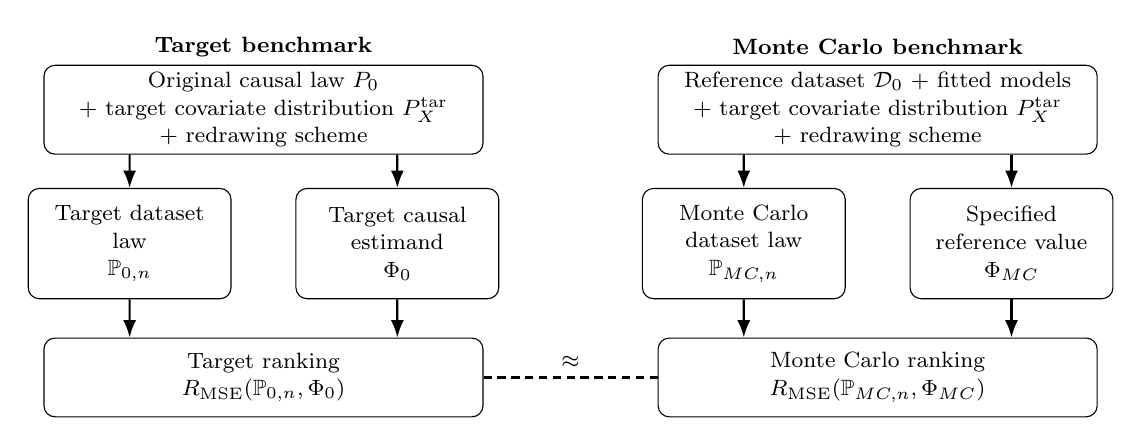
\begin{tikzpicture}[
    box/.style={
        draw,
        rounded corners,
        align=center,
        font=\fontsize{8pt}{10pt}\selectfont,
        text width=2.4cm,
        minimum height=0.75cm,
        inner sep=2.5pt,
        execute at begin node=\setlength{\parskip}{0pt}
    },
    widebox/.style={box, text width=5.4cm},
    componentbox/.style={box, minimum height=1.4cm},
    finalbox/.style={widebox, minimum height=1.0cm},
    heading/.style={font=\fontsize{8pt}{10pt}\selectfont\bfseries, align=center},
    arrow/.style={-{Latex[length=2.2mm]}, thick}
]

% The two processes have the same structure: inputs, law and target, performance.
\node[heading] at (0,0.8) {Target benchmark};
\node[heading] at (7.8,0.8) {Monte Carlo benchmark};

\node[widebox] (original) at (0,0) {Original causal law \(P_0\)\\ + target covariate distribution \(P_X^{\mathrm{tar}}\)\\ + redrawing scheme};
\node[widebox] (design) at (7.8,0) {Reference dataset \(\mathcal D_0\) + fitted models\\ + target covariate distribution \(P_X^{\mathrm{tar}}\)\\ + redrawing scheme};

\node[componentbox] (redraw) at (-1.7,-1.7) {Target dataset\\ law\\ \(\mathbb P_{0,n}\)};
\node[componentbox] (estimand) at (1.7,-1.7) {Target causal\\ estimand\\ \(\Phi_0\)};
\node[componentbox] (mclaw) at (6.1,-1.7) {Monte Carlo\\ dataset law\\ \(\mathbb P_{MC,n}\)};
\node[componentbox] (mcvalue) at (9.5,-1.7) {Specified\\ reference value\\ \(\Phi_{MC}\)};

\node[finalbox] (targetbenchmark) at (0,-3.4) {Target ranking\\ \(R_{\mathrm{MSE}}(\mathbb P_{0,n},\Phi_0)\)};
\node[finalbox] (mcbenchmark) at (7.8,-3.4) {Monte Carlo ranking\\ \(R_{\mathrm{MSE}}(\mathbb P_{MC,n},\Phi_{MC})\)};

\draw[arrow] ([xshift=-1.7cm]original.south) -- (redraw.north);
\draw[arrow] ([xshift=1.7cm]original.south) -- (estimand.north);
\draw[arrow] ([xshift=-1.7cm]design.south) -- (mclaw.north);
\draw[arrow] ([xshift=1.7cm]design.south) -- (mcvalue.north);

\draw[arrow] (redraw.south) -- ([xshift=-1.7cm]targetbenchmark.north);
\draw[arrow] (estimand.south) -- ([xshift=1.7cm]targetbenchmark.north);
\draw[arrow] (mclaw.south) -- ([xshift=-1.7cm]mcbenchmark.north);
\draw[arrow] (mcvalue.south) -- ([xshift=1.7cm]mcbenchmark.north);

\draw[densely dashed, thick] (targetbenchmark.east)
    -- node[above, font=\fontsize{8pt}{10pt}\selectfont] {\(\approx\)} (mcbenchmark.west);
\end{tikzpicture}

\captionsetup{font=normalsize}
\caption{Conceptual exercise: target and Monte Carlo benchmarks. Ideally, the study should approximate the performance that would be obtained with access to the original objects.}
\label{fig:conceptual_exercise}
\end{figure*}



\subsection{Outcome-model approximation}
\label{sec:outcome-model-approximation}

Most EMCS use \(\mathcal D_0\) to fit an outcome model conditional on covariates and treatment, \(\widehat P_{MC}(Y\mid X,A)\approx P_{0}(Y\mid X,A)\). This model is then employed to construct both \(\mathbb P_{MC,n}\) and \(\Phi_{MC}\). For the same target covariate distribution \(P_X^{\mathrm{tar}}\), replacing the conditional means in Equation~\eqref{eq:identified-conditional-mean} with those of the fitted model gives
\begin{equation}
\begin{aligned}
\widehat\mu_{MC,a}(x)
&:=\mathbb E_{\widehat P_{MC}}[Y\mid X=x,A=a],\\
\Phi_{MC}
&:=\mathbb E_{X\sim P_X^{\mathrm{tar}}}
\left[\widehat\mu_{MC,1}(X)-\widehat\mu_{MC,0}(X)\right].
\end{aligned}
\label{eq:simulator-induced-estimand}
\end{equation}
Therefore, the fitted model affects both the behavior of estimators and the estimand against which they are compared. We can write the fitted conditional mean as
\[
\widehat\mu_{MC,a}(x)=\mu_{0,a}(x)+r_a(x),
\]
where \(r_a\) captures model misspecification and finite-sample estimation error and is fixed once the simulator has been fitted. Subtracting Equation~\eqref{eq:identified-conditional-mean} from Equation~\eqref{eq:simulator-induced-estimand}, with the same target covariate distribution \(P_X^{\mathrm{tar}}\), gives
\begin{equation}
\Phi_{MC}-\Phi_0
=\mathbb E_{X\sim P_X^{\mathrm{tar}}}\left[r_1(X)-r_0(X)\right].
\label{eq:simulator-estimand-shift}
\end{equation}
Errors in the two fitted conditional means can cancel when averaged over the target covariate distribution: \(\Phi_{MC}=\Phi_0\) can hold even when those means are misspecified.

Model alignment bias can arise when an estimator \(e_1\) represents \(\widehat\mu_{MC,a}\) well, whereas another estimator \(e_2\) better approximates \(\mu_{0,a}\). Their MSE ordering can consequently reverse:
\[
\begin{aligned}
\mathrm{MSE}(e_2;\mathbb P_{0,n},\Phi_0)
&<\mathrm{MSE}(e_1;\mathbb P_{0,n},\Phi_0),\\
\mathrm{MSE}(e_2;\mathbb P_{MC,n},\Phi_{MC})
&>\mathrm{MSE}(e_1;\mathbb P_{MC,n},\Phi_{MC}).
\end{aligned}
\]
Such a reversal can occur even when the average contrast in Equation~\eqref{eq:simulator-estimand-shift} is zero, since the fitted outcome structure may alter estimator-specific bias and variance. Preserving the benchmark value therefore does not ensure ranking fidelity as defined in Equation~\eqref{eq:ranking-preservation}.

Matching conditional means alone also does not determine estimator performance. A simulator may fail to reproduce heteroskedasticity; with non-iid errors, even matching each unit's conditional outcome distribution does not ensure that it reproduces the joint outcome law across units. Both discrepancies can affect estimator variance, MSE, and rankings while preserving the reference value.

\subsection{The SACTE estimand and fixed-design benchmarks}
\label{sec:fixed-design-sacte}

Taking the target covariate distribution to be the empirical distribution described in Section~\ref{sec:causal-framework} for a reference sample of size \(n=n_0\) gives the SACTE,
\begin{equation}
\Phi_0^{\mathrm{SACTE}}
=\frac1n\sum_{i=1}^n
\left[\mu_{0,1}(X_i)-\mu_{0,0}(X_i)\right].
\label{eq:sacte}
\end{equation}
This estimand averages conditional treatment effects over the realized covariate profiles, rather than over the population covariate distribution. It therefore requires the conditional outcome means at these profiles but no additional population covariate model. \authorcite{imbensNonparametricEstimationAverage2004} discusses this estimand under the name conditional average treatment effect; we use SACTE to distinguish it from the now-common use of CATE for the pointwise contrast \(\mathbb E[Y(1)-Y(0)\mid X=x]\).

Fixing the reference covariates defines a natural redrawing scheme for this estimand, while treatment assignments can either be redrawn or held fixed, depending on the inferential aim of the simulation. In this paper, we focus on the case where the realized treatment vector is fixed and only outcomes are redrawn conditional on \((X,A)\). The resulting benchmark evaluates performance for the particular covariate--treatment configuration observed in the reference sample. Thus, both the target law \(\mathbb P_{0,n}\) and the simulator law \(\mathbb P_{MC,n}\) will produce the same covariate--treatment configuration, while their outcome mechanisms and corresponding SACTEs may differ. This choice isolates outcome-model approximation bias from approximation of the covariate and treatment distributions and reduces the modeling choices and computational load.

An interesting consequence of targeting the SACTE under this conditional design is that we can retain the observed covariate--treatment pairs without introducing additional bias distortion for propensity-score-based estimation. \authorcite{shawCautionaryNotePlasmode2026} show that the \emph{Sample Treatment} redrawing scheme, which jointly bootstraps $(X,A)$ and generates outcomes, can misrepresent IPW bias relative to the iid target $\mathbb P_{0,n}=(P_0)^n$, even with correctly specified outcome models. This is because its induced law can only generate a single treatment value at unique reference covariate profiles, even when $P_0$ satisfies positivity as in Equation~\eqref{eq:positivity}. Instead, the \emph{Generate Treatment} scheme, which generates treatment from a propensity model, avoids this problem.

This issue does not arise in our fixed-design comparison. For a general IPW estimator, write
\[
\widehat\Phi_{\mathrm{IPW}}=\sum_{i=1}^n w_iY_i,
\]
where \(w_i\) are signed weights determined by covariates, treatment, and estimated propensity scores (see Appendix~\ref{app:ipw} for a description of our specification). In our fixed-design SACTE benchmark, both the target and simulator laws retain the same \((X,A)\). Holding the propensity-fitting folds and randomization fixed gives identical weights under both benchmarks; assume both treatment groups are nonempty and estimated propensity scores lie strictly between zero and one. With conditional outcome means \(\mu_{0,A_i}(X_i)\) and \(\widehat\mu_{MC,A_i}(X_i)\), the difference between conditional biases is
\[
\begin{aligned}
\operatorname{Bias}_{MC}-\operatorname{Bias}_0
&=\sum_{i=1}^n w_i[\widehat\mu_{MC,A_i}(X_i)-\mu_{0,A_i}(X_i)]\\
&\quad-(\Phi_{MC}-\Phi_0)\\
&=\sum_{i=1}^n w_i r_{A_i}(X_i)
-\frac1n\sum_{i=1}^n[r_1(X_i)-r_0(X_i)].
\end{aligned}
\]
Each bias is relative to its corresponding SACTE. The bias discrepancy arises from outcome-model approximation error and tends to zero as the fitted conditional means approach the target means, even with misspecified propensity scores. Because the target law \(\mathbb P_{0,n}\) is itself defined conditionally on the observed \((X,A)\), retaining these values in \(\mathbb P_{MC,n}\) introduces no mismatch in the covariate--treatment configuration. In the Sample Treatment scheme, by contrast, the simulation law replaces the nondegenerate treatment mechanism of an iid target with a degenerate empirical one.

% !TeX root = Master.tex
\section{Simulation design}
\label{sec:simulation-design}

To illustrate the framework and gain evidence on the empirical performance of EMCS in controlled scenarios, we conduct a simulation study with particular attention to the model-alignment concern raised in Section~\ref{sec:framework}. We use two established collections of benchmark designs: the 2017 Atlantic Causal Inference Conference (ACIC) designs presented by \authorcite{hahnAtlanticCausalInference2019}, which use covariates from the Infant Health and Development Program, and the fully synthetic, nonlinear designs of \authorcite{nieQuasioracleEstimationHeterogeneous2021} (N\&W).

We consider 12 settings: four error structures for ACIC 2017 and four DGPs (A--D) for N\&W, each at two sample sizes. We index these settings, including sample size, by \(g\in\mathcal G\). Each design defines a reference-dataset law \(\mathbb G_n^{g}\), which we call its \emph{generator}. Throughout the paper, we use \emph{generator} to refer to \(\mathbb G_n^{g}\) and, by extension, sometimes to the full design \(g\). For each \(g\), we draw from this law to generate \(M=100\) reference datasets that play the role of \(\mathcal D_0\) in Equation~\eqref{eq:observed-data-causal-law}:
\[
\mathcal D^{g,m}=\{(X_i^{g,m},A_i^{g,m},Y_i^{g,m})\}_{i=1}^n
\sim\mathbb G_n^{g},
\qquad m=1,\dots,M.
\]

Our objective is to mimic an applied case study in which, given a reference dataset \(\mathcal D^{g,m}\), a researcher sets up an EMCS to rank a collection of causal estimators \(\mathcal E\) targeting the SACTE. We choose a redrawing scheme that conditions on the reference covariates and treatment, so variability comes only from redrawing outcomes. We fit conditional outcome simulators, indexed by \(s\in\mathcal S\), to each reference dataset.

Because the true outcome-generating mechanism is known, the target benchmark \((\mathbb P_{0,n}^{g,m},\Phi_0^{g,m})\) serves as an oracle for evaluating the fitted-simulator benchmarks under the same redrawing scheme. The following subsections describe the generators, simulators, and causal estimators; Section~\ref{sec:benchmarking-procedure} details the benchmark construction and study workflow.

\subsection{The generators}
\label{sec:generators}

To define the dataset laws \(\mathbb G_n^{g}\) used to generate the reference datasets, we follow the ACIC 2017 and N\&W designs. The ACIC 2017 designs \cite{hahnAtlanticCausalInference2019} reuse covariates from the Infant Health and Development Program (IHDP) and impose synthetic treatment and outcome mechanisms on that empirical covariate distribution. The ACIC designs fix the observed covariates and generate new datasets by drawing treatments and outcomes conditional on these fixed covariates according to the design's propensity-score and outcome models. We focus on settings with strong effects and high confounding and on the four error structures: additive homoskedastic iid, non-additive, group-correlated, and heteroskedastic. This allows us to assess how different error structures affect the ability of EMCS benchmarks to preserve estimator performance and rankings.

Although ACIC 2017 does not specify a population model for the covariates, its outcome mechanism suffices to compute the SACTE in Equation~\eqref{eq:sacte} over the fixed reference covariates. Together with its treatment mechanism and the fixed covariates, it also determines the reference-dataset law \(\mathbb G_n^{g}\).

By contrast, the N\&W designs \cite{nieQuasioracleEstimationHeterogeneous2021}
are fully synthetic: covariates, treatments, and outcomes are generated from nonlinear specifications. We use the four DGPs (A--D) proposed there with covariate dimension $d=6$. We run the N\&W DGPs at one of the original sample sizes from the paper, $n=1000$, and additionally at $n=4302$ to match the ACIC 2017 sample size; this lets us compare design families directly and assess the effect of sample size on simulator fidelity.

Thus, \(\Phi_0^{g,m}\) is constant across reference datasets \(m\) for ACIC 2017, where covariates are fixed, but can vary across reference datasets for the N\&W designs, where covariates are redrawn. In N\&W design C, however, the constant conditional treatment effect makes the SACTE constant as well.

Appendix~\ref{app:generators} shows the implemented ACIC and N\&W specifications.

\subsection{The simulators}

The simulators we study can be classified into two broad classes. Both define stochastic conditional outcome distributions.

\noindent\textbf{Conditional-mean simulators:}
These simulators estimate a conditional mean function,
\[
\widehat\mu_s(x,a)
\approx
\mathbb E[Y\mid X=x,A=a],
\]
and treatment-specific heteroskedastic standard-deviation functions \(\widehat\sigma_{s,a}(x)\). For simulator \(s\), the \(k\)-th synthetic outcome is generated as
\[
\begin{aligned}
\widetilde Y_{i,s}^{g,m,k}
&= A_i^{g,m}\left\{\widehat\mu_{s,1}^{g,m}(X_i^{g,m})
+ \widehat\sigma_{s,1}^{g,m}(X_i^{g,m})\varepsilon_{i1}^{(k)}\right\} \\[-2pt]
&+ \bigl(1-A_i^{g,m}\bigr)\left\{\widehat\mu_{s,0}^{g,m}(X_i^{g,m})
+ \widehat\sigma_{s,0}^{g,m}(X_i^{g,m})\varepsilon_{i0}^{(k)}\right\}.
\end{aligned}
\]
Here, \(\varepsilon_{ia}^{(k)}\overset{\mathrm{iid}}{\sim}\mathcal N(0,1)\) for \(a\in\{0,1\}\).
Thus, the observed treatment selects the fitted conditional mean and corresponding heteroskedastic noise scale. The simulator comprises these fitted functions and the Gaussian error distribution; labels such as GB or RF identify the learner family used to construct it. To estimate \(\widehat\mu_s\) and \(\widehat\sigma_s\), we employ OLS with squared terms and pairwise interactions between variables (OLS2), gradient boosting (GB), random forest (RF), and neural-network (NN) models.

\noindent\textbf{Generative simulators:}
This type of simulator aims to approximate the full conditional distribution directly, drawing independently across units: \(\widetilde Y_{i,s}^{g,m,k}\sim\widehat P_s(\cdot\mid X_i^{g,m},A_i^{g,m})\). We include a conditional Wasserstein generative adversarial network (WGAN) with gradient penalty, as introduced by \authorcite{gulrajaniImprovedTrainingWasserstein2017}. We follow the approach of \authorcite{atheyUsingWassersteinGenerative2024} and use a very similar architecture, but while they fit two models, one to generate \(X_i\) conditional on \(A_i\) and another to generate outcomes conditional on \(X_i,A_i\), we only evaluate the latter. Still, our results are informative for broader designs that generate covariates and treatment, since these designs must also reproduce the conditional outcome distribution. Failure at this stage would compromise the resulting simulation study.

The fitted WGAN defines a conditional outcome distribution implicitly, without an explicit conditional mean function. At each fixed reference covariate vector, we approximate its treatment-specific conditional means by averaging 10,000 generated outcomes under each treatment. Averaging the resulting mean contrasts over the reference covariates gives a Monte Carlo approximation to its induced SACTE in Equation~\eqref{eq:simulator-induced-estimand}.

Additional implementation details for the simulator models are provided in Appendix~\ref{app:simulators}.

\subsection{Causal estimators}

We compare a set of estimators \(\mathcal E\) that are commonly used in the causal-inference literature and that involve fitting outcome and/or propensity score models. Although these methods are often used as ATE estimators, the same point-estimation formulas apply to the SACTE. \authorcite{imbensNonparametricEstimationAverage2004} shows that efficient estimators of the population average treatment effect can also be interpreted as estimators of the corresponding sample average treatment effect, with the same point estimator but a smaller asymptotic variance when inference is conditional on the realized sample. The choice of the SACTE therefore determines the benchmark value against which bias and MSE are computed. The construction of the point estimates is unchanged, but if we were estimating standard errors or coverage, we would need variance estimators appropriate for inference conditional on the realized covariates.

For outcome regression, we use ordinary least squares with squared terms and pairwise interactions between variables (OLS2), gradient boosting (GB), random forests (RF), and neural networks (NN), with the same conditional-mean specifications as the corresponding simulators to induce model alignment. Following \authorcite{chernozhukovDoubleDebiasedMachine2018}, these outcome models are fitted using five-fold cross-fitting, which constitutes a difference in fitting procedure relative to their simulator counterparts. For propensity score estimation, we use a gradient-boosting classifier, also fitted using five-fold cross-fitting, selected after comparing several classifiers. The GB, RF, and NN outcome models and the GB classifier are implemented in \texttt{scikit-learn}.

We use these models in G-computation (G-comp), normalized inverse probability weighting (IPW) \cite{luncefordStratificationWeightingPropensity2004}, augmented inverse probability weighting (AIPW) \cite{bangDoublyRobustEstimation2005}, and targeted maximum likelihood estimation (TMLE) \cite{vanderlaanTargetedMaximumLikelihood2006}. G-comp labels identify the outcome model, while the AIPW and TMLE labels give the propensity model followed by the outcome model; for example, GB--RF AIPW uses GB propensity scores and RF outcome regression. GB IPW uses only the GB propensity model. We also include Bayesian causal forest (BCF G-comp) \cite{hahnBayesianRegressionTree2020}, implemented in \texttt{stochtree}, and linear regression with additive effects (OLS1). We count OLS1 as aligned with OLS2 because of their similar specifications. Table~\ref{tab:estimators} summarizes the estimators, labels, nuisance models, and aligned simulators. Appendix~\ref{app:estimators} provides the estimator formulas and implementation details, including the in-sample propensity fit used by BCF.

\begin{table*}[!t]
\centering
\caption{Estimator summary with associated labels, nuisance models, and aligned simulators.}
\label{tab:estimators}
{

\begin{tabular}{p{3.2cm}llll}
\toprule
Estimator class & Estimator label & Outcome model & Propensity model & Aligned simulator \\
\midrule
OLS (linear effects) & OLS1 & OLS1 & -- & OLS2 \\
\midrule
\multirow{4}{3.2cm}{G-computation} & OLS2 G-comp & OLS2 & -- & OLS2 \\
& GB G-comp & GB & -- & GB \\
& RF G-comp & RF & -- & RF \\
& NN G-comp & NN & -- & NN \\
\midrule
Inverse probability weighting & GB IPW & -- & GB & -- \\
\midrule
\multirow{4}{3.2cm}{Augmented inverse probability weighting} & GB--OLS2 AIPW & OLS2 & GB & OLS2 \\
& GB--GB AIPW & GB & GB & GB \\
& GB--RF AIPW & RF & GB & RF \\
& GB--NN AIPW & NN & GB & NN \\
\midrule
\multirow{4}{3.2cm}{Targeted maximum likelihood estimation} & GB--OLS2 TMLE & OLS2 & GB & OLS2 \\
& GB--GB TMLE & GB & GB & GB \\
& GB--RF TMLE & RF & GB & RF \\
& GB--NN TMLE & NN & GB & NN \\
\midrule
Bayesian causal forest & BCF G-comp & BCF & GB & -- \\
\bottomrule
\end{tabular}
}
\end{table*}



% !TeX root = Master.tex
\section{Study workflow}
\label{sec:benchmarking-procedure}

The generation pipeline proceeds from the chosen design to simulated datasets and estimates; the evaluation pipeline computes estimation errors and aggregates them into performance summaries and rankings.

\subsection{Generation pipeline}

We organize generation into six levels, introducing indices for the design, reference dataset, simulator, Monte Carlo draw, and estimator.

\medskip
\noindent\textbf{Level 0. Choose study components:} We fix the set of designs \(\mathcal G\), the set of simulator specifications \(\mathcal S\), and the set of estimators \(\mathcal E\). For ACIC 2017-style designs, the reference covariates are also fixed as part of the design.

\medskip
\noindent\textbf{Level 1. Select a generator:} We select a design \(g\in\mathcal G\) and construct its generator \(\mathbb G_n^{g}\).

\medskip
\noindent\textbf{Level 2. Generate reference datasets:} We draw \(M=100\) reference datasets \(\mathcal D^{g,m}\) from \(\mathbb G_n^{g}\), each playing the role of the reference dataset \(\mathcal D_0\) in Equation~\eqref{eq:observed-data-causal-law}.

\medskip
\noindent\textbf{Level 3. Construct benchmarks:} For each reference dataset \(\mathcal D^{g,m}\), we fit all simulators \(s\in\mathcal S\), yielding the conditional outcome laws \(\widehat P_s^{\,g,m}(\cdot\mid X,A)\). Applying Equation~\eqref{eq:simulator-induced-estimand} to the reference covariates gives the simulator-specific benchmark:
\begin{equation}
\begin{gathered}
\mathbb P_{s,n}^{g,m}:\quad
\bigl(X_i,A_i\bigr)
=\bigl(X_i^{g,m},A_i^{g,m}\bigr),\\
Y_i\sim\widehat P_s^{\,g,m}\bigl(\cdot\mid X_i,A_i\bigr),\\
\Phi_s^{g,m}
=
\frac1n
\sum_{i=1}^n
\left[
\widehat\mu_{s,1}^{\,g,m}(X_i^{g,m})
-
\widehat\mu_{s,0}^{\,g,m}(X_i^{g,m})
\right].
\end{gathered}
\label{eq:simulator-specific-benchmark}
\end{equation}

Using the design's true outcome-generating mechanism while keeping the reference covariates and treatment assignments fixed gives the target benchmark \(\bigl(\mathbb P_{0,n}^{g,m},\Phi_0^{g,m}\bigr)\). Notice that the target dataset law \(\mathbb P_{0,n}^{g,m}\) differs from the original generator \(\mathbb G_n^{g}\) used to produce reference datasets: their conditional outcome models are the same, but while \(\mathbb P_{0,n}^{g,m}\) redraws only outcomes, the ACIC generators redraw treatment and the N\&W generators redraw both covariates and treatment.

\medskip
\noindent\textbf{Level 4. Generate Monte Carlo datasets:} We generate \(K=1000\) datasets from each fitted-simulator benchmark and from the target benchmark:
\[
\begin{gathered}
\widetilde{\mathcal D}_{s,n}^{g,m,k}
\overset{\mathrm{iid}}{\sim}\mathbb P_{s,n}^{g,m},
\qquad s\in\mathcal S,\\
\mathcal D_{0,n}^{g,m,k}
\overset{\mathrm{iid}}{\sim}\mathbb P_{0,n}^{g,m},
\qquad k=1,\dots,K.
\end{gathered}
\]

\medskip
\noindent\textbf{Level 5. Apply causal estimators:} Each estimator \(e\in\mathcal E\) is applied to every simulator-induced and target-benchmark dataset, yielding \(\widehat\Phi_{e}^{\,g,m,s,k}\).

\begin{figure*}[!t]
\centering
\makebox[\textwidth][c]{%
\pgfdeclarelayer{continuations}
\pgfsetlayers{continuations,main}
\begin{tikzpicture}[
    x=0.82cm, y=0.68cm,
    every node/.style={font=\fontsize{7pt}{9pt}\selectfont},
    box/.style={
        draw,
        rounded corners,
        align=center,
        minimum width=4.9cm,
        minimum height=0.75cm,
        inner sep=2.5pt,
        text width=4.8cm
    },
    widebox/.style={box, minimum width=4.9cm, text width=4.8cm},
    colbox/.style={box, minimum width=4.9cm, text width=4.8cm},
    simbox/.style={box, minimum width=4.9cm, text width=4.8cm, minimum height=1.15cm},
    obsbox/.style={box, minimum width=4.9cm, text width=4.8cm, inner sep=2pt},
    lvl/.style={
        align=right, text width=3cm, anchor=east,
        font=\fontsize{8pt}{10pt}\selectfont\bfseries, execute at begin node={\hyphenpenalty=10000\relax}
    },
    arr/.style={-{Stealth[length=1.3mm]}, semithick},
    continuation/.style={-{Stealth[length=1.3mm]}, draw=black, densely dotted, semithick}
]

% Study design
\node[widebox] (design) at (2,0) {Study design\\ \(\mathcal G,\mathcal S,\mathcal E\)};

% Original dataset laws
\node[colbox, anchor=north] (law1) at ([xshift=-5.166cm,yshift=-0.5cm]design.south) {\(\mathbb G_n^{g-1}\)};
\node[colbox, anchor=north] (law2) at ([xshift=0cm,yshift=-0.5cm]design.south) {\(\mathbb G_n^{g}\)};
\node[colbox, anchor=north] (law3) at ([xshift=5.166cm,yshift=-0.5cm]design.south) {\(\mathbb G_n^{g+1}\)};

\draw[arr] ([xshift=1.0cm]design.south west) -- (law1.north);
\draw[arr] (design) -- (law2.north);
\draw[arr] ([xshift=-1.0cm]design.south east) -- (law3.north);

% Reference datasets
\node[obsbox, anchor=north] (obs1) at ([xshift=-5.166cm,yshift=-0.5cm]law2.south) {\(\mathcal D^{g,m-1}\)};
\node[obsbox, anchor=north] (obs2) at ([xshift=0cm,yshift=-0.5cm]law2.south) {\(\mathcal D^{g,m}\)};
\node[obsbox, anchor=north] (obs3) at ([xshift=5.166cm,yshift=-0.5cm]law2.south) {\(\mathcal D^{g,m+1}\)};

\draw[arr] ([xshift=1.0cm]law2.south west) -- (obs1.north);
\draw[arr] (law2) -- (obs2.north);
\draw[arr] ([xshift=-1.0cm]law2.south east) -- (obs3.north);

% Simulator-induced benchmark objects
\node[simbox, anchor=north] (sim1) at ([xshift=-5.166cm,yshift=-0.5cm]obs2.south) {
    \(\widehat P_{s-1}^{\,g,m}(\cdot\mid X,A)\)\\[-1pt]
    \(\downarrow\)\\[-1pt]
    \(\bigl(\mathbb P_{s-1,n}^{g,m},\Phi_{s-1}^{g,m}\bigr)\)
};
\node[simbox, anchor=north] (sim2) at ([xshift=0cm,yshift=-0.5cm]obs2.south) {
    \(\widehat P_s^{\,g,m}(\cdot\mid X,A)\)\\[-1pt]
    \(\downarrow\)\\[-1pt]
    \(\bigl(\mathbb P_{s,n}^{g,m},\Phi_s^{g,m}\bigr)\)
};
\node[simbox, anchor=north] (sim3) at ([xshift=5.166cm,yshift=-0.5cm]obs2.south) {
    \(\widehat P_{s+1}^{\,g,m}(\cdot\mid X,A)\)\\[-1pt]
    \(\downarrow\)\\[-1pt]
    \(\bigl(\mathbb P_{s+1,n}^{g,m},\Phi_{s+1}^{g,m}\bigr)\)
};

\draw[arr] ([xshift=1.0cm]obs2.south west) -- (sim1.north);
\draw[arr] (obs2) -- (sim2.north);
\draw[arr] ([xshift=-1.0cm]obs2.south east) -- (sim3.north);

% Synthetic datasets
\node[colbox, anchor=north] (syn1) at ([xshift=-5.166cm,yshift=-0.5cm]sim2.south) {\(\widetilde{\mathcal D}_{s,n}^{g,m,k-1}\)};
\node[colbox, anchor=north] (syn2) at ([xshift=0cm,yshift=-0.5cm]sim2.south) {\(\widetilde{\mathcal D}_{s,n}^{g,m,k}\)};
\node[colbox, anchor=north] (syn3) at ([xshift=5.166cm,yshift=-0.5cm]sim2.south) {\(\widetilde{\mathcal D}_{s,n}^{g,m,k+1}\)};

\draw[arr] ([xshift=1.0cm]sim2.south west) -- (syn1.north);
\draw[arr] (sim2) -- (syn2.north);
\draw[arr] ([xshift=-1.0cm]sim2.south east) -- (syn3.north);

% Estimators / Phi estimates
\node[colbox, anchor=north] (est1) at ([xshift=-5.166cm,yshift=-0.5cm]syn2.south) {\(\widehat\Phi_{e_{j-1}}^{\,g,m,s,k}\)};
\node[colbox, anchor=north] (est2) at ([xshift=0cm,yshift=-0.5cm]syn2.south) {\(\widehat\Phi_{e_j}^{\,g,m,s,k}\)};
\node[colbox, anchor=north] (est3) at ([xshift=5.166cm,yshift=-0.5cm]syn2.south) {\(\widehat\Phi_{e_{j+1}}^{\,g,m,s,k}\)};

\draw[arr] ([xshift=1.0cm]syn2.south west) -- (est1.north);
\draw[arr] (syn2) -- (est2.north);
\draw[arr] ([xshift=-1.0cm]syn2.south east) -- (est3.north);

\coordinate (labelaxis) at (-7.7,0);
% Level labels
\node[lvl] at (design.center -| labelaxis) {Level 0. Choose study components:};
\node[lvl] at (law2.center -| labelaxis) {Level 1. Select a generator:};
\node[lvl] at (obs2.center -| labelaxis) {Level 2. Generate reference datasets:};
\node[lvl] at (sim2.center -| labelaxis) {Level 3. Construct benchmarks:};
\node[lvl] at (syn2.center -| labelaxis) {Level 4. Generate Monte Carlo datasets:};
\node[lvl] at (est2.center -| labelaxis) {Level 5. Apply causal estimators:};

% Background fans suggest the omitted descendants of each side branch.
% Their endpoints remain in the gap between levels, without reaching a box.
\begin{pgfonlayer}{continuations}
\foreach \branch in {law1,law3,obs1,obs3,sim1,sim3,syn1,syn3} {
    \draw[continuation] ([xshift=1cm]\branch.south west) -- ++(-1.45,-0.30);
    \draw[continuation] (\branch.south) -- ++(0,-0.30);
        \draw[continuation] ([xshift=-1cm]\branch.south east) -- ++(1.45,-0.30);
}
\end{pgfonlayer}

\end{tikzpicture}
}
\caption{Generation pipeline. Dotted arrows indicate continuation of the side branches through omitted repetitions. The same redrawing and estimation steps are applied to the target benchmark \((\mathbb P_{0,n}^{g,m},\Phi_0^{g,m})\), using the true conditional outcome mechanism.}
\label{fig:generation_pipeline}
\end{figure*}


\subsection{Evaluation pipeline}

The evaluation pipeline moves from higher to lower levels, aggregating estimates into summaries:

\medskip

\noindent\textbf{Level 5. Compute estimation errors:} For each estimate under a fitted simulator \(s\in\mathcal S\), we compute the error relative to its benchmark estimand,

\[
\mathrm{Err}_{e}^{\,g,m,s,k}
=
\widehat{\Phi}_{e}^{\,g,m,s,k}
-
\Phi_s^{g,m}.
\]
For the target benchmark, \(\mathrm{Err}_{e}^{\,g,m,0,k}=\widehat\Phi_{e}^{\,g,m,0,k}-\Phi_0^{g,m}\).

\medskip

\noindent\textbf{Level 4. Summarize estimator performance:} For each fitted or target benchmark, the \(K\) estimation errors give the Monte Carlo MSE, \(\widehat{\mathrm{MSE}}^{g,m,s}(e)=K^{-1}\sum_{k=1}^K(\mathrm{Err}_e^{g,m,s,k})^2\), with \(s=0\) for the target benchmark.

\medskip

\noindent\textbf{Level 3. Rank estimators by MSE:} We rank the estimators by MSE under each simulator-induced and target benchmark. These are the empirical counterparts of the rankings in Equation~\eqref{eq:ranking-preservation}. We denote the rankings estimated from \(K\) draws by \(\widehat R_{\mathrm{MSE}}^{\,g,m,s}\) under simulator \(s\) and \(\widehat R_{\mathrm{MSE}}^{\,g,m,0}\) under the target benchmark. Rank 1 denotes the lowest MSE. The target-benchmark ranking is used as the comparator in the following calculations.

\medskip

\noindent\textbf{Level 2. Compare rankings with target:} For each reference dataset \(m\), we measure ranking fidelity by \(\rho^{g,m,s}\), the Spearman correlation between the estimator rankings under fitted simulator \(s\) and the target benchmark, i.e., Pearson correlation applied to the ranks.

To assess model alignment, we repeat this computation after excluding from both rankings the estimators aligned with simulator \(s\), denoting the result by \(\rho_{\mathrm{excl}}^{g,m,s}\). For each reference dataset \(m\) and simulator \(s\), we also compute \emph{rank promotion}, \(\mathrm{Prom}^{g,m,s}(e)\): estimator \(e\)'s position in the target-benchmark ranking minus its position in \(\widehat R_{\mathrm{MSE}}^{\,g,m,s}\). Positive mean promotion indicates a tendency to rank estimators higher under the simulator than under the target benchmark. For a simulator with aligned estimators, we consider the G-comp, AIPW, and TMLE estimators using its outcome learner. We also report absolute rank shifts, given by the absolute values of these promotions, and compare both measures with the corresponding averages over non-aligned estimators (Rest). We use \(\boldsymbol{\mathrm{Prom}}^{g,m,s}\) to denote the vector collecting promotions and absolute rank shifts for these three estimators.

For each reference dataset, we also aggregate the five simulator rankings by averaging each estimator's MSE rank across simulators and ranking these averages. In the alignment-excluded version, each estimator's average uses only simulators with which it is not aligned; all estimators remain in the aggregate ranking.

We also compute the estimand gap \(\Delta\Phi_s^{g,m}=\Phi_s^{g,m}-\Phi_0^{g,m}\) to examine whether smaller absolute gaps accompany higher ranking fidelity.

We ask whether simulator-based selection improves on using the associated G-comp estimator. For each reference dataset $m$ and simulator $s$, we compare three rules, each selecting an estimator $\widehat e_r^{g,m,s}\in\mathcal E$:
\begin{enumerate}
    \item \emph{G-comp}: the associated G-computation estimator, chosen without consulting the simulator ranking;
    \item \emph{All}: the estimator minimizing simulator MSE among all 15 estimators;
    \item \emph{Excl.}: the estimator minimizing simulator MSE among non-aligned estimators.
\end{enumerate}
Following \authorcite{advaniMostlyHarmlessSimulations2019}, \emph{relative MSE regret} measures percentage excess target-benchmark MSE over the best of all 15 estimators:
\begin{equation}
\mathrm{Reg}^{g,m}(e)
=100\left\{
\frac{\widehat{\mathrm{MSE}}^{g,m,0}(e)}
{\min_{j\in\mathcal E}\widehat{\mathrm{MSE}}^{g,m,0}(j)}-1
\right\}.
\label{eq:relative-mse-regret}
\end{equation}
Thus, 0 means matching the target-best MSE and 100 means twice that MSE. The vector \(\boldsymbol{\mathrm{Reg}}^{g,m,s}\) collects the regrets of the G-comp, All, and Excl. rules, in that order. Table~\ref{tab:gcomp-selection} reports the mean regret for each rule over the $M=100$ reference datasets; lower values are better. WGAN is omitted because it has no associated G-comp estimator to serve as the default.

We assess the similarity between real and synthetic outcomes using the Wasserstein-1 (\(W_1\)), Kolmogorov--Smirnov (KS), and energy distances. Each distance is averaged over the \(K\) Monte Carlo datasets; the vector \(\boldsymbol d^{g,m,s}\) collects these values in the order \(W_1\), KS, energy. For each reference dataset, we compute the Pearson correlation between distance and ranking fidelity across the five simulators, then average these correlations within each setting. Appendix~\ref{app:distances} gives further details.

\medskip

\noindent\textbf{Level 1. Average comparison metrics:} For each design \(g\) and simulator \(s\), we average across the \(M\) reference datasets to obtain the mean rank correlations \(\bar\rho^{g,s}\) and \(\bar\rho_{\mathrm{excl}}^{g,s}\), the mean absolute estimand gap \(\overline{|\Delta\Phi_s|}^{g}=M^{-1}\sum_{m=1}^{M}|\Delta\Phi_s^{g,m}|\), the mean promotions and absolute rank shifts \(\overline{\boldsymbol{\mathrm{Prom}}}^{g,s}\), the mean regrets \(\overline{\boldsymbol{\mathrm{Reg}}}^{g,s}\), and the mean distances \(\overline{\boldsymbol d}^{g,s}=M^{-1}\sum_{m=1}^{M}\boldsymbol d^{g,m,s}\). Bars denote means over reference datasets. Simulators are ranked by their mean rank correlations.

\medskip

\noindent\textbf{Level 0. Draw general conclusions:} Finally, results are compared across DGPs to assess whether conclusions regarding ranking fidelity, simulator performance, and model alignment are consistent across the different data-generating processes.

\medskip

This evaluation pipeline is summarized in Figure~\ref{fig:evaluation_pipeline}.

Code and numerical results for reproducing the analyses are available in the accompanying repository (see \hyperref[sec:code-data-availability]{Code and Data Availability}).

\begin{figure*}[!t]
\centering
\makebox[\textwidth][c]{%
\pgfdeclarelayer{evaluationcontinuations}
\pgfsetlayers{evaluationcontinuations,main}
\begin{tikzpicture}[
    x=0.82cm, y=0.68cm,
    every node/.style={font=\fontsize{7pt}{9pt}\selectfont},
    box/.style={
        draw,
        rounded corners,
        align=center,
        minimum width=4.9cm,
        minimum height=0.75cm,
        inner sep=2.5pt,
        text width=4.8cm
    },
    widebox/.style={box, minimum width=4.9cm},
    rankbox/.style={box, minimum width=4.9cm, minimum height=0.95cm},
    level2box/.style={box, minimum width=4.9cm, minimum height=0.95cm},
    kbox/.style={box, minimum width=4.9cm, minimum height=0.85cm},
    lvl/.style={align=right, text width=3.5cm, anchor=east, font=\fontsize{8pt}{10pt}\selectfont\bfseries, execute at begin node={\hyphenpenalty=10000\relax}},
    arr/.style={-{Stealth[length=1.3mm]}, semithick},
    continuation/.style={{Stealth[length=1.3mm]}-, draw=black, densely dotted, semithick}
]

% Estimation errors across Monte Carlo replicates
\node[kbox] (errkm1) at (-4.3,-7.6) {$\mathrm{Err}_{e_j}^{\,g,m,s,k-1}$};
\node[kbox] (errk)   at ( 2.0,-7.6) {$\mathrm{Err}_{e_j}^{\,g,m,s,k}$};
\node[kbox] (errkp1) at ( 8.3,-7.6) {$\mathrm{Err}_{e_j}^{\,g,m,s,k+1}$};

% Level 4: estimator performance within a simulator
\node[widebox, anchor=south] (metrics1) at ([xshift=-5.166cm,yshift=0.5cm]errk.north) {$\begin{gathered}\widehat{\mathrm{Bias}}^{g,m,s}(e_{j-1}),\quad\widehat{\mathrm{SD}}^{g,m,s}(e_{j-1})\\[-2pt]\widehat{\mathrm{MSE}}^{g,m,s}(e_{j-1})\end{gathered}$};
\node[widebox, anchor=south] (metrics) at ([xshift=0cm,yshift=0.5cm]errk.north) {$\begin{gathered}\widehat{\mathrm{Bias}}^{g,m,s}(e_j),\quad\widehat{\mathrm{SD}}^{g,m,s}(e_j)\\[-2pt]\widehat{\mathrm{MSE}}^{g,m,s}(e_j)\end{gathered}$};
\node[widebox, anchor=south] (metrics3) at ([xshift=5.166cm,yshift=0.5cm]errk.north) {$\begin{gathered}\widehat{\mathrm{Bias}}^{g,m,s}(e_{j+1}),\quad\widehat{\mathrm{SD}}^{g,m,s}(e_{j+1})\\[-2pt]\widehat{\mathrm{MSE}}^{g,m,s}(e_{j+1})\end{gathered}$};

\draw[arr] (errkm1) -- (metrics);
\draw[arr] (errk) -- (metrics);
\draw[arr] (errkp1) -- (metrics);

% Level 3: estimator rankings under each simulator
\node[widebox, anchor=south] (ranksim1) at ([xshift=-5.166cm,yshift=0.5cm]metrics.north) {$\widehat R_{\mathrm{MSE}}^{\,g,m,s-1}$};
\node[widebox, anchor=south] (ranksim) at ([xshift=0cm,yshift=0.5cm]metrics.north) {$\widehat R_{\mathrm{MSE}}^{\,g,m,s}$};
\node[widebox, anchor=south] (ranksim3) at ([xshift=5.166cm,yshift=0.5cm]metrics.north) {$\widehat R_{\mathrm{MSE}}^{\,g,m,s+1}$};

\draw[arr] (metrics1) -- (ranksim);
\draw[arr] (metrics) -- (ranksim);
\draw[arr] (metrics3) -- (ranksim);

% Level 2: ranking fidelity, promotion, and regret within each reference dataset
\node[level2box, anchor=south] (dataset1) at ([xshift=-5.166cm,yshift=0.5cm]ranksim.north) {$\begin{gathered}\bigl(\rho^{g,m-1,s}\bigr)_s,\;\bigl(\rho_{\mathrm{excl}}^{g,m-1,s}\bigr)_s,\;\bigl(\Delta\Phi_s^{g,m-1}\bigr)_s\\[-2pt]\bigl(\boldsymbol{\mathrm{Prom}}^{g,m-1,s}\bigr)_{s},\;\bigl(\boldsymbol{\mathrm{Reg}}^{g,m-1,s}\bigr)_{s},\;\bigl(\boldsymbol d^{g,m-1,s}\bigr)_{s}\end{gathered}$};
\node[level2box, anchor=south] (dataset2) at ([xshift=0cm,yshift=0.5cm]ranksim.north) {$\begin{gathered}\bigl(\rho^{g,m,s}\bigr)_s,\;\bigl(\rho_{\mathrm{excl}}^{g,m,s}\bigr)_s,\;\bigl(\Delta\Phi_s^{g,m}\bigr)_s\\[-2pt]\bigl(\boldsymbol{\mathrm{Prom}}^{g,m,s}\bigr)_{s},\;\bigl(\boldsymbol{\mathrm{Reg}}^{g,m,s}\bigr)_{s},\;\bigl(\boldsymbol d^{g,m,s}\bigr)_{s}\end{gathered}$};
\node[level2box, anchor=south] (dataset3) at ([xshift=5.166cm,yshift=0.5cm]ranksim.north) {$\begin{gathered}\bigl(\rho^{g,m+1,s}\bigr)_s,\;\bigl(\rho_{\mathrm{excl}}^{g,m+1,s}\bigr)_s,\;\bigl(\Delta\Phi_s^{g,m+1}\bigr)_s\\[-2pt]\bigl(\boldsymbol{\mathrm{Prom}}^{g,m+1,s}\bigr)_{s},\;\bigl(\boldsymbol{\mathrm{Reg}}^{g,m+1,s}\bigr)_{s},\;\bigl(\boldsymbol d^{g,m+1,s}\bigr)_{s}\end{gathered}$};

\draw[arr] (ranksim1) -- (dataset2);
\draw[arr] (ranksim) -- (dataset2);
\draw[arr] (ranksim3) -- (dataset2);

% Level 1: average comparison metrics across reference datasets within each design
\node[rankbox, anchor=south] (average1) at ([xshift=-5.166cm,yshift=0.5cm]dataset2.north) {$\begin{gathered}\bigl(\bar\rho^{g-1,s}\bigr)_s,\;\bigl(\bar\rho_{\mathrm{excl}}^{g-1,s}\bigr)_s,\;\bigl(\overline{|\Delta\Phi_s|}^{g-1}\bigr)_s\\[-2pt]\bigl(\overline{\boldsymbol{\mathrm{Prom}}}^{g-1,s}\bigr)_{s},\;\bigl(\overline{\boldsymbol{\mathrm{Reg}}}^{g-1,s}\bigr)_{s},\;\bigl(\overline{\boldsymbol d}^{g-1,s}\bigr)_{s}\end{gathered}$};
\node[rankbox, anchor=south] (average) at ([xshift=0cm,yshift=0.5cm]dataset2.north) {$\begin{gathered}\bigl(\bar\rho^{g,s}\bigr)_s,\;\bigl(\bar\rho_{\mathrm{excl}}^{g,s}\bigr)_s,\;\bigl(\overline{|\Delta\Phi_s|}^{g}\bigr)_s\\[-2pt]\bigl(\overline{\boldsymbol{\mathrm{Prom}}}^{g,s}\bigr)_{s},\;\bigl(\overline{\boldsymbol{\mathrm{Reg}}}^{g,s}\bigr)_{s},\;\bigl(\overline{\boldsymbol d}^{g,s}\bigr)_{s}\end{gathered}$};
\node[rankbox, anchor=south] (average3) at ([xshift=5.166cm,yshift=0.5cm]dataset2.north) {$\begin{gathered}\bigl(\bar\rho^{g+1,s}\bigr)_s,\;\bigl(\bar\rho_{\mathrm{excl}}^{g+1,s}\bigr)_s,\;\bigl(\overline{|\Delta\Phi_s|}^{g+1}\bigr)_s\\[-2pt]\bigl(\overline{\boldsymbol{\mathrm{Prom}}}^{g+1,s}\bigr)_{s},\;\bigl(\overline{\boldsymbol{\mathrm{Reg}}}^{g+1,s}\bigr)_{s},\;\bigl(\overline{\boldsymbol d}^{g+1,s}\bigr)_{s}\end{gathered}$};

\draw[arr] (dataset1) -- (average);
\draw[arr] (dataset2) -- (average);
\draw[arr] (dataset3) -- (average);

% Level 0: study conclusions
\node[widebox, anchor=south] (conclusions) at ([xshift=0cm,yshift=0.5cm]average.north) {Conclusions};
\draw[arr] (average1) -- (conclusions);
\draw[arr] (average) -- (conclusions);
\draw[arr] (average3) -- (conclusions);

\coordinate (labelaxis) at (-7.7,0);
% Level labels
\node[lvl] at (conclusions.center -| labelaxis) {Level 0. Draw general conclusions:};
\node[lvl] at (average.center -| labelaxis) {Level 1. Average comparison metrics:};
\node[lvl] at (dataset2.center -| labelaxis) {Level 2. Compare rankings with target:};
\node[lvl] at (ranksim.center -| labelaxis) {Level 3. Rank estimators by MSE:};
\node[lvl] at (metrics.center -| labelaxis) {Level 4. Summarize estimator performance:};
\node[lvl] at (errk.center -| labelaxis) {Level 5. Compute estimation errors:};

% Omitted inputs converge into the side boxes, behind the selected path.
\begin{pgfonlayer}{evaluationcontinuations}
\foreach \branch in {metrics1,metrics3,ranksim1,ranksim3,dataset1,dataset3,average1,average3} {
    \draw[continuation] ([xshift=1cm]\branch.south west) -- ++(-1.45,-0.30);
    \draw[continuation] (\branch.south) -- ++(0,-0.30);
    \draw[continuation] ([xshift=-1cm]\branch.south east) -- ++(1.45,-0.30);
}
\end{pgfonlayer}

\end{tikzpicture}
}
\caption{Evaluation pipeline. Dotted arrows indicate omitted inputs to the side branches. Collection indices range over \(s\in\mathcal S\) and \(e\in\mathcal E\). Fitted-simulator rankings are compared with the target ranking (index \(0\)).}
\label{fig:evaluation_pipeline}
\end{figure*}


% !TeX root = Master.tex
\section{Results}
\label{sec:results}

We assess ranking fidelity according to Equation~\eqref{eq:ranking-preservation} across the iid, non-additive, group-correlated, and heteroskedastic ACIC 2017 error structures and all four N\&W DGPs at both sample sizes. Table~\ref{tab:rank-aggregation} reports Spearman rank correlations averaged over the 100 reference datasets in each setting, for individual simulators and rank aggregation, using all estimators and after excluding aligned estimators. For rank aggregation, exclusion removes aligned simulator votes. The \(\overline{|\Delta\Phi_s|}\) columns report mean absolute differences between simulator-induced and reference SACTEs. Figure~\ref{fig:promotion-shift} shows mean rank promotion and mean absolute rank shift separately for every setting. Table~\ref{tab:gcomp-selection} compares mean relative MSE regret from directly using the associated G-comp estimator with selecting an estimator from the full or family-excluded simulator ranking. Table~\ref{tab:distance-ranking} reports mean within-reference-dataset Pearson correlations between outcome-distribution distances and ranking fidelity across simulators. Appendix~\ref{app:complete-results} provides setting-specific MSEs (Table~\ref{tab:results_mse_all}), numerical ranking-fidelity and rank-movement results (Table~\ref{tab:results_rho_all}), and distributions of rank correlations (Figure~\ref{fig:acic_rho}).
\begin{table*}[!t]
\centering
\caption{Mean Spearman rank correlations and absolute estimand differences across 100 reference datasets per setting. All and Excl. use full and alignment-excluded rankings; aggregation follows Section~\ref{sec:benchmarking-procedure}. For each generator, bold, underlining, and gray shading mark the highest All correlation, highest Excl. correlation, and smallest mean absolute estimand difference, respectively. Counts: wins out of 12 settings, based on unrounded values.}
\label{tab:rank-aggregation}
{


\makebox[\textwidth][c]{%
\tablebox{%
\begin{tabular}{l@{\hspace{\tablegroupsep}}ccc@{\hspace{\tablegroupsep}}ccc@{\hspace{\tablegroupsep}}ccc@{\hspace{\tablegroupsep}}ccc@{\hspace{\tablegroupsep}}cc@{\hspace{\tablegroupsep}}cc}
\toprule
& \multicolumn{3}{c}{GB} & \multicolumn{3}{c}{NN} & \multicolumn{3}{c}{OLS2} & \multicolumn{3}{c}{RF} & \multicolumn{2}{c}{WGAN} & \multicolumn{2}{c}{Aggregated} \\
\cmidrule(lr){2-4}\cmidrule(lr){5-7}\cmidrule(lr){8-10}\cmidrule(lr){11-13}\cmidrule(lr){14-15}\cmidrule(lr){16-17}
Generator & All & Excl. & \(\overline{|\Delta\Phi_s|}\) & All & Excl. & \(\overline{|\Delta\Phi_s|}\) & All & Excl. & \(\overline{|\Delta\Phi_s|}\) & All & Excl. & \(\overline{|\Delta\Phi_s|}\) & All & \(\overline{|\Delta\Phi_s|}\) & All & Excl. \\
\midrule
ACIC IID & \textbf{0.946} & \underline{0.947} & \cellcolor{gray!20}0.095 & 0.814 & 0.856 & 0.140 & 0.128 & 0.682 & 0.939 & 0.804 & 0.881 & 0.213 & 0.068 & 1.379 & 0.919 & 0.934 \\
ACIC Non-additive & \textbf{0.945} & \underline{0.944} & \cellcolor{gray!20}0.116 & 0.848 & 0.885 & 0.193 & 0.092 & 0.614 & 1.228 & 0.684 & 0.803 & 0.352 & 0.082 & 1.852 & 0.899 & 0.928 \\
ACIC Group-correlated & \textbf{0.946} & \underline{0.951} & \cellcolor{gray!20}0.085 & 0.782 & 0.844 & 0.122 & 0.155 & 0.743 & 0.936 & 0.793 & 0.880 & 0.206 & 0.042 & 1.400 & 0.916 & 0.932 \\
ACIC Heteroskedastic & \textbf{0.942} & \underline{0.943} & \cellcolor{gray!20}0.089 & 0.798 & 0.848 & 0.145 & 0.141 & 0.707 & 0.941 & 0.805 & 0.883 & 0.207 & 0.061 & 1.366 & 0.912 & 0.929 \\
N\&W A, $n=1000$ & \textbf{0.504} & 0.384 & \cellcolor{gray!20}0.077 & 0.134 & 0.207 & 0.175 & 0.474 & \underline{0.495} & 0.099 & -0.046 & 0.027 & 0.137 & 0.245 & 0.448 & 0.317 & 0.305 \\
N\&W A, $n=4302$ & \textbf{0.367} & \underline{0.569} & \cellcolor{gray!20}0.046 & 0.277 & 0.193 & 0.091 & 0.104 & 0.116 & 0.087 & -0.344 & -0.230 & 0.087 & 0.321 & 0.203 & 0.127 & 0.186 \\
N\&W B, $n=1000$ & 0.543 & 0.706 & 0.079 & 0.929 & 0.920 & 0.057 & \textbf{0.936} & \underline{0.933} & \cellcolor{gray!20}0.055 & 0.068 & 0.180 & 0.231 & 0.628 & 0.370 & 0.787 & 0.810 \\
N\&W B, $n=4302$ & 0.316 & 0.512 & 0.039 & \textbf{0.899} & 0.906 & 0.033 & 0.854 & \underline{0.913} & \cellcolor{gray!20}0.030 & -0.087 & -0.073 & 0.110 & 0.570 & 0.106 & 0.733 & 0.740 \\
N\&W C, $n=1000$ & 0.328 & 0.560 & 0.196 & 0.949 & 0.954 & 0.074 & \textbf{0.978} & \underline{0.975} & \cellcolor{gray!20}0.056 & -0.112 & 0.119 & 0.585 & 0.466 & 0.546 & 0.760 & 0.774 \\
N\&W C, $n=4302$ & -0.119 & 0.029 & 0.095 & 0.805 & 0.857 & 0.039 & \textbf{0.957} & \underline{0.946} & \cellcolor{gray!20}0.029 & -0.634 & -0.528 & 0.376 & 0.322 & 0.210 & 0.494 & 0.406 \\
N\&W D, $n=1000$ & 0.434 & 0.421 & 0.089 & \textbf{0.840} & \underline{0.808} & \cellcolor{gray!20}0.069 & 0.700 & 0.729 & 0.079 & 0.395 & 0.435 & 0.102 & 0.511 & 0.421 & 0.778 & 0.753 \\
N\&W D, $n=4302$ & 0.455 & 0.605 & 0.040 & \textbf{0.900} & \underline{0.911} & \cellcolor{gray!20}0.040 & 0.524 & 0.827 & 0.059 & 0.324 & 0.477 & 0.044 & 0.598 & 0.119 & 0.807 & 0.839 \\
% BEGIN WIN COUNTS
\midrule
Winner count & 6/12 & 5/12 & 6/12 & 3/12 & 2/12 & 2/12 & 3/12 & 5/12 & 4/12 & 0/12 & 0/12 & 0/12 & 0/12 & 0/12 & 0/12 & 0/12 \\
% END WIN COUNTS
\bottomrule
\end{tabular}%
}
}
}
\end{table*}

\begin{figure*}[!t]
\centering
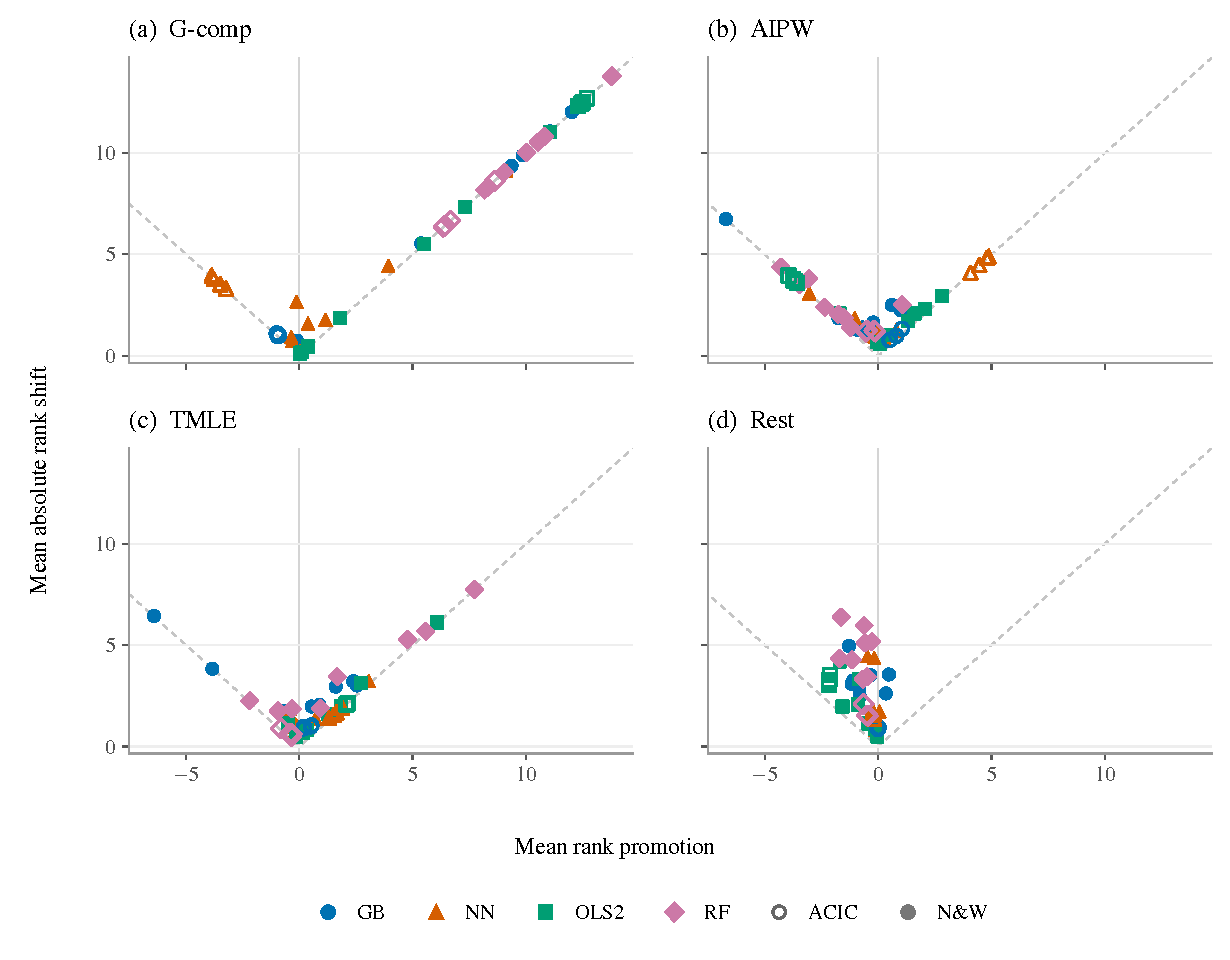
\includegraphics[width=0.75\textwidth]{figures/promotion_shift/promotion_shift.pdf}
\caption{Mean rank promotion and mean absolute rank shift for the associated G-comp, aligned AIPW, aligned TMLE, and non-aligned estimators (Rest; OLS1 is considered aligned with OLS2). Each point summarizes 100 reference datasets for one simulator and setting: open markers denote the four ACIC error structures; filled markers denote the eight N\&W DGP--sample-size settings. Colors and marker shapes identify simulators. Rest averages over non-aligned estimators; because promotions sum to zero, net aligned promotion implies net Rest demotion. Positive promotion indicates a higher rank under the simulator. The dashed boundary is $y=|x|$; points above it indicate rank movement in both directions across reference datasets (and, for Rest, estimators).}
\label{fig:promotion-shift}
\end{figure*}

\subsection{Ranking fidelity}

The fitted simulators can attain high ranking fidelity, but no single simulator performs best across all generators.

Table~\ref{tab:rank-aggregation} shows that, for ACIC, GB gives the highest mean rank correlation in each of the four error settings (0.942--0.946). NN (0.782--0.848) and RF (0.684--0.805) also attain relatively high correlations, although their ordering differs across error structures. RF has similar ranking fidelity under iid, group-correlated, and heteroskedastic errors (0.793--0.805), but its mean rank correlation falls to 0.684 under non-additive errors. GB remains stable, while NN has its highest mean rank correlation in the non-additive setting (0.848). OLS2 and WGAN have low ranking fidelity throughout (0.092--0.155 and 0.042--0.082, respectively). Overall, error structure appears to have a limited effect on ranking fidelity, with the clearest exception being RF under non-additive errors. Averaging the five simulator-specific rankings gives mean rank correlations of 0.899--0.919, below GB in every setting but above the other individual simulators. The aggregate mean rank correlation is lowest under non-additive errors.

The WGAN's low ranking fidelity in ACIC occurred despite diagnostic comparisons (not shown) similar to those presented by \authorcite{atheyUsingWassersteinGenerative2024}, in which the generated outcome distributions appeared reasonably similar to the observed ones. These checks therefore did not establish ranking fidelity.

The N\&W designs show stronger variation across settings and sample sizes (Table~\ref{tab:rank-aggregation}). GB has the highest mean rank correlation in A at both sample sizes (0.504 and 0.367), while OLS2 and NN perform best in B and C: OLS2 reaches 0.978 and 0.957 in C, and NN leads in B at \(n=4302\) (0.899). NN also leads in D, improving from 0.840 to 0.900 as the sample size increases. Larger samples do not uniformly improve ranking fidelity, however: in C, GB's mean rank correlation falls from 0.328 to -0.119 and RF's from -0.112 to -0.634. Rank aggregation gives mean rank correlations of 0.127--0.807 and remains below the best individual simulator in each setting. In C at \(n=4302\), for example, the aggregate mean rank correlation is 0.494 compared with 0.957 for OLS2. Averaged over all eight settings, NN has the highest mean rank correlation (0.717), followed by OLS2 (0.691), WGAN (0.458), GB (0.354), and RF (-0.055) (Table~\ref{tab:results_rho_all}).

\subsection{Model alignment}

Figure~\ref{fig:promotion-shift} shows that alignment affects estimator classes differently. G-comp exhibits the strongest upward rank promotion, whereas TMLE shows smaller and more variable promotion. AIPW promotions are generally centered near zero, with movement in both directions rather than a systematic upward shift. NN in ACIC is an exception, with aligned AIPW promoted by approximately four to five positions. Small mean promotion can also conceal movement in both directions, as indicated by points above the dashed boundary. Thus, sharing the simulator's outcome learner does not uniformly benefit all three estimator classes.

The largest G-comp promotions occur for OLS2 in ACIC, GB in N\&W, and RF in both design families. Table~\ref{tab:rank-aggregation} supports the importance of these aligned estimators for ranking disagreement: excluding them raises OLS2's ACIC rank correlations from 0.092--0.155 to 0.614--0.743 and RF's from 0.684--0.805 to 0.803--0.883. For GB in N\&W C at \(n=1000\), the correlation increases from 0.328 to 0.560. RF also improves after exclusion in every N\&W setting, although its correlation remains negative in several settings, including C at \(n=4302\) (-0.634 to -0.528). Alignment therefore explains part, but not all, of the ranking disagreement. These pronounced G-comp promotions coincide with poor target-benchmark performance of the associated G-comp estimators (Appendix Table~\ref{tab:results_mse_all}). In contrast, GB in ACIC shows little rank movement, and exclusion barely changes its correlations (0.942--0.946 versus 0.943--0.951). However, estimators already near the top of the target ranking have little room for promotion; an estimator ranked first can only remain first or be demoted. Small rank movements therefore do not rule out an accuracy gain under an aligned simulator. Still, comparing MSEs in Appendix Table~\ref{tab:results_mse_all} suggests that this is not the case for GB in ACIC.

Excluding aligned votes also changes rank aggregation (Table~\ref{tab:rank-aggregation}). In ACIC, correlations increase from 0.899--0.919 to 0.928--0.934. The N\&W results are mixed: exclusion improves aggregation in some settings, but lowers it in C at \(n=4302\) and D at \(n=1000\).

\subsection{Estimand fidelity and ranking fidelity}

Table~\ref{tab:rank-aggregation} reports mean absolute estimand differences alongside rank correlations; smaller differences indicate higher \emph{estimand fidelity}. Across the settings studied, high ranking fidelity is generally accompanied by high estimand fidelity. GB has the smallest mean absolute estimand difference in every ACIC setting (0.085--0.116), while OLS2 combines the smallest differences (0.029--0.056) with high ranking fidelity in N\&W B and C.

In some settings, however, high estimand fidelity is not accompanied by high ranking fidelity. Table~\ref{tab:rank-aggregation} shows that simulators can have similar mean absolute estimand differences but substantially different rank correlations. In N\&W B at \(n=4302\), GB has an estimand difference of 0.039, close to those of OLS2 (0.030) and NN (0.033), but a much lower mean rank correlation (0.316 versus 0.854 and 0.899). In D at the same sample size, GB and NN both have differences of approximately 0.040, yet mean rank correlations of 0.455 and 0.900. Excluding aligned estimators does not remove these contrasts: GB reaches only 0.512 in B and 0.605 in D, compared with NN's 0.906 and 0.911. The limitation is also evident for RF in A and D at \(n=4302\): relatively small differences (0.087 and 0.044) accompany mean rank correlations of -0.344 and 0.324, which remain -0.230 and 0.477 after exclusion.

\subsection{Estimator-selection regret}
\begin{table*}[!t]
\centering
\caption{Mean relative MSE regret (\%) across the 100 reference datasets in each setting. Within each dataset, regret is the percentage excess target-benchmark MSE over the smallest target MSE among all 15 estimators; these percentages are then averaged over the 100 reference datasets. So 0 means matching the target-best MSE, and 100 means twice that MSE. G-comp uses the associated G-computation estimator directly. All and Excl. use the estimator minimizing simulator MSE among all estimators or among non-aligned estimators, respectively. Bold marks the lowest value within each simulator--setting triplet, including ties. WGAN is omitted because it has no associated G-comp in the candidate set.}
\label{tab:gcomp-selection}
{
\tablebox{%
\begin{tabular}{l*{12}{r}}
\toprule
Generator & \multicolumn{3}{c}{GB} & \multicolumn{3}{c}{NN} & \multicolumn{3}{c}{OLS2} & \multicolumn{3}{c}{RF} \\
\cmidrule(lr){2-4}\cmidrule(lr){5-7}\cmidrule(lr){8-10}\cmidrule(lr){11-13}
 & G-comp & All & Excl. & G-comp & All & Excl. & G-comp & All & Excl. & G-comp & All & Excl. \\
\midrule
ACIC IID & \textbf{1.6} & 17.6 & 31.1 & 202.1 & 148.0 & \textbf{63.3} & 6647.4 & 6678.3 & \textbf{187.2} & 381.9 & 178.2 & \textbf{62.3} \\
ACIC Non-additive & \textbf{0.0} & 27.6 & 46.7 & 224.9 & 135.9 & \textbf{57.3} & 6944.1 & 7001.6 & \textbf{203.4} & 629.0 & 550.5 & \textbf{250.6} \\
ACIC Group-correlated & \textbf{0.9} & 18.5 & 30.6 & 97.9 & 153.9 & \textbf{81.1} & 7931.3 & 7962.7 & \textbf{93.3} & 446.3 & 198.4 & \textbf{71.3} \\
ACIC Heteroskedastic & \textbf{1.1} & 20.8 & 30.7 & 162.9 & 149.2 & \textbf{62.8} & 7013.1 & 7023.5 & \textbf{155.2} & 382.9 & 167.1 & \textbf{64.2} \\
\addlinespace[\tablepanelgap]
N\&W A, $n=1000$ & \textbf{1.3} & 26.8 & 44.7 & 216.9 & 168.2 & \textbf{156.0} & 47.2 & 45.8 & \textbf{3.4} & 175.7 & \textbf{131.9} & \textbf{131.9} \\
N\&W A, $n=4302$ & 70.9 & 60.8 & \textbf{28.9} & 508.2 & \textbf{137.9} & 138.0 & 351.2 & 351.2 & \textbf{69.9} & 421.8 & 325.2 & \textbf{312.9} \\
N\&W B, $n=1000$ & 115.5 & 79.3 & \textbf{28.4} & 9.4 & \textbf{3.6} & 4.1 & \textbf{2.6} & 2.9 & 10.7 & 1720.1 & 250.2 & \textbf{113.9} \\
N\&W B, $n=4302$ & 117.7 & 74.2 & \textbf{18.1} & 17.4 & \textbf{1.9} & 2.0 & \textbf{3.5} & \textbf{3.5} & 4.3 & 1698.6 & 160.5 & \textbf{117.5} \\
N\&W C, $n=1000$ & 779.1 & 727.8 & \textbf{227.5} & 47.3 & 15.6 & \textbf{8.2} & 0.6 & \textbf{0.4} & 43.6 & 6792.2 & 5590.6 & \textbf{779.1} \\
N\&W C, $n=4302$ & 812.5 & 649.9 & \textbf{460.3} & 39.9 & 23.1 & \textbf{15.3} & \textbf{0.1} & \textbf{0.1} & 33.5 & 12797.6 & 10333.9 & \textbf{1054.7} \\
N\&W D, $n=1000$ & \textbf{69.1} & 87.8 & 95.7 & \textbf{3.7} & 16.9 & 27.5 & 53.7 & 53.7 & \textbf{15.4} & 99.6 & 99.8 & \textbf{81.3} \\
N\&W D, $n=4302$ & 65.2 & 50.7 & \textbf{45.8} & 15.7 & \textbf{3.1} & 5.0 & 189.8 & 189.8 & \textbf{1.5} & 116.4 & 65.2 & \textbf{60.6} \\
% BEGIN WIN COUNTS
\midrule
Winner count & 6/12 & 0/12 & 6/12 & 1/12 & 4/12 & 7/12 & 1/12 & 3/12 & 8/12 & 0/12 & 1/12 & 12/12 \\
% END WIN COUNTS
\bottomrule
\end{tabular}%
}
}
\end{table*}


Table~\ref{tab:gcomp-selection} reports the mean relative MSE regret defined in Equation~\eqref{eq:relative-mse-regret}. It shows that simulator-based selection can be valuable even when ranking fidelity is poor, particularly after excluding aligned estimators. For example, under the OLS2 simulator in ACIC, direct G-comp and All-based selection both have mean relative MSE regret above 6600\%, whereas Excl.-based selection has the lowest regret of the three choices in every error setting (93.3--203.4\%). The same pattern appears for RF in N\&W C at \(n=4302\): regret falls from 12797.6\% for RF G-comp and 10333.9\% for All-based selection to 1054.7\% after exclusion. Although the remaining loss is substantial, selecting a non-aligned estimator is much preferable to directly using the poorly performing associated G-comp in these settings.

This benefit is not confined to the simulators with the lowest ranking fidelity. NN has comparatively high ranking fidelity in ACIC, yet Excl.-based selection gives the lowest mean regret in every error setting: 57.3--81.1\%, compared with 97.9--224.9\% for NN G-comp and 135.9--153.9\% for All-based selection. Thus, selection among non-aligned estimators using a reasonably faithful simulator can outperform direct G-comp based on its associated conditional-mean learner.

When the associated outcome model performs well, directly using G-comp can instead be preferable. GB G-comp has mean regret below 1.7\% throughout ACIC, compared with 17.6--27.6\% for All-based selection and 30.6--46.7\% after exclusion. OLS2 in N\&W B and C also favors direct G-comp or gives nearly indistinguishable results with All-based selection: at \(n=4302\), both choices have mean regret of 3.5\% in B and 0.1\% in C, while Excl.-based selection gives 4.3\% and 33.5\%, respectively. In these examples, the penalty for following the ranking rather than using a well-performing G-comp is much smaller than the loss from directly using the poor OLS2 or RF G-comp estimators instead of Excl.-based selection in the earlier comparisons.

\subsection{Outcome-distribution distances}

\begin{table*}[!t]
\centering
\caption{Mean within-reference-dataset Pearson correlations between outcome-distribution distance and Spearman ranking fidelity. The main panels compare all five simulators; sensitivity panels remove WGAN in ACIC and RF in N\&W, leaving four. Each correlation compares these simulators on the same reference dataset; coefficients are then averaged over the 100 reference datasets. All and Excl. aligned use ranking fidelity before and after excluding estimators aligned with each simulator, respectively. Negative values indicate that simulators with smaller distances tend to have higher ranking fidelity. Bold marks the most negative mean correlation within each setting and estimator panel, including ties based on unrounded means. Superscripts \(\dagger\), \(\ddagger\), and \(\S\) indicate negative correlations in at least 90\%, 95\%, and 99\% of reference datasets, respectively (do not confuse with significance levels). }
\label{tab:distance-ranking}
{
\makebox[\textwidth][c]{\begin{tabular}{lrrrr@{\hspace{\tablegroupsep}}rrrrrrrr@{\hspace{\tablegroupsep}}r}
\toprule
& \multicolumn{4}{c}{ACIC 2017} & \multicolumn{8}{c}{N\&W} & Winner count \\
\cmidrule(lr){2-5}\cmidrule(lr){6-13}\cmidrule(lr){14-14}
Distance & IID & \shortstack{Non-\\additive} & \shortstack{Group-\\correlated} & \shortstack{Hetero-\\skedastic} & \shortstack{A\\$n=1000$} & \shortstack{A\\$n=4302$} & \shortstack{B\\$n=1000$} & \shortstack{B\\$n=4302$} & \shortstack{C\\$n=1000$} & \shortstack{C\\$n=4302$} & \shortstack{D\\$n=1000$} & \shortstack{D\\$n=4302$} & Total \\
\midrule
\multicolumn{14}{l}{\textit{All estimators}} \\
$W_1$ & -0.049 & -0.402 & -0.119 & -0.071 & 0.029 & \textbf{-0.098} & \textbf{-0.159} & \textbf{-0.392} & \textbf{-0.261} & \textbf{-0.420} & \textbf{-0.344} & \textbf{-0.389} & 7/12 \\
KS & \textbf{-0.351} & \textbf{-0.539}\textsuperscript{\(\dagger\)} & \textbf{-0.422} & \textbf{-0.377} & 0.015 & 0.116 & -0.009 & -0.041 & -0.027 & -0.042 & -0.192 & -0.146 & 4/12 \\
Energy & -0.179 & -0.529 & -0.254 & -0.209 & \textbf{0.015} & -0.004 & -0.097 & -0.247 & -0.194 & -0.313 & -0.276 & -0.288 & 1/12 \\
\addlinespace[\tablepanelgap]
\multicolumn{14}{l}{\textit{Excl. aligned}} \\
$W_1$ & -0.329 & -0.569 & -0.413 & -0.365 & \textbf{-0.058} & \textbf{0.001} & \textbf{-0.186} & \textbf{-0.424}\textsuperscript{\(\dagger\)} & \textbf{-0.337} & \textbf{-0.452} & \textbf{-0.383} & \textbf{-0.539} & 8/12 \\
KS & \textbf{-0.662}\textsuperscript{\(\dagger\)} & \textbf{-0.706}\textsuperscript{\(\dagger\)} & \textbf{-0.736}\textsuperscript{\(\dagger\)} & \textbf{-0.706}\textsuperscript{\(\ddagger\)} & -0.025 & 0.071 & -0.078 & -0.110 & -0.142 & -0.085 & -0.221 & -0.265 & 4/12 \\
Energy & -0.482 & -0.680 & -0.566\textsuperscript{\(\dagger\)} & -0.527 & -0.046 & 0.034 & -0.142 & -0.300 & -0.287 & -0.351 & -0.316 & -0.451 & 0/12 \\
\addlinespace[\tablepanelgap]
\multicolumn{14}{l}{\textit{All estimators; WGAN / RF removed}} \\
$W_1$ & 0.386 & -0.254 & 0.376 & 0.384 & -0.051 & 0.366 & \textbf{-0.602}\textsuperscript{\(\ddagger\)} & \textbf{-0.488} & \textbf{-0.620}\textsuperscript{\(\dagger\)} & \textbf{-0.475} & \textbf{-0.453} & \textbf{-0.329} & 6/12 \\
KS & \textbf{0.334} & -0.457\textsuperscript{\(\ddagger\)} & \textbf{0.315} & \textbf{0.322} & \textbf{-0.174} & \textbf{0.253} & -0.455 & -0.220 & -0.392 & -0.136 & -0.303 & -0.192 & 5/12 \\
Energy & 0.379 & \textbf{-0.585}\textsuperscript{\(\ddagger\)} & 0.366 & 0.372 & -0.115 & 0.325 & -0.540\textsuperscript{\(\dagger\)} & -0.367 & -0.568\textsuperscript{\(\dagger\)} & -0.358 & -0.390 & -0.269 & 1/12 \\
\addlinespace[\tablepanelgap]
\multicolumn{14}{l}{\textit{Excl. aligned; WGAN / RF removed}} \\
$W_1$ & 0.342 & -0.302 & 0.281 & 0.331 & -0.153 & 0.395 & \textbf{-0.679}\textsuperscript{\(\ddagger\)} & \textbf{-0.618}\textsuperscript{\(\ddagger\)} & \textbf{-0.717}\textsuperscript{\(\ddagger\)} & \textbf{-0.530}\textsuperscript{\(\dagger\)} & \textbf{-0.478} & \textbf{-0.522} & 6/12 \\
KS & \textbf{0.256} & -0.494\textsuperscript{\(\dagger\)} & \textbf{0.177} & \textbf{0.230} & \textbf{-0.198} & \textbf{0.142} & -0.600\textsuperscript{\(\dagger\)} & -0.407 & -0.528 & -0.204 & -0.319 & -0.316 & 5/12 \\
Energy & 0.323 & \textbf{-0.585}\textsuperscript{\(\ddagger\)} & 0.254 & 0.305 & -0.177 & 0.291 & -0.649\textsuperscript{\(\dagger\)} & -0.529\textsuperscript{\(\dagger\)} & -0.684\textsuperscript{\(\ddagger\)} & -0.419 & -0.414 & -0.457 & 1/12 \\
\bottomrule
\end{tabular}}
}
\end{table*}


For each reference dataset, we compute the Pearson correlation across the five simulators between outcome-distribution distance and ranking fidelity, then average these correlations over the 100 reference datasets in each setting. Negative correlations indicate that simulators whose generated outcomes are closer to the observed outcomes tend to give more faithful rankings on the same reference dataset.

With all five simulators, Table~\ref{tab:distance-ranking} shows predominantly negative mean correlations, generally stronger after excluding aligned estimators. KS has the most negative mean correlation in every ACIC setting, both before and after exclusion. In N\&W, Wasserstein distance has the most negative mean correlation in seven of eight settings before exclusion and all eight afterward. The N\&W associations are clearest in B--D, while those in A are near zero or mixed in sign.

These averages conceal substantial variation across reference datasets. In the five-simulator analysis, only one comparison using all estimators and six after excluding aligned estimators have negative correlations in at least 90\% of reference datasets. The highest proportion is 95\%, attained by KS in the ACIC heteroskedastic setting after exclusion.

Furthermore, each correlation uses only five simulators and is therefore sensitive to individual simulators with extreme distances or ranking fidelity. Table~\ref{tab:distance-ranking} also reports sensitivity checks removing the simulator with the lowest ranking fidelity in each design family. Removing WGAN in ACIC reversed the mean correlations from negative to positive for all three distances in every setting except non-additive errors, both before and after excluding aligned estimators. Removing RF in N\&W, by contrast, generally strengthened the negative associations in B--D: all three distances retained negative mean correlations at both sample sizes, before and after exclusion. In A, the correlations remained inconsistent, becoming negative at \(n=1000\) and positive at \(n=4302\) for all three distances and both estimator sets.

% !TeX root = Master.tex
\section{Discussion}
\label{sec:discussion}

This paper formalizes the objectives and assumptions of empirical Monte Carlo benchmarking and examines whether fitted outcome simulators preserve estimator rankings. The results suggest that ranking fidelity depends on the simulator, the candidate estimators, and the underlying DGP. The variation across simulators is consistent with the sensitivity to simulation models reported by \authorcite{gentzelCaseEvaluatingCausal} and \authorcite{amaranathImprovingGenerativeMethods}. Variation across N\&W designs was greater than across ACIC error structures, pointing to the importance of conditional outcome structure and treatment confounding; RF under non-additive errors was the clearest error-structure exception. Larger reference samples sometimes substantially changed fidelity, but did not consistently improve it. Aggregating rankings may offer a robustness check under model uncertainty, although it never outperformed the best individual simulator and was not uniformly reliable.

Model alignment is a central concern because a simulator can favor estimators sharing its outcome-model specification, particularly when that model poorly approximates the target outcome structure. G-computation showed the strongest promotions, TMLE was less affected, and AIPW generally showed little promotion or slight demotion. Excluding aligned estimators substantially improved ranking fidelity in some settings, but poor fidelity sometimes persisted and exclusion did not always help. Alignment therefore explains part of the disagreement between benchmarks, rather than all simulator failures. Its model-dependence agrees with \authorcite{schulerSynthValidationSelectingBest2017}, who found alignment effects for linear regression and unconstrained gradient boosting, and \authorcite{karimPlasmodeBenchmarkCan2026}, who demonstrated alignment bias for a parametric outcome model. OLS2 showed the largest exclusion-related improvements in ACIC, while the effects for flexible learners were more varied.

Estimand fidelity and ranking fidelity were generally closely related. Nevertheless, similar mean absolute estimand differences sometimes accompanied substantially different rankings, even after excluding aligned estimators. These results provide some evidence that matching the reference effect is not enough to ensure ranking fidelity, illustrating the distinction between estimand transfer and ranking transfer made by \authorcite{karimPlasmodeBenchmarkCan2026}.

The regret comparisons answer the question of whether conducting an EMCS for estimator selection adds value over using the associated G-computation estimator. In line with \authorcite{advaniMostlyHarmlessSimulations2019}, misspecified models can mislead estimator comparisons. Our regret results also show that such simulators may still be useful for selection when aligned estimators are excluded, potentially reducing regret under model uncertainty. When an outcome model is well supported, direct G-computation may be preferable, while selection from its full induced ranking generally incurs a comparatively small penalty. The value of an EMCS thus depends on prior confidence in the model and which estimators remain eligible for selection.

The low ranking fidelity of WGAN in ACIC despite reasonable distributional diagnostics (not shown) suggests that checks similar to those proposed by \authorcite{atheyUsingWassersteinGenerative2024} are insufficient on their own to validate a benchmark for estimator selection. The distance associations and sensitivity checks suggest that outcome similarity may identify pronounced simulator failures, but can be less useful for distinguishing among the remaining alternatives. The greater robustness of the N\&W B--D associations shows that this limitation is setting-dependent.

Consequently, no simulator should be expected to provide universally reliable rankings across all empirical settings. A practical approach could be to fit several simulation models, use outcome distances as exploratory diagnostics alongside prior knowledge and other checks to assess confidence in each, and compare the resulting rankings after excluding aligned estimators. An aggregate ranking can provide a robustness check or a default when there is little basis for preferring one simulator, although our results do not establish it as superior to individual models. When an outcome model is already well supported, using it directly for G-comp or selecting an estimator from its full induced ranking, without excluding aligned estimators, may be preferable.

Finally, several limitations should be noted. Our simulation design holds covariates and treatment fixed within each benchmark and simulates only outcomes. The findings therefore only partially extend to EMCS that also model treatment assignment or the covariate distribution. Further work is needed to assess how approximation of these additional components, such as the propensity score, can distort estimator comparisons and interact with outcome-model approximation and model alignment. The evidence comes from two families of designs (ACIC 2017 and the N\&W designs with six covariates), with simulators and outcome learners fitted with fixed hyperparameter settings to facilitate comparisons and reduce variation from tuning. It remains unclear how well the findings generalize to other designs, or how much tuning would change the results or improve the performance of models such as RF. The WGAN results concern a single specification; alternative architectures and training procedures may yield different findings. Comparing alternative models and architectures could help establish whether the failures observed here persist and clarify how model alignment arises, including within model families.

Another limitation of our evaluation is our reliance mainly on averages across reference datasets, although we performed a sensitivity check using medians and obtained generally similar findings. The biggest differences concerned regret magnitudes, which sometimes changed substantially, although the mean-optimal selection rule remained optimal under the median in all cases. Our evaluation relies mainly on Spearman rank correlation and estimator-selection regret; although checks using Kendall's \(\tau\) gave largely consistent comparisons, other measures could reveal aspects of benchmark performance that these summaries miss. We do not show these robustness checks. Estimator comparison focused on MSE only. A particularly interesting direction for future work could be to extend evaluations to the accuracy of estimated standard errors and confidence-interval coverage. This would also assess whether simulators reproduce inferential performance, which preservation of MSE rankings alone does not guarantee.

\section*{Code and Data Availability}
\label{sec:code-data-availability}
The simulation code and numerical results needed to reproduce the tables and figures are available at \url{https://github.com/carlosrameal/emcs-rank-preservation}.
\bibliographystyle{paper-references}
\bibliography{references}
\clearpage
\onecolumn
% Geometry changes in the appendix must retain its single-column layout.
\let\preprintnewgeometry\newgeometry
\renewcommand{\newgeometry}[1]{\preprintnewgeometry{#1}\onecolumn}
\appendix
\setcounter{figure}{0}
\setcounter{table}{0}
\renewcommand{\thefigure}{A\arabic{figure}}
\renewcommand{\thetable}{A\arabic{table}}
% !TeX root = Master.tex
\ifdefined\neutralpreprint
\newgeometry{top=10mm,bottom=10mm,left=12mm,right=12mm}
\begin{landscape}
\fi
\section{Detailed results}
\label{app:complete-results}

This appendix complements Section~\ref{sec:results} with detailed MSE, rank-correlation, and rank-movement results, together with distributions of rank correlations, for all four ACIC error structures and all four N\&W designs at both sample sizes.

\ifdefined\neutralpreprint\else
\newgeometry{top=10mm,bottom=10mm,left=12mm,right=12mm}
\begin{landscape}
\fi
\begingroup
\renewcommand{\papertablestyle}{\fontsize{7.5}{10}\selectfont\setlength{\tabcolsep}{0.5pt}\renewcommand{\arraystretch}{1}}
\begin{longtable}{*{7}{c}@{\hspace{6pt}}*{7}{c}@{\hspace{6pt}}*{7}{c}@{\hspace{6pt}}*{7}{c}}
\caption{Average Monte Carlo MSE by estimator and benchmark, averaged over 100 reference datasets per setting. Each setting has its own estimator order, from lowest to highest target-benchmark MSE.}\label{tab:results_mse_all} \\
\toprule
\makebox[54pt][c]{Estimator} & \makebox[19pt][c]{Target} & \makebox[19pt][c]{GB} & \makebox[19pt][c]{NN} & \makebox[19pt][c]{OLS2} & \makebox[19pt][c]{RF} & \makebox[19pt][c]{WGAN} & \makebox[54pt][c]{Estimator} & \makebox[19pt][c]{Target} & \makebox[19pt][c]{GB} & \makebox[19pt][c]{NN} & \makebox[19pt][c]{OLS2} & \makebox[19pt][c]{RF} & \makebox[19pt][c]{WGAN} & \makebox[54pt][c]{Estimator} & \makebox[19pt][c]{Target} & \makebox[19pt][c]{GB} & \makebox[19pt][c]{NN} & \makebox[19pt][c]{OLS2} & \makebox[19pt][c]{RF} & \makebox[19pt][c]{WGAN} & \makebox[54pt][c]{Estimator} & \makebox[19pt][c]{Target} & \makebox[19pt][c]{GB} & \makebox[19pt][c]{NN} & \makebox[19pt][c]{OLS2} & \makebox[19pt][c]{RF} & \makebox[19pt][c]{WGAN} \\
\midrule
\endfirsthead
\caption[]{Average Monte Carlo MSE by estimator and benchmark, averaged over 100 reference datasets per setting (continued).} \\
\toprule
\makebox[54pt][c]{Estimator} & \makebox[19pt][c]{Target} & \makebox[19pt][c]{GB} & \makebox[19pt][c]{NN} & \makebox[19pt][c]{OLS2} & \makebox[19pt][c]{RF} & \makebox[19pt][c]{WGAN} & \makebox[54pt][c]{Estimator} & \makebox[19pt][c]{Target} & \makebox[19pt][c]{GB} & \makebox[19pt][c]{NN} & \makebox[19pt][c]{OLS2} & \makebox[19pt][c]{RF} & \makebox[19pt][c]{WGAN} & \makebox[54pt][c]{Estimator} & \makebox[19pt][c]{Target} & \makebox[19pt][c]{GB} & \makebox[19pt][c]{NN} & \makebox[19pt][c]{OLS2} & \makebox[19pt][c]{RF} & \makebox[19pt][c]{WGAN} & \makebox[54pt][c]{Estimator} & \makebox[19pt][c]{Target} & \makebox[19pt][c]{GB} & \makebox[19pt][c]{NN} & \makebox[19pt][c]{OLS2} & \makebox[19pt][c]{RF} & \makebox[19pt][c]{WGAN} \\
\midrule
\endhead
\midrule
\multicolumn{28}{r}{Continued on next page} \\
\endfoot
\bottomrule
\endlastfoot
\multicolumn{7}{c}{\textit{ACIC IID}} & \multicolumn{7}{c}{\textit{ACIC Non-additive}} & \multicolumn{7}{c}{\textit{ACIC Group-correlated}} & \multicolumn{7}{c}{\textit{ACIC Heteroskedastic}} \\*
\cmidrule(lr){1-7}\cmidrule(lr){8-14}\cmidrule(lr){15-21}\cmidrule(lr){22-28}
\makebox[54pt][c]{GB G-comp} & \makebox[19pt][c]{0.013} & \makebox[19pt][c]{0.020} & \makebox[19pt][c]{0.041} & \makebox[19pt][c]{0.014} & \makebox[19pt][c]{0.025} & \makebox[19pt][c]{1.879} & \makebox[54pt][c]{GB G-comp} & \makebox[19pt][c]{0.021} & \makebox[19pt][c]{0.035} & \makebox[19pt][c]{0.064} & \makebox[19pt][c]{0.026} & \makebox[19pt][c]{0.065} & \makebox[19pt][c]{3.521} & \makebox[54pt][c]{GB G-comp} & \makebox[19pt][c]{0.011} & \makebox[19pt][c]{0.017} & \makebox[19pt][c]{0.041} & \makebox[19pt][c]{0.012} & \makebox[19pt][c]{0.021} & \makebox[19pt][c]{1.804} & \makebox[54pt][c]{GB G-comp} & \makebox[19pt][c]{0.012} & \makebox[19pt][c]{0.020} & \makebox[19pt][c]{0.042} & \makebox[19pt][c]{0.014} & \makebox[19pt][c]{0.023} & \makebox[19pt][c]{1.771} \\*
\makebox[54pt][c]{BCF G-comp} & \makebox[19pt][c]{0.015} & \makebox[19pt][c]{0.019} & \makebox[19pt][c]{0.034} & \makebox[19pt][c]{0.018} & \makebox[19pt][c]{0.040} & \makebox[19pt][c]{2.222} & \makebox[54pt][c]{BCF G-comp} & \makebox[19pt][c]{0.029} & \makebox[19pt][c]{0.033} & \makebox[19pt][c]{0.054} & \makebox[19pt][c]{0.034} & \makebox[19pt][c]{0.105} & \makebox[19pt][c]{4.100} & \makebox[54pt][c]{BCF G-comp} & \makebox[19pt][c]{0.014} & \makebox[19pt][c]{0.016} & \makebox[19pt][c]{0.029} & \makebox[19pt][c]{0.016} & \makebox[19pt][c]{0.041} & \makebox[19pt][c]{2.106} & \makebox[54pt][c]{BCF G-comp} & \makebox[19pt][c]{0.015} & \makebox[19pt][c]{0.018} & \makebox[19pt][c]{0.033} & \makebox[19pt][c]{0.018} & \makebox[19pt][c]{0.039} & \makebox[19pt][c]{2.132} \\*
\makebox[54pt][c]{GB--OLS2 AIPW} & \makebox[19pt][c]{0.022} & \makebox[19pt][c]{0.030} & \makebox[19pt][c]{0.043} & \makebox[19pt][c]{0.030} & \makebox[19pt][c]{0.035} & \makebox[19pt][c]{1.623} & \makebox[54pt][c]{GB--OLS2 AIPW} & \makebox[19pt][c]{0.036} & \makebox[19pt][c]{0.051} & \makebox[19pt][c]{0.070} & \makebox[19pt][c]{0.054} & \makebox[19pt][c]{0.079} & \makebox[19pt][c]{3.096} & \makebox[54pt][c]{GB--OLS2 AIPW} & \makebox[19pt][c]{0.019} & \makebox[19pt][c]{0.025} & \makebox[19pt][c]{0.042} & \makebox[19pt][c]{0.027} & \makebox[19pt][c]{0.030} & \makebox[19pt][c]{1.638} & \makebox[54pt][c]{GB--OLS2 AIPW} & \makebox[19pt][c]{0.021} & \makebox[19pt][c]{0.028} & \makebox[19pt][c]{0.043} & \makebox[19pt][c]{0.029} & \makebox[19pt][c]{0.033} & \makebox[19pt][c]{1.611} \\*
\makebox[54pt][c]{GB--GB AIPW} & \makebox[19pt][c]{0.027} & \makebox[19pt][c]{0.031} & \makebox[19pt][c]{0.033} & \makebox[19pt][c]{0.037} & \makebox[19pt][c]{0.055} & \makebox[19pt][c]{1.161} & \makebox[54pt][c]{GB--GB AIPW} & \makebox[19pt][c]{0.044} & \makebox[19pt][c]{0.052} & \makebox[19pt][c]{0.056} & \makebox[19pt][c]{0.067} & \makebox[19pt][c]{0.121} & \makebox[19pt][c]{2.200} & \makebox[54pt][c]{NN G-comp} & \makebox[19pt][c]{0.022} & \makebox[19pt][c]{0.054} & \makebox[19pt][c]{0.078} & \makebox[19pt][c]{0.010} & \makebox[19pt][c]{0.046} & \makebox[19pt][c]{1.400} & \makebox[54pt][c]{GB--GB AIPW} & \makebox[19pt][c]{0.025} & \makebox[19pt][c]{0.029} & \makebox[19pt][c]{0.031} & \makebox[19pt][c]{0.036} & \makebox[19pt][c]{0.052} & \makebox[19pt][c]{1.135} \\*
\makebox[54pt][c]{GB--RF AIPW} & \makebox[19pt][c]{0.027} & \makebox[19pt][c]{0.034} & \makebox[19pt][c]{0.043} & \makebox[19pt][c]{0.047} & \makebox[19pt][c]{0.044} & \makebox[19pt][c]{1.240} & \makebox[54pt][c]{GB--RF AIPW} & \makebox[19pt][c]{0.045} & \makebox[19pt][c]{0.059} & \makebox[19pt][c]{0.071} & \makebox[19pt][c]{0.086} & \makebox[19pt][c]{0.084} & \makebox[19pt][c]{2.218} & \makebox[54pt][c]{GB--GB AIPW} & \makebox[19pt][c]{0.022} & \makebox[19pt][c]{0.026} & \makebox[19pt][c]{0.029} & \makebox[19pt][c]{0.033} & \makebox[19pt][c]{0.049} & \makebox[19pt][c]{1.099} & \makebox[54pt][c]{GB--RF AIPW} & \makebox[19pt][c]{0.026} & \makebox[19pt][c]{0.033} & \makebox[19pt][c]{0.042} & \makebox[19pt][c]{0.047} & \makebox[19pt][c]{0.042} & \makebox[19pt][c]{1.199} \\*
\makebox[54pt][c]{NN G-comp} & \makebox[19pt][c]{0.039} & \makebox[19pt][c]{0.095} & \makebox[19pt][c]{0.112} & \makebox[19pt][c]{0.012} & \makebox[19pt][c]{0.081} & \makebox[19pt][c]{1.474} & \makebox[54pt][c]{GB--NN AIPW} & \makebox[19pt][c]{0.069} & \makebox[19pt][c]{0.065} & \makebox[19pt][c]{0.048} & \makebox[19pt][c]{0.056} & \makebox[19pt][c]{0.153} & \makebox[19pt][c]{1.834} & \makebox[54pt][c]{GB--RF AIPW} & \makebox[19pt][c]{0.022} & \makebox[19pt][c]{0.029} & \makebox[19pt][c]{0.039} & \makebox[19pt][c]{0.043} & \makebox[19pt][c]{0.038} & \makebox[19pt][c]{1.188} & \makebox[54pt][c]{NN G-comp} & \makebox[19pt][c]{0.032} & \makebox[19pt][c]{0.081} & \makebox[19pt][c]{0.102} & \makebox[19pt][c]{0.011} & \makebox[19pt][c]{0.070} & \makebox[19pt][c]{1.382} \\*
\makebox[54pt][c]{GB--NN AIPW} & \makebox[19pt][c]{0.042} & \makebox[19pt][c]{0.040} & \makebox[19pt][c]{0.027} & \makebox[19pt][c]{0.031} & \makebox[19pt][c]{0.071} & \makebox[19pt][c]{0.926} & \makebox[54pt][c]{NN G-comp} & \makebox[19pt][c]{0.069} & \makebox[19pt][c]{0.175} & \makebox[19pt][c]{0.200} & \makebox[19pt][c]{0.023} & \makebox[19pt][c]{0.119} & \makebox[19pt][c]{2.905} & \makebox[54pt][c]{GB--NN AIPW} & \makebox[19pt][c]{0.040} & \makebox[19pt][c]{0.038} & \makebox[19pt][c]{0.022} & \makebox[19pt][c]{0.028} & \makebox[19pt][c]{0.072} & \makebox[19pt][c]{0.874} & \makebox[54pt][c]{GB--NN AIPW} & \makebox[19pt][c]{0.042} & \makebox[19pt][c]{0.038} & \makebox[19pt][c]{0.025} & \makebox[19pt][c]{0.031} & \makebox[19pt][c]{0.071} & \makebox[19pt][c]{0.898} \\*
\makebox[54pt][c]{RF G-comp} & \makebox[19pt][c]{0.063} & \makebox[19pt][c]{0.076} & \makebox[19pt][c]{0.105} & \makebox[19pt][c]{0.021} & \makebox[19pt][c]{0.024} & \makebox[19pt][c]{2.367} & \makebox[54pt][c]{GB--GB TMLE} & \makebox[19pt][c]{0.109} & \makebox[19pt][c]{0.132} & \makebox[19pt][c]{0.102} & \makebox[19pt][c]{0.149} & \makebox[19pt][c]{0.222} & \makebox[19pt][c]{1.292} & \makebox[54pt][c]{GB--GB TMLE} & \makebox[19pt][c]{0.057} & \makebox[19pt][c]{0.069} & \makebox[19pt][c]{0.046} & \makebox[19pt][c]{0.074} & \makebox[19pt][c]{0.101} & \makebox[19pt][c]{0.633} & \makebox[54pt][c]{RF G-comp} & \makebox[19pt][c]{0.059} & \makebox[19pt][c]{0.073} & \makebox[19pt][c]{0.107} & \makebox[19pt][c]{0.021} & \makebox[19pt][c]{0.023} & \makebox[19pt][c]{2.245} \\*
\makebox[54pt][c]{GB--GB TMLE} & \makebox[19pt][c]{0.067} & \makebox[19pt][c]{0.080} & \makebox[19pt][c]{0.056} & \makebox[19pt][c]{0.083} & \makebox[19pt][c]{0.113} & \makebox[19pt][c]{0.699} & \makebox[54pt][c]{RF G-comp} & \makebox[19pt][c]{0.155} & \makebox[19pt][c]{0.146} & \makebox[19pt][c]{0.166} & \makebox[19pt][c]{0.039} & \makebox[19pt][c]{0.033} & \makebox[19pt][c]{4.147} & \makebox[54pt][c]{RF G-comp} & \makebox[19pt][c]{0.060} & \makebox[19pt][c]{0.071} & \makebox[19pt][c]{0.109} & \makebox[19pt][c]{0.019} & \makebox[19pt][c]{0.021} & \makebox[19pt][c]{2.373} & \makebox[54pt][c]{GB--GB TMLE} & \makebox[19pt][c]{0.063} & \makebox[19pt][c]{0.074} & \makebox[19pt][c]{0.052} & \makebox[19pt][c]{0.081} & \makebox[19pt][c]{0.107} & \makebox[19pt][c]{0.688} \\*
\makebox[54pt][c]{GB--RF TMLE} & \makebox[19pt][c]{0.097} & \makebox[19pt][c]{0.107} & \makebox[19pt][c]{0.070} & \makebox[19pt][c]{0.102} & \makebox[19pt][c]{0.148} & \makebox[19pt][c]{0.605} & \makebox[54pt][c]{GB--RF TMLE} & \makebox[19pt][c]{0.157} & \makebox[19pt][c]{0.176} & \makebox[19pt][c]{0.128} & \makebox[19pt][c]{0.183} & \makebox[19pt][c]{0.284} & \makebox[19pt][c]{1.069} & \makebox[54pt][c]{GB--RF TMLE} & \makebox[19pt][c]{0.086} & \makebox[19pt][c]{0.095} & \makebox[19pt][c]{0.059} & \makebox[19pt][c]{0.092} & \makebox[19pt][c]{0.132} & \makebox[19pt][c]{0.526} & \makebox[54pt][c]{GB--RF TMLE} & \makebox[19pt][c]{0.092} & \makebox[19pt][c]{0.100} & \makebox[19pt][c]{0.065} & \makebox[19pt][c]{0.101} & \makebox[19pt][c]{0.140} & \makebox[19pt][c]{0.583} \\*
\makebox[54pt][c]{GB IPW} & \makebox[19pt][c]{0.106} & \makebox[19pt][c]{0.117} & \makebox[19pt][c]{0.185} & \makebox[19pt][c]{0.122} & \makebox[19pt][c]{0.059} & \makebox[19pt][c]{2.274} & \makebox[54pt][c]{GB IPW} & \makebox[19pt][c]{0.184} & \makebox[19pt][c]{0.211} & \makebox[19pt][c]{0.320} & \makebox[19pt][c]{0.225} & \makebox[19pt][c]{0.078} & \makebox[19pt][c]{4.165} & \makebox[54pt][c]{GB IPW} & \makebox[19pt][c]{0.103} & \makebox[19pt][c]{0.111} & \makebox[19pt][c]{0.184} & \makebox[19pt][c]{0.119} & \makebox[19pt][c]{0.055} & \makebox[19pt][c]{2.219} & \makebox[54pt][c]{GB IPW} & \makebox[19pt][c]{0.105} & \makebox[19pt][c]{0.117} & \makebox[19pt][c]{0.185} & \makebox[19pt][c]{0.121} & \makebox[19pt][c]{0.059} & \makebox[19pt][c]{2.187} \\*
\makebox[54pt][c]{GB--NN TMLE} & \makebox[19pt][c]{0.193} & \makebox[19pt][c]{0.240} & \makebox[19pt][c]{0.121} & \makebox[19pt][c]{0.081} & \makebox[19pt][c]{0.398} & \makebox[19pt][c]{0.574} & \makebox[54pt][c]{GB--NN TMLE} & \makebox[19pt][c]{0.316} & \makebox[19pt][c]{0.403} & \makebox[19pt][c]{0.228} & \makebox[19pt][c]{0.146} & \makebox[19pt][c]{0.779} & \makebox[19pt][c]{1.103} & \makebox[54pt][c]{GB--NN TMLE} & \makebox[19pt][c]{0.152} & \makebox[19pt][c]{0.194} & \makebox[19pt][c]{0.096} & \makebox[19pt][c]{0.072} & \makebox[19pt][c]{0.325} & \makebox[19pt][c]{0.519} & \makebox[54pt][c]{GB--NN TMLE} & \makebox[19pt][c]{0.180} & \makebox[19pt][c]{0.220} & \makebox[19pt][c]{0.113} & \makebox[19pt][c]{0.080} & \makebox[19pt][c]{0.373} & \makebox[19pt][c]{0.558} \\*
\makebox[54pt][c]{GB--OLS2 TMLE} & \makebox[19pt][c]{0.712} & \makebox[19pt][c]{0.662} & \makebox[19pt][c]{0.365} & \makebox[19pt][c]{0.079} & \makebox[19pt][c]{0.812} & \makebox[19pt][c]{0.403} & \makebox[54pt][c]{GB--OLS2 TMLE} & \makebox[19pt][c]{1.252} & \makebox[19pt][c]{1.162} & \makebox[19pt][c]{0.652} & \makebox[19pt][c]{0.143} & \makebox[19pt][c]{1.543} & \makebox[19pt][c]{0.824} & \makebox[54pt][c]{GB--OLS2 TMLE} & \makebox[19pt][c]{0.701} & \makebox[19pt][c]{0.658} & \makebox[19pt][c]{0.390} & \makebox[19pt][c]{0.071} & \makebox[19pt][c]{0.802} & \makebox[19pt][c]{0.347} & \makebox[54pt][c]{GB--OLS2 TMLE} & \makebox[19pt][c]{0.709} & \makebox[19pt][c]{0.654} & \makebox[19pt][c]{0.373} & \makebox[19pt][c]{0.078} & \makebox[19pt][c]{0.808} & \makebox[19pt][c]{0.409} \\*
\makebox[54pt][c]{OLS2 G-comp} & \makebox[19pt][c]{0.869} & \makebox[19pt][c]{0.859} & \makebox[19pt][c]{0.777} & \makebox[19pt][c]{0.009} & \makebox[19pt][c]{0.590} & \makebox[19pt][c]{4.795} & \makebox[54pt][c]{OLS2 G-comp} & \makebox[19pt][c]{1.487} & \makebox[19pt][c]{1.498} & \makebox[19pt][c]{1.275} & \makebox[19pt][c]{0.017} & \makebox[19pt][c]{0.866} & \makebox[19pt][c]{8.432} & \makebox[54pt][c]{OLS2 G-comp} & \makebox[19pt][c]{0.867} & \makebox[19pt][c]{0.847} & \makebox[19pt][c]{0.842} & \makebox[19pt][c]{0.008} & \makebox[19pt][c]{0.590} & \makebox[19pt][c]{5.021} & \makebox[54pt][c]{OLS2 G-comp} & \makebox[19pt][c]{0.868} & \makebox[19pt][c]{0.864} & \makebox[19pt][c]{0.813} & \makebox[19pt][c]{0.009} & \makebox[19pt][c]{0.598} & \makebox[19pt][c]{4.614} \\*
\makebox[54pt][c]{OLS1} & \makebox[19pt][c]{0.887} & \makebox[19pt][c]{0.877} & \makebox[19pt][c]{0.795} & \makebox[19pt][c]{0.009} & \makebox[19pt][c]{0.604} & \makebox[19pt][c]{4.842} & \makebox[54pt][c]{OLS1} & \makebox[19pt][c]{1.541} & \makebox[19pt][c]{1.553} & \makebox[19pt][c]{1.327} & \makebox[19pt][c]{0.018} & \makebox[19pt][c]{0.906} & \makebox[19pt][c]{8.648} & \makebox[54pt][c]{OLS1} & \makebox[19pt][c]{0.885} & \makebox[19pt][c]{0.865} & \makebox[19pt][c]{0.861} & \makebox[19pt][c]{0.008} & \makebox[19pt][c]{0.604} & \makebox[19pt][c]{5.075} & \makebox[54pt][c]{OLS1} & \makebox[19pt][c]{0.887} & \makebox[19pt][c]{0.882} & \makebox[19pt][c]{0.831} & \makebox[19pt][c]{0.009} & \makebox[19pt][c]{0.611} & \makebox[19pt][c]{4.683} \\
\addlinespace[14pt]
\multicolumn{7}{c}{\textit{N\&W A, $n=1000$}} & \multicolumn{7}{c}{\textit{N\&W A, $n=4302$}} & \multicolumn{7}{c}{\textit{N\&W B, $n=1000$}} & \multicolumn{7}{c}{\textit{N\&W B, $n=4302$}} \\*
\cmidrule(lr){1-7}\cmidrule(lr){8-14}\cmidrule(lr){15-21}\cmidrule(lr){22-28}
\makebox[54pt][c]{GB G-comp} & \makebox[19pt][c]{0.010} & \makebox[19pt][c]{0.009} & \makebox[19pt][c]{0.008} & \makebox[19pt][c]{0.007} & \makebox[19pt][c]{0.011} & \makebox[19pt][c]{0.003} & \makebox[54pt][c]{GB--GB TMLE} & \makebox[19pt][c]{0.002} & \makebox[19pt][c]{0.003} & \makebox[19pt][c]{0.002} & \makebox[19pt][c]{0.002} & \makebox[19pt][c]{0.005} & \makebox[19pt][c]{0.001} & \makebox[54pt][c]{OLS2 G-comp} & \makebox[19pt][c]{0.004} & \makebox[19pt][c]{0.009} & \makebox[19pt][c]{0.005} & \makebox[19pt][c]{0.005} & \makebox[19pt][c]{0.026} & \makebox[19pt][c]{0.001} & \makebox[54pt][c]{OLS2 G-comp} & \makebox[19pt][c]{0.001} & \makebox[19pt][c]{0.002} & \makebox[19pt][c]{0.001} & \makebox[19pt][c]{0.001} & \makebox[19pt][c]{0.006} & \makebox[19pt][c]{0.000} \\*
\makebox[54pt][c]{GB--GB TMLE} & \makebox[19pt][c]{0.011} & \makebox[19pt][c]{0.015} & \makebox[19pt][c]{0.012} & \makebox[19pt][c]{0.011} & \makebox[19pt][c]{0.017} & \makebox[19pt][c]{0.002} & \makebox[54pt][c]{GB--GB AIPW} & \makebox[19pt][c]{0.002} & \makebox[19pt][c]{0.003} & \makebox[19pt][c]{0.002} & \makebox[19pt][c]{0.002} & \makebox[19pt][c]{0.005} & \makebox[19pt][c]{0.001} & \makebox[54pt][c]{NN G-comp} & \makebox[19pt][c]{0.005} & \makebox[19pt][c]{0.010} & \makebox[19pt][c]{0.005} & \makebox[19pt][c]{0.005} & \makebox[19pt][c]{0.026} & \makebox[19pt][c]{0.001} & \makebox[54pt][c]{GB--NN TMLE} & \makebox[19pt][c]{0.001} & \makebox[19pt][c]{0.002} & \makebox[19pt][c]{0.001} & \makebox[19pt][c]{0.001} & \makebox[19pt][c]{0.006} & \makebox[19pt][c]{0.000} \\*
\makebox[54pt][c]{GB--OLS2 TMLE} & \makebox[19pt][c]{0.011} & \makebox[19pt][c]{0.013} & \makebox[19pt][c]{0.010} & \makebox[19pt][c]{0.010} & \makebox[19pt][c]{0.013} & \makebox[19pt][c]{0.002} & \makebox[54pt][c]{GB IPW} & \makebox[19pt][c]{0.002} & \makebox[19pt][c]{0.002} & \makebox[19pt][c]{0.002} & \makebox[19pt][c]{0.002} & \makebox[19pt][c]{0.004} & \makebox[19pt][c]{0.002} & \makebox[54pt][c]{GB--OLS2 TMLE} & \makebox[19pt][c]{0.005} & \makebox[19pt][c]{0.011} & \makebox[19pt][c]{0.006} & \makebox[19pt][c]{0.006} & \makebox[19pt][c]{0.028} & \makebox[19pt][c]{0.001} & \makebox[54pt][c]{GB--NN AIPW} & \makebox[19pt][c]{0.001} & \makebox[19pt][c]{0.002} & \makebox[19pt][c]{0.001} & \makebox[19pt][c]{0.001} & \makebox[19pt][c]{0.006} & \makebox[19pt][c]{0.000} \\*
\makebox[54pt][c]{GB--NN TMLE} & \makebox[19pt][c]{0.012} & \makebox[19pt][c]{0.012} & \makebox[19pt][c]{0.009} & \makebox[19pt][c]{0.010} & \makebox[19pt][c]{0.013} & \makebox[19pt][c]{0.002} & \makebox[54pt][c]{GB--RF AIPW} & \makebox[19pt][c]{0.002} & \makebox[19pt][c]{0.002} & \makebox[19pt][c]{0.002} & \makebox[19pt][c]{0.002} & \makebox[19pt][c]{0.004} & \makebox[19pt][c]{0.001} & \makebox[54pt][c]{GB--NN TMLE} & \makebox[19pt][c]{0.005} & \makebox[19pt][c]{0.011} & \makebox[19pt][c]{0.006} & \makebox[19pt][c]{0.006} & \makebox[19pt][c]{0.028} & \makebox[19pt][c]{0.001} & \makebox[54pt][c]{GB--OLS2 TMLE} & \makebox[19pt][c]{0.001} & \makebox[19pt][c]{0.002} & \makebox[19pt][c]{0.001} & \makebox[19pt][c]{0.001} & \makebox[19pt][c]{0.006} & \makebox[19pt][c]{0.000} \\*
\makebox[54pt][c]{GB--RF TMLE} & \makebox[19pt][c]{0.012} & \makebox[19pt][c]{0.014} & \makebox[19pt][c]{0.010} & \makebox[19pt][c]{0.011} & \makebox[19pt][c]{0.014} & \makebox[19pt][c]{0.002} & \makebox[54pt][c]{GB--NN AIPW} & \makebox[19pt][c]{0.002} & \makebox[19pt][c]{0.002} & \makebox[19pt][c]{0.002} & \makebox[19pt][c]{0.002} & \makebox[19pt][c]{0.004} & \makebox[19pt][c]{0.001} & \makebox[54pt][c]{OLS1} & \makebox[19pt][c]{0.006} & \makebox[19pt][c]{0.010} & \makebox[19pt][c]{0.006} & \makebox[19pt][c]{0.006} & \makebox[19pt][c]{0.026} & \makebox[19pt][c]{0.001} & \makebox[54pt][c]{GB--OLS2 AIPW} & \makebox[19pt][c]{0.001} & \makebox[19pt][c]{0.002} & \makebox[19pt][c]{0.001} & \makebox[19pt][c]{0.001} & \makebox[19pt][c]{0.006} & \makebox[19pt][c]{0.000} \\*
\makebox[54pt][c]{GB IPW} & \makebox[19pt][c]{0.013} & \makebox[19pt][c]{0.023} & \makebox[19pt][c]{0.017} & \makebox[19pt][c]{0.018} & \makebox[19pt][c]{0.028} & \makebox[19pt][c]{0.007} & \makebox[54pt][c]{BCF G-comp} & \makebox[19pt][c]{0.002} & \makebox[19pt][c]{0.004} & \makebox[19pt][c]{0.002} & \makebox[19pt][c]{0.002} & \makebox[19pt][c]{0.008} & \makebox[19pt][c]{0.002} & \makebox[54pt][c]{GB--OLS2 AIPW} & \makebox[19pt][c]{0.006} & \makebox[19pt][c]{0.013} & \makebox[19pt][c]{0.006} & \makebox[19pt][c]{0.006} & \makebox[19pt][c]{0.030} & \makebox[19pt][c]{0.002} & \makebox[54pt][c]{GB--RF TMLE} & \makebox[19pt][c]{0.001} & \makebox[19pt][c]{0.002} & \makebox[19pt][c]{0.001} & \makebox[19pt][c]{0.001} & \makebox[19pt][c]{0.005} & \makebox[19pt][c]{0.000} \\*
\makebox[54pt][c]{GB--OLS2 AIPW} & \makebox[19pt][c]{0.014} & \makebox[19pt][c]{0.022} & \makebox[19pt][c]{0.015} & \makebox[19pt][c]{0.015} & \makebox[19pt][c]{0.022} & \makebox[19pt][c]{0.004} & \makebox[54pt][c]{GB--OLS2 AIPW} & \makebox[19pt][c]{0.002} & \makebox[19pt][c]{0.002} & \makebox[19pt][c]{0.002} & \makebox[19pt][c]{0.002} & \makebox[19pt][c]{0.003} & \makebox[19pt][c]{0.001} & \makebox[54pt][c]{GB--NN AIPW} & \makebox[19pt][c]{0.006} & \makebox[19pt][c]{0.013} & \makebox[19pt][c]{0.006} & \makebox[19pt][c]{0.007} & \makebox[19pt][c]{0.030} & \makebox[19pt][c]{0.002} & \makebox[54pt][c]{GB--RF AIPW} & \makebox[19pt][c]{0.001} & \makebox[19pt][c]{0.002} & \makebox[19pt][c]{0.001} & \makebox[19pt][c]{0.001} & \makebox[19pt][c]{0.006} & \makebox[19pt][c]{0.000} \\*
\makebox[54pt][c]{OLS2 G-comp} & \makebox[19pt][c]{0.014} & \makebox[19pt][c]{0.010} & \makebox[19pt][c]{0.007} & \makebox[19pt][c]{0.007} & \makebox[19pt][c]{0.008} & \makebox[19pt][c]{0.002} & \makebox[54pt][c]{GB--RF TMLE} & \makebox[19pt][c]{0.002} & \makebox[19pt][c]{0.002} & \makebox[19pt][c]{0.002} & \makebox[19pt][c]{0.002} & \makebox[19pt][c]{0.003} & \makebox[19pt][c]{0.001} & \makebox[54pt][c]{GB--GB TMLE} & \makebox[19pt][c]{0.006} & \makebox[19pt][c]{0.011} & \makebox[19pt][c]{0.007} & \makebox[19pt][c]{0.007} & \makebox[19pt][c]{0.026} & \makebox[19pt][c]{0.002} & \makebox[54pt][c]{GB--GB TMLE} & \makebox[19pt][c]{0.001} & \makebox[19pt][c]{0.002} & \makebox[19pt][c]{0.001} & \makebox[19pt][c]{0.001} & \makebox[19pt][c]{0.006} & \makebox[19pt][c]{0.000} \\*
\makebox[54pt][c]{GB--RF AIPW} & \makebox[19pt][c]{0.014} & \makebox[19pt][c]{0.023} & \makebox[19pt][c]{0.016} & \makebox[19pt][c]{0.017} & \makebox[19pt][c]{0.025} & \makebox[19pt][c]{0.005} & \makebox[54pt][c]{GB--NN TMLE} & \makebox[19pt][c]{0.003} & \makebox[19pt][c]{0.002} & \makebox[19pt][c]{0.002} & \makebox[19pt][c]{0.002} & \makebox[19pt][c]{0.003} & \makebox[19pt][c]{0.001} & \makebox[54pt][c]{GB--RF TMLE} & \makebox[19pt][c]{0.007} & \makebox[19pt][c]{0.009} & \makebox[19pt][c]{0.007} & \makebox[19pt][c]{0.007} & \makebox[19pt][c]{0.020} & \makebox[19pt][c]{0.002} & \makebox[54pt][c]{NN G-comp} & \makebox[19pt][c]{0.001} & \makebox[19pt][c]{0.002} & \makebox[19pt][c]{0.001} & \makebox[19pt][c]{0.001} & \makebox[19pt][c]{0.006} & \makebox[19pt][c]{0.000} \\*
\makebox[54pt][c]{GB--NN AIPW} & \makebox[19pt][c]{0.015} & \makebox[19pt][c]{0.025} & \makebox[19pt][c]{0.016} & \makebox[19pt][c]{0.018} & \makebox[19pt][c]{0.027} & \makebox[19pt][c]{0.004} & \makebox[54pt][c]{GB--OLS2 TMLE} & \makebox[19pt][c]{0.003} & \makebox[19pt][c]{0.002} & \makebox[19pt][c]{0.002} & \makebox[19pt][c]{0.002} & \makebox[19pt][c]{0.003} & \makebox[19pt][c]{0.001} & \makebox[54pt][c]{GB IPW} & \makebox[19pt][c]{0.007} & \makebox[19pt][c]{0.014} & \makebox[19pt][c]{0.008} & \makebox[19pt][c]{0.008} & \makebox[19pt][c]{0.030} & \makebox[19pt][c]{0.003} & \makebox[54pt][c]{GB--GB AIPW} & \makebox[19pt][c]{0.001} & \makebox[19pt][c]{0.002} & \makebox[19pt][c]{0.001} & \makebox[19pt][c]{0.001} & \makebox[19pt][c]{0.006} & \makebox[19pt][c]{0.000} \\*
\makebox[54pt][c]{BCF G-comp} & \makebox[19pt][c]{0.016} & \makebox[19pt][c]{0.029} & \makebox[19pt][c]{0.014} & \makebox[19pt][c]{0.013} & \makebox[19pt][c]{0.032} & \makebox[19pt][c]{0.003} & \makebox[54pt][c]{GB G-comp} & \makebox[19pt][c]{0.004} & \makebox[19pt][c]{0.002} & \makebox[19pt][c]{0.002} & \makebox[19pt][c]{0.002} & \makebox[19pt][c]{0.002} & \makebox[19pt][c]{0.002} & \makebox[54pt][c]{GB--GB AIPW} & \makebox[19pt][c]{0.008} & \makebox[19pt][c]{0.016} & \makebox[19pt][c]{0.009} & \makebox[19pt][c]{0.009} & \makebox[19pt][c]{0.034} & \makebox[19pt][c]{0.002} & \makebox[54pt][c]{GB IPW} & \makebox[19pt][c]{0.001} & \makebox[19pt][c]{0.002} & \makebox[19pt][c]{0.001} & \makebox[19pt][c]{0.001} & \makebox[19pt][c]{0.006} & \makebox[19pt][c]{0.001} \\*
\makebox[54pt][c]{GB--GB AIPW} & \makebox[19pt][c]{0.017} & \makebox[19pt][c]{0.026} & \makebox[19pt][c]{0.018} & \makebox[19pt][c]{0.019} & \makebox[19pt][c]{0.028} & \makebox[19pt][c]{0.005} & \makebox[54pt][c]{OLS2 G-comp} & \makebox[19pt][c]{0.009} & \makebox[19pt][c]{0.005} & \makebox[19pt][c]{0.003} & \makebox[19pt][c]{0.001} & \makebox[19pt][c]{0.002} & \makebox[19pt][c]{0.006} & \makebox[54pt][c]{GB G-comp} & \makebox[19pt][c]{0.009} & \makebox[19pt][c]{0.007} & \makebox[19pt][c]{0.009} & \makebox[19pt][c]{0.009} & \makebox[19pt][c]{0.012} & \makebox[19pt][c]{0.002} & \makebox[54pt][c]{OLS1} & \makebox[19pt][c]{0.001} & \makebox[19pt][c]{0.002} & \makebox[19pt][c]{0.001} & \makebox[19pt][c]{0.001} & \makebox[19pt][c]{0.006} & \makebox[19pt][c]{0.001} \\*
\makebox[54pt][c]{RF G-comp} & \makebox[19pt][c]{0.027} & \makebox[19pt][c]{0.016} & \makebox[19pt][c]{0.011} & \makebox[19pt][c]{0.013} & \makebox[19pt][c]{0.010} & \makebox[19pt][c]{0.005} & \makebox[54pt][c]{RF G-comp} & \makebox[19pt][c]{0.011} & \makebox[19pt][c]{0.006} & \makebox[19pt][c]{0.004} & \makebox[19pt][c]{0.003} & \makebox[19pt][c]{0.002} & \makebox[19pt][c]{0.007} & \makebox[54pt][c]{GB--RF AIPW} & \makebox[19pt][c]{0.010} & \makebox[19pt][c]{0.021} & \makebox[19pt][c]{0.010} & \makebox[19pt][c]{0.010} & \makebox[19pt][c]{0.044} & \makebox[19pt][c]{0.002} & \makebox[54pt][c]{BCF G-comp} & \makebox[19pt][c]{0.001} & \makebox[19pt][c]{0.002} & \makebox[19pt][c]{0.002} & \makebox[19pt][c]{0.001} & \makebox[19pt][c]{0.007} & \makebox[19pt][c]{0.001} \\*
\makebox[54pt][c]{NN G-comp} & \makebox[19pt][c]{0.031} & \makebox[19pt][c]{0.016} & \makebox[19pt][c]{0.009} & \makebox[19pt][c]{0.013} & \makebox[19pt][c]{0.009} & \makebox[19pt][c]{0.004} & \makebox[54pt][c]{NN G-comp} & \makebox[19pt][c]{0.012} & \makebox[19pt][c]{0.009} & \makebox[19pt][c]{0.005} & \makebox[19pt][c]{0.005} & \makebox[19pt][c]{0.004} & \makebox[19pt][c]{0.002} & \makebox[54pt][c]{BCF G-comp} & \makebox[19pt][c]{0.012} & \makebox[19pt][c]{0.023} & \makebox[19pt][c]{0.014} & \makebox[19pt][c]{0.013} & \makebox[19pt][c]{0.042} & \makebox[19pt][c]{0.005} & \makebox[54pt][c]{GB G-comp} & \makebox[19pt][c]{0.002} & \makebox[19pt][c]{0.001} & \makebox[19pt][c]{0.002} & \makebox[19pt][c]{0.002} & \makebox[19pt][c]{0.003} & \makebox[19pt][c]{0.001} \\*
\makebox[54pt][c]{OLS1} & \makebox[19pt][c]{0.040} & \makebox[19pt][c]{0.026} & \makebox[19pt][c]{0.010} & \makebox[19pt][c]{0.016} & \makebox[19pt][c]{0.011} & \makebox[19pt][c]{0.005} & \makebox[54pt][c]{OLS1} & \makebox[19pt][c]{0.035} & \makebox[19pt][c]{0.025} & \makebox[19pt][c]{0.013} & \makebox[19pt][c]{0.011} & \makebox[19pt][c]{0.012} & \makebox[19pt][c]{0.018} & \makebox[54pt][c]{RF G-comp} & \makebox[19pt][c]{0.077} & \makebox[19pt][c]{0.054} & \makebox[19pt][c]{0.067} & \makebox[19pt][c]{0.062} & \makebox[19pt][c]{0.019} & \makebox[19pt][c]{0.008} & \makebox[54pt][c]{RF G-comp} & \makebox[19pt][c]{0.017} & \makebox[19pt][c]{0.012} & \makebox[19pt][c]{0.015} & \makebox[19pt][c]{0.012} & \makebox[19pt][c]{0.005} & \makebox[19pt][c]{0.005} \\
\pagebreak
\multicolumn{7}{c}{\textit{N\&W C, $n=1000$}} & \multicolumn{7}{c}{\textit{N\&W C, $n=4302$}} & \multicolumn{7}{c}{\textit{N\&W D, $n=1000$}} & \multicolumn{7}{c}{\textit{N\&W D, $n=4302$}} \\*
\cmidrule(lr){1-7}\cmidrule(lr){8-14}\cmidrule(lr){15-21}\cmidrule(lr){22-28}
\makebox[54pt][c]{OLS2 G-comp} & \makebox[19pt][c]{0.006} & \makebox[19pt][c]{0.040} & \makebox[19pt][c]{0.007} & \makebox[19pt][c]{0.006} & \makebox[19pt][c]{0.145} & \makebox[19pt][c]{0.022} & \makebox[54pt][c]{OLS2 G-comp} & \makebox[19pt][c]{0.001} & \makebox[19pt][c]{0.008} & \makebox[19pt][c]{0.002} & \makebox[19pt][c]{0.001} & \makebox[19pt][c]{0.062} & \makebox[19pt][c]{0.022} & \makebox[54pt][c]{NN G-comp} & \makebox[19pt][c]{0.007} & \makebox[19pt][c]{0.012} & \makebox[19pt][c]{0.008} & \makebox[19pt][c]{0.011} & \makebox[19pt][c]{0.011} & \makebox[19pt][c]{0.002} & \makebox[54pt][c]{GB--NN TMLE} & \makebox[19pt][c]{0.001} & \makebox[19pt][c]{0.002} & \makebox[19pt][c]{0.002} & \makebox[19pt][c]{0.002} & \makebox[19pt][c]{0.002} & \makebox[19pt][c]{0.001} \\*
\makebox[54pt][c]{GB--OLS2 TMLE} & \makebox[19pt][c]{0.008} & \makebox[19pt][c]{0.042} & \makebox[19pt][c]{0.009} & \makebox[19pt][c]{0.009} & \makebox[19pt][c]{0.141} & \makebox[19pt][c]{0.004} & \makebox[54pt][c]{GB--OLS2 TMLE} & \makebox[19pt][c]{0.002} & \makebox[19pt][c]{0.008} & \makebox[19pt][c]{0.002} & \makebox[19pt][c]{0.002} & \makebox[19pt][c]{0.057} & \makebox[19pt][c]{0.002} & \makebox[54pt][c]{GB--NN TMLE} & \makebox[19pt][c]{0.008} & \makebox[19pt][c]{0.015} & \makebox[19pt][c]{0.008} & \makebox[19pt][c]{0.010} & \makebox[19pt][c]{0.013} & \makebox[19pt][c]{0.001} & \makebox[54pt][c]{GB--NN AIPW} & \makebox[19pt][c]{0.002} & \makebox[19pt][c]{0.002} & \makebox[19pt][c]{0.002} & \makebox[19pt][c]{0.002} & \makebox[19pt][c]{0.002} & \makebox[19pt][c]{0.001} \\*
\makebox[54pt][c]{GB--NN TMLE} & \makebox[19pt][c]{0.008} & \makebox[19pt][c]{0.037} & \makebox[19pt][c]{0.009} & \makebox[19pt][c]{0.010} & \makebox[19pt][c]{0.130} & \makebox[19pt][c]{0.004} & \makebox[54pt][c]{GB--OLS2 AIPW} & \makebox[19pt][c]{0.002} & \makebox[19pt][c]{0.008} & \makebox[19pt][c]{0.002} & \makebox[19pt][c]{0.002} & \makebox[19pt][c]{0.057} & \makebox[19pt][c]{0.002} & \makebox[54pt][c]{GB--RF TMLE} & \makebox[19pt][c]{0.008} & \makebox[19pt][c]{0.014} & \makebox[19pt][c]{0.009} & \makebox[19pt][c]{0.011} & \makebox[19pt][c]{0.012} & \makebox[19pt][c]{0.002} & \makebox[54pt][c]{GB IPW} & \makebox[19pt][c]{0.002} & \makebox[19pt][c]{0.002} & \makebox[19pt][c]{0.002} & \makebox[19pt][c]{0.002} & \makebox[19pt][c]{0.002} & \makebox[19pt][c]{0.001} \\*
\makebox[54pt][c]{OLS1} & \makebox[19pt][c]{0.008} & \makebox[19pt][c]{0.046} & \makebox[19pt][c]{0.010} & \makebox[19pt][c]{0.008} & \makebox[19pt][c]{0.157} & \makebox[19pt][c]{0.024} & \makebox[54pt][c]{GB--NN TMLE} & \makebox[19pt][c]{0.002} & \makebox[19pt][c]{0.007} & \makebox[19pt][c]{0.002} & \makebox[19pt][c]{0.002} & \makebox[19pt][c]{0.054} & \makebox[19pt][c]{0.001} & \makebox[54pt][c]{GB--OLS2 TMLE} & \makebox[19pt][c]{0.008} & \makebox[19pt][c]{0.017} & \makebox[19pt][c]{0.009} & \makebox[19pt][c]{0.010} & \makebox[19pt][c]{0.015} & \makebox[19pt][c]{0.001} & \makebox[54pt][c]{GB--RF TMLE} & \makebox[19pt][c]{0.002} & \makebox[19pt][c]{0.002} & \makebox[19pt][c]{0.002} & \makebox[19pt][c]{0.002} & \makebox[19pt][c]{0.002} & \makebox[19pt][c]{0.001} \\*
\makebox[54pt][c]{NN G-comp} & \makebox[19pt][c]{0.008} & \makebox[19pt][c]{0.023} & \makebox[19pt][c]{0.008} & \makebox[19pt][c]{0.009} & \makebox[19pt][c]{0.101} & \makebox[19pt][c]{0.014} & \makebox[54pt][c]{GB--NN AIPW} & \makebox[19pt][c]{0.002} & \makebox[19pt][c]{0.007} & \makebox[19pt][c]{0.002} & \makebox[19pt][c]{0.002} & \makebox[19pt][c]{0.054} & \makebox[19pt][c]{0.001} & \makebox[54pt][c]{GB--GB TMLE} & \makebox[19pt][c]{0.009} & \makebox[19pt][c]{0.015} & \makebox[19pt][c]{0.010} & \makebox[19pt][c]{0.012} & \makebox[19pt][c]{0.014} & \makebox[19pt][c]{0.002} & \makebox[54pt][c]{GB--OLS2 TMLE} & \makebox[19pt][c]{0.002} & \makebox[19pt][c]{0.003} & \makebox[19pt][c]{0.002} & \makebox[19pt][c]{0.002} & \makebox[19pt][c]{0.003} & \makebox[19pt][c]{0.001} \\*
\makebox[54pt][c]{GB--OLS2 AIPW} & \makebox[19pt][c]{0.012} & \makebox[19pt][c]{0.048} & \makebox[19pt][c]{0.012} & \makebox[19pt][c]{0.014} & \makebox[19pt][c]{0.144} & \makebox[19pt][c]{0.005} & \makebox[54pt][c]{NN G-comp} & \makebox[19pt][c]{0.002} & \makebox[19pt][c]{0.006} & \makebox[19pt][c]{0.002} & \makebox[19pt][c]{0.002} & \makebox[19pt][c]{0.052} & \makebox[19pt][c]{0.003} & \makebox[54pt][c]{OLS2 G-comp} & \makebox[19pt][c]{0.010} & \makebox[19pt][c]{0.022} & \makebox[19pt][c]{0.009} & \makebox[19pt][c]{0.007} & \makebox[19pt][c]{0.019} & \makebox[19pt][c]{0.002} & \makebox[54pt][c]{GB--OLS2 AIPW} & \makebox[19pt][c]{0.002} & \makebox[19pt][c]{0.003} & \makebox[19pt][c]{0.002} & \makebox[19pt][c]{0.002} & \makebox[19pt][c]{0.002} & \makebox[19pt][c]{0.001} \\*
\makebox[54pt][c]{GB--NN AIPW} & \makebox[19pt][c]{0.012} & \makebox[19pt][c]{0.052} & \makebox[19pt][c]{0.012} & \makebox[19pt][c]{0.014} & \makebox[19pt][c]{0.153} & \makebox[19pt][c]{0.006} & \makebox[54pt][c]{OLS1} & \makebox[19pt][c]{0.002} & \makebox[19pt][c]{0.009} & \makebox[19pt][c]{0.002} & \makebox[19pt][c]{0.002} & \makebox[19pt][c]{0.062} & \makebox[19pt][c]{0.022} & \makebox[54pt][c]{GB IPW} & \makebox[19pt][c]{0.011} & \makebox[19pt][c]{0.022} & \makebox[19pt][c]{0.012} & \makebox[19pt][c]{0.015} & \makebox[19pt][c]{0.019} & \makebox[19pt][c]{0.005} & \makebox[54pt][c]{GB--RF AIPW} & \makebox[19pt][c]{0.002} & \makebox[19pt][c]{0.003} & \makebox[19pt][c]{0.002} & \makebox[19pt][c]{0.002} & \makebox[19pt][c]{0.003} & \makebox[19pt][c]{0.001} \\*
\makebox[54pt][c]{GB--GB TMLE} & \makebox[19pt][c]{0.012} & \makebox[19pt][c]{0.029} & \makebox[19pt][c]{0.012} & \makebox[19pt][c]{0.013} & \makebox[19pt][c]{0.111} & \makebox[19pt][c]{0.007} & \makebox[54pt][c]{GB--GB TMLE} & \makebox[19pt][c]{0.002} & \makebox[19pt][c]{0.007} & \makebox[19pt][c]{0.002} & \makebox[19pt][c]{0.002} & \makebox[19pt][c]{0.051} & \makebox[19pt][c]{0.002} & \makebox[54pt][c]{GB G-comp} & \makebox[19pt][c]{0.011} & \makebox[19pt][c]{0.008} & \makebox[19pt][c]{0.012} & \makebox[19pt][c]{0.019} & \makebox[19pt][c]{0.007} & \makebox[19pt][c]{0.008} & \makebox[54pt][c]{GB--GB TMLE} & \makebox[19pt][c]{0.002} & \makebox[19pt][c]{0.002} & \makebox[19pt][c]{0.002} & \makebox[19pt][c]{0.002} & \makebox[19pt][c]{0.002} & \makebox[19pt][c]{0.001} \\*
\makebox[54pt][c]{BCF G-comp} & \makebox[19pt][c]{0.018} & \makebox[19pt][c]{0.091} & \makebox[19pt][c]{0.028} & \makebox[19pt][c]{0.020} & \makebox[19pt][c]{0.225} & \makebox[19pt][c]{0.019} & \makebox[54pt][c]{GB--RF AIPW} & \makebox[19pt][c]{0.002} & \makebox[19pt][c]{0.007} & \makebox[19pt][c]{0.002} & \makebox[19pt][c]{0.002} & \makebox[19pt][c]{0.051} & \makebox[19pt][c]{0.002} & \makebox[54pt][c]{GB--NN AIPW} & \makebox[19pt][c]{0.011} & \makebox[19pt][c]{0.022} & \makebox[19pt][c]{0.012} & \makebox[19pt][c]{0.016} & \makebox[19pt][c]{0.019} & \makebox[19pt][c]{0.002} & \makebox[54pt][c]{NN G-comp} & \makebox[19pt][c]{0.002} & \makebox[19pt][c]{0.003} & \makebox[19pt][c]{0.002} & \makebox[19pt][c]{0.002} & \makebox[19pt][c]{0.003} & \makebox[19pt][c]{0.001} \\*
\makebox[54pt][c]{GB--GB AIPW} & \makebox[19pt][c]{0.020} & \makebox[19pt][c]{0.066} & \makebox[19pt][c]{0.020} & \makebox[19pt][c]{0.023} & \makebox[19pt][c]{0.167} & \makebox[19pt][c]{0.009} & \makebox[54pt][c]{GB--GB AIPW} & \makebox[19pt][c]{0.002} & \makebox[19pt][c]{0.007} & \makebox[19pt][c]{0.002} & \makebox[19pt][c]{0.002} & \makebox[19pt][c]{0.052} & \makebox[19pt][c]{0.002} & \makebox[54pt][c]{GB--OLS2 AIPW} & \makebox[19pt][c]{0.013} & \makebox[19pt][c]{0.021} & \makebox[19pt][c]{0.012} & \makebox[19pt][c]{0.014} & \makebox[19pt][c]{0.017} & \makebox[19pt][c]{0.003} & \makebox[54pt][c]{GB--GB AIPW} & \makebox[19pt][c]{0.002} & \makebox[19pt][c]{0.003} & \makebox[19pt][c]{0.002} & \makebox[19pt][c]{0.002} & \makebox[19pt][c]{0.003} & \makebox[19pt][c]{0.001} \\*
\makebox[54pt][c]{GB--RF TMLE} & \makebox[19pt][c]{0.024} & \makebox[19pt][c]{0.019} & \makebox[19pt][c]{0.022} & \makebox[19pt][c]{0.025} & \makebox[19pt][c]{0.078} & \makebox[19pt][c]{0.012} & \makebox[54pt][c]{GB--RF TMLE} & \makebox[19pt][c]{0.002} & \makebox[19pt][c]{0.006} & \makebox[19pt][c]{0.002} & \makebox[19pt][c]{0.002} & \makebox[19pt][c]{0.047} & \makebox[19pt][c]{0.002} & \makebox[54pt][c]{RF G-comp} & \makebox[19pt][c]{0.013} & \makebox[19pt][c]{0.008} & \makebox[19pt][c]{0.017} & \makebox[19pt][c]{0.029} & \makebox[19pt][c]{0.006} & \makebox[19pt][c]{0.019} & \makebox[54pt][c]{BCF G-comp} & \makebox[19pt][c]{0.002} & \makebox[19pt][c]{0.003} & \makebox[19pt][c]{0.002} & \makebox[19pt][c]{0.002} & \makebox[19pt][c]{0.003} & \makebox[19pt][c]{0.001} \\*
\makebox[54pt][c]{GB IPW} & \makebox[19pt][c]{0.036} & \makebox[19pt][c]{0.100} & \makebox[19pt][c]{0.036} & \makebox[19pt][c]{0.037} & \makebox[19pt][c]{0.227} & \makebox[19pt][c]{0.020} & \makebox[54pt][c]{BCF G-comp} & \makebox[19pt][c]{0.002} & \makebox[19pt][c]{0.012} & \makebox[19pt][c]{0.004} & \makebox[19pt][c]{0.002} & \makebox[19pt][c]{0.073} & \makebox[19pt][c]{0.008} & \makebox[54pt][c]{BCF G-comp} & \makebox[19pt][c]{0.013} & \makebox[19pt][c]{0.022} & \makebox[19pt][c]{0.015} & \makebox[19pt][c]{0.015} & \makebox[19pt][c]{0.019} & \makebox[19pt][c]{0.004} & \makebox[54pt][c]{GB G-comp} & \makebox[19pt][c]{0.002} & \makebox[19pt][c]{0.002} & \makebox[19pt][c]{0.003} & \makebox[19pt][c]{0.005} & \makebox[19pt][c]{0.002} & \makebox[19pt][c]{0.003} \\*
\makebox[54pt][c]{GB--RF AIPW} & \makebox[19pt][c]{0.040} & \makebox[19pt][c]{0.113} & \makebox[19pt][c]{0.039} & \makebox[19pt][c]{0.043} & \makebox[19pt][c]{0.228} & \makebox[19pt][c]{0.019} & \makebox[54pt][c]{GB G-comp} & \makebox[19pt][c]{0.012} & \makebox[19pt][c]{0.002} & \makebox[19pt][c]{0.010} & \makebox[19pt][c]{0.011} & \makebox[19pt][c]{0.023} & \makebox[19pt][c]{0.012} & \makebox[54pt][c]{GB--RF AIPW} & \makebox[19pt][c]{0.015} & \makebox[19pt][c]{0.028} & \makebox[19pt][c]{0.017} & \makebox[19pt][c]{0.022} & \makebox[19pt][c]{0.024} & \makebox[19pt][c]{0.008} & \makebox[54pt][c]{RF G-comp} & \makebox[19pt][c]{0.003} & \makebox[19pt][c]{0.002} & \makebox[19pt][c]{0.004} & \makebox[19pt][c]{0.014} & \makebox[19pt][c]{0.002} & \makebox[19pt][c]{0.008} \\*
\makebox[54pt][c]{GB G-comp} & \makebox[19pt][c]{0.050} & \makebox[19pt][c]{0.010} & \makebox[19pt][c]{0.042} & \makebox[19pt][c]{0.051} & \makebox[19pt][c]{0.039} & \makebox[19pt][c]{0.033} & \makebox[54pt][c]{GB IPW} & \makebox[19pt][c]{0.012} & \makebox[19pt][c]{0.004} & \makebox[19pt][c]{0.011} & \makebox[19pt][c]{0.012} & \makebox[19pt][c]{0.024} & \makebox[19pt][c]{0.012} & \makebox[54pt][c]{GB--GB AIPW} & \makebox[19pt][c]{0.016} & \makebox[19pt][c]{0.029} & \makebox[19pt][c]{0.017} & \makebox[19pt][c]{0.022} & \makebox[19pt][c]{0.025} & \makebox[19pt][c]{0.005} & \makebox[54pt][c]{OLS2 G-comp} & \makebox[19pt][c]{0.004} & \makebox[19pt][c]{0.006} & \makebox[19pt][c]{0.004} & \makebox[19pt][c]{0.002} & \makebox[19pt][c]{0.007} & \makebox[19pt][c]{0.003} \\*
\makebox[54pt][c]{RF G-comp} & \makebox[19pt][c]{0.391} & \makebox[19pt][c]{0.197} & \makebox[19pt][c]{0.351} & \makebox[19pt][c]{0.402} & \makebox[19pt][c]{0.027} & \makebox[19pt][c]{0.181} & \makebox[54pt][c]{RF G-comp} & \makebox[19pt][c]{0.165} & \makebox[19pt][c]{0.098} & \makebox[19pt][c]{0.150} & \makebox[19pt][c]{0.162} & \makebox[19pt][c]{0.014} & \makebox[19pt][c]{0.105} & \makebox[54pt][c]{OLS1} & \makebox[19pt][c]{0.030} & \makebox[19pt][c]{0.018} & \makebox[19pt][c]{0.036} & \makebox[19pt][c]{0.055} & \makebox[19pt][c]{0.013} & \makebox[19pt][c]{0.043} & \makebox[54pt][c]{OLS1} & \makebox[19pt][c]{0.025} & \makebox[19pt][c]{0.018} & \makebox[19pt][c]{0.028} & \makebox[19pt][c]{0.045} & \makebox[19pt][c]{0.016} & \makebox[19pt][c]{0.039} \\
\end{longtable}
\endgroup

\end{landscape}
\restoregeometry
\onecolumn

\begin{landscape}
\begin{longtable}{l*{10}{r}@{\hspace{\tablegroupsep}}*{10}{r}}
\caption{Ranking fidelity and rank movement for all ACIC 2017 and N\&W settings, computed over 100 reference datasets per setting. All uses all 15 estimators; Excl. removes estimators sharing the simulator outcome-model family. Mean promotion and mean absolute rank shift use positions in the full rankings and are reported for the associated G-comp, aligned AIPW, aligned TMLE, and non-aligned estimators (Rest). Positive promotion indicates a higher rank under the simulator. OLS1 is aligned with OLS2 and excluded from Rest.}\label{tab:results_rho_all} \\
\toprule
 & \multicolumn{2}{c}{Rank correlation} & \multicolumn{4}{c}{Mean promotion} & \multicolumn{4}{c}{Mean abs. shift} & \multicolumn{2}{c}{Rank correlation} & \multicolumn{4}{c}{Mean promotion} & \multicolumn{4}{c}{Mean abs. shift} \\
\cmidrule(lr){2-3}\cmidrule(lr){4-7}\cmidrule(lr){8-11}\cmidrule(lr){12-13}\cmidrule(lr){14-17}\cmidrule(lr){18-21}
Simulator & All & Excl. & G-comp & AIPW & TMLE & Rest & G-comp & AIPW & TMLE & Rest & All & Excl. & G-comp & AIPW & TMLE & Rest & G-comp & AIPW & TMLE & Rest \\
\midrule
\endfirsthead
\caption[]{Ranking fidelity and rank movement for all ACIC 2017 and N\&W settings, computed over 100 reference datasets per setting (continued).} \\
\toprule
 & \multicolumn{2}{c}{Rank correlation} & \multicolumn{4}{c}{Mean promotion} & \multicolumn{4}{c}{Mean abs. shift} & \multicolumn{2}{c}{Rank correlation} & \multicolumn{4}{c}{Mean promotion} & \multicolumn{4}{c}{Mean abs. shift} \\
\cmidrule(lr){2-3}\cmidrule(lr){4-7}\cmidrule(lr){8-11}\cmidrule(lr){12-13}\cmidrule(lr){14-17}\cmidrule(lr){18-21}
Simulator & All & Excl. & G-comp & AIPW & TMLE & Rest & G-comp & AIPW & TMLE & Rest & All & Excl. & G-comp & AIPW & TMLE & Rest & G-comp & AIPW & TMLE & Rest \\
\midrule
\endhead
\midrule
\multicolumn{21}{r}{Continued on next page} \\
\endfoot
\bottomrule
\endlastfoot
 & \multicolumn{10}{c}{ACIC IID} & \multicolumn{10}{c}{ACIC Non-additive} \\*
\cmidrule(lr){2-11}\cmidrule(lr){12-21}
GB & 0.946 & 0.947 & -0.93 & 0.49 & 0.54 & -0.01 & 1.07 & 0.77 & 1.04 & 0.86 & 0.945 & 0.944 & -0.94 & 0.53 & 0.21 & 0.02 & 0.96 & 0.79 & 0.97 & 0.94 \\*
NN & 0.814 & 0.856 & -3.48 & 4.46 & 1.52 & -0.21 & 3.52 & 4.48 & 1.56 & 1.57 & 0.848 & 0.885 & -3.23 & 4.07 & 1.31 & -0.18 & 3.31 & 4.09 & 1.39 & 1.38 \\*
OLS2 & 0.128 & 0.682 & 12.44 & -3.76 & 2.14 & -2.15 & 12.44 & 3.76 & 2.14 & 3.29 & 0.092 & 0.614 & 12.30 & -3.95 & 2.07 & -2.13 & 12.30 & 3.95 & 2.07 & 3.53 \\*
RF & 0.804 & 0.881 & 6.42 & -0.54 & -0.32 & -0.46 & 6.42 & 1.18 & 0.62 & 1.53 & 0.684 & 0.803 & 8.63 & -0.13 & -0.81 & -0.64 & 8.63 & 1.19 & 0.89 & 2.09 \\
\midrule
 & \multicolumn{10}{c}{ACIC Group-correlated} & \multicolumn{10}{c}{ACIC Heteroskedastic} \\*
\cmidrule(lr){2-11}\cmidrule(lr){12-21}
GB & 0.946 & 0.951 & -0.89 & 1.05 & 0.19 & -0.03 & 0.99 & 1.33 & 0.89 & 0.88 & 0.942 & 0.943 & -1.00 & 0.80 & 0.51 & -0.03 & 1.10 & 0.98 & 0.99 & 0.91 \\*
NN & 0.782 & 0.844 & -3.86 & 4.87 & 1.88 & -0.24 & 3.96 & 4.89 & 1.92 & 1.70 & 0.798 & 0.848 & -3.77 & 4.79 & 1.64 & -0.22 & 3.79 & 4.81 & 1.68 & 1.64 \\*
OLS2 & 0.155 & 0.743 & 12.52 & -3.58 & 2.13 & -2.17 & 12.52 & 3.58 & 2.13 & 3.06 & 0.141 & 0.707 & 12.69 & -3.69 & 2.12 & -2.16 & 12.69 & 3.69 & 2.12 & 3.20 \\*
RF & 0.793 & 0.880 & 6.67 & -0.17 & -0.41 & -0.51 & 6.67 & 1.25 & 0.63 & 1.53 & 0.805 & 0.883 & 6.36 & -0.50 & -0.34 & -0.46 & 6.36 & 1.24 & 0.52 & 1.51 \\
\midrule
 & \multicolumn{10}{c}{N\&W A, $n=1000$} & \multicolumn{10}{c}{N\&W A, $n=4302$} \\*
\cmidrule(lr){2-11}\cmidrule(lr){12-21}
GB & 0.504 & 0.384 & -0.10 & -1.76 & -3.83 & 0.47 & 0.74 & 1.86 & 3.83 & 3.55 & 0.367 & 0.569 & 9.06 & -6.72 & -6.41 & 0.34 & 9.06 & 6.74 & 6.43 & 2.62 \\*
NN & 0.134 & 0.207 & 9.13 & -3.04 & -0.43 & -0.47 & 9.13 & 3.06 & 1.85 & 4.45 & 0.277 & 0.193 & 0.02 & -1.03 & 3.07 & -0.17 & 0.24 & 1.85 & 3.23 & 4.35 \\*
OLS2 & 0.474 & 0.495 & 7.32 & -1.71 & -0.50 & -0.86 & 7.32 & 2.09 & 1.14 & 3.33 & 0.104 & 0.116 & 11.04 & 1.60 & 6.07 & -1.70 & 11.04 & 2.08 & 6.11 & 4.19 \\*
RF & -0.046 & 0.027 & 9.04 & -3.47 & -2.18 & -0.28 & 9.04 & 3.51 & 2.26 & 5.17 & -0.344 & -0.230 & 10.82 & -4.29 & 0.93 & -0.62 & 10.82 & 4.37 & 1.89 & 5.97 \\
\midrule
 & \multicolumn{10}{c}{N\&W B, $n=1000$} & \multicolumn{10}{c}{N\&W B, $n=4302$} \\*
\cmidrule(lr){2-11}\cmidrule(lr){12-21}
GB & 0.543 & 0.706 & 9.86 & -0.69 & 0.55 & -0.81 & 9.88 & 1.39 & 1.97 & 2.45 & 0.316 & 0.512 & 11.06 & 0.60 & 1.61 & -1.11 & 11.06 & 2.50 & 2.95 & 3.24 \\*
NN & 0.929 & 0.920 & -0.31 & 0.26 & 0.01 & 0.00 & 0.73 & 0.88 & 0.75 & 1.02 & 0.899 & 0.906 & 0.39 & -0.20 & -0.17 & -0.00 & 1.59 & 1.06 & 1.11 & 1.15 \\*
OLS2 & 0.936 & 0.933 & 0.38 & 0.45 & 0.35 & -0.12 & 0.46 & 1.01 & 0.81 & 0.87 & 0.854 & 0.913 & 1.79 & 1.33 & 1.29 & -0.44 & 1.85 & 1.73 & 1.61 & 1.14 \\*
RF & 0.068 & 0.180 & 10.53 & -2.36 & 5.58 & -1.15 & 10.53 & 2.40 & 5.68 & 4.27 & -0.087 & -0.073 & 8.32 & -3.06 & 1.68 & -0.58 & 8.32 & 3.80 & 3.44 & 5.11 \\
\midrule
 & \multicolumn{10}{c}{N\&W C, $n=1000$} & \multicolumn{10}{c}{N\&W C, $n=4302$} \\*
\cmidrule(lr){2-11}\cmidrule(lr){12-21}
GB & 0.328 & 0.560 & 12.33 & -0.89 & 2.55 & -1.17 & 12.33 & 1.27 & 3.01 & 3.08 & -0.119 & 0.029 & 12.02 & 0.99 & 2.38 & -1.28 & 12.02 & 2.25 & 3.22 & 4.95 \\*
NN & 0.949 & 0.954 & 1.16 & 0.17 & 0.16 & -0.12 & 1.76 & 0.83 & 0.66 & 0.81 & 0.805 & 0.857 & 3.93 & 0.79 & 0.72 & -0.45 & 4.43 & 1.25 & 1.36 & 1.40 \\*
OLS2 & 0.978 & 0.975 & 0.12 & 0.08 & 0.15 & -0.03 & 0.18 & 0.58 & 0.65 & 0.49 & 0.957 & 0.946 & 0.03 & -0.07 & -0.14 & -0.04 & 0.11 & 0.67 & 0.48 & 0.71 \\*
RF & -0.112 & 0.119 & 13.80 & -1.22 & 7.74 & -1.69 & 13.80 & 1.40 & 7.74 & 4.34 & -0.634 & -0.528 & 13.77 & 1.06 & 4.77 & -1.63 & 13.77 & 2.52 & 5.27 & 6.38 \\
\midrule
 & \multicolumn{10}{c}{N\&W D, $n=1000$} & \multicolumn{10}{c}{N\&W D, $n=4302$} \\*
\cmidrule(lr){2-11}\cmidrule(lr){12-21}
GB & 0.434 & 0.421 & 5.38 & -0.61 & -0.62 & -0.35 & 5.54 & 1.23 & 1.76 & 3.52 & 0.455 & 0.605 & 9.36 & -0.22 & 0.89 & -0.84 & 9.36 & 1.64 & 2.05 & 2.84 \\*
NN & 0.840 & 0.808 & -0.35 & 0.00 & -0.32 & 0.06 & 0.93 & 1.18 & 0.96 & 1.72 & 0.900 & 0.911 & -0.12 & -0.16 & -0.20 & 0.04 & 2.66 & 0.94 & 0.70 & 1.14 \\*
OLS2 & 0.700 & 0.729 & 5.50 & 2.81 & 1.85 & -0.90 & 5.50 & 2.93 & 1.97 & 2.07 & 0.524 & 0.827 & 12.51 & 2.07 & 2.72 & -1.57 & 12.51 & 2.29 & 3.14 & 1.97 \\*
RF & 0.395 & 0.435 & 8.17 & -1.50 & -0.93 & -0.48 & 8.17 & 1.88 & 1.75 & 3.43 & 0.324 & 0.477 & 10.02 & -1.76 & -0.31 & -0.66 & 10.02 & 2.04 & 1.85 & 3.32 \\
\end{longtable}

\end{landscape}

\begin{figure}[p]\centering

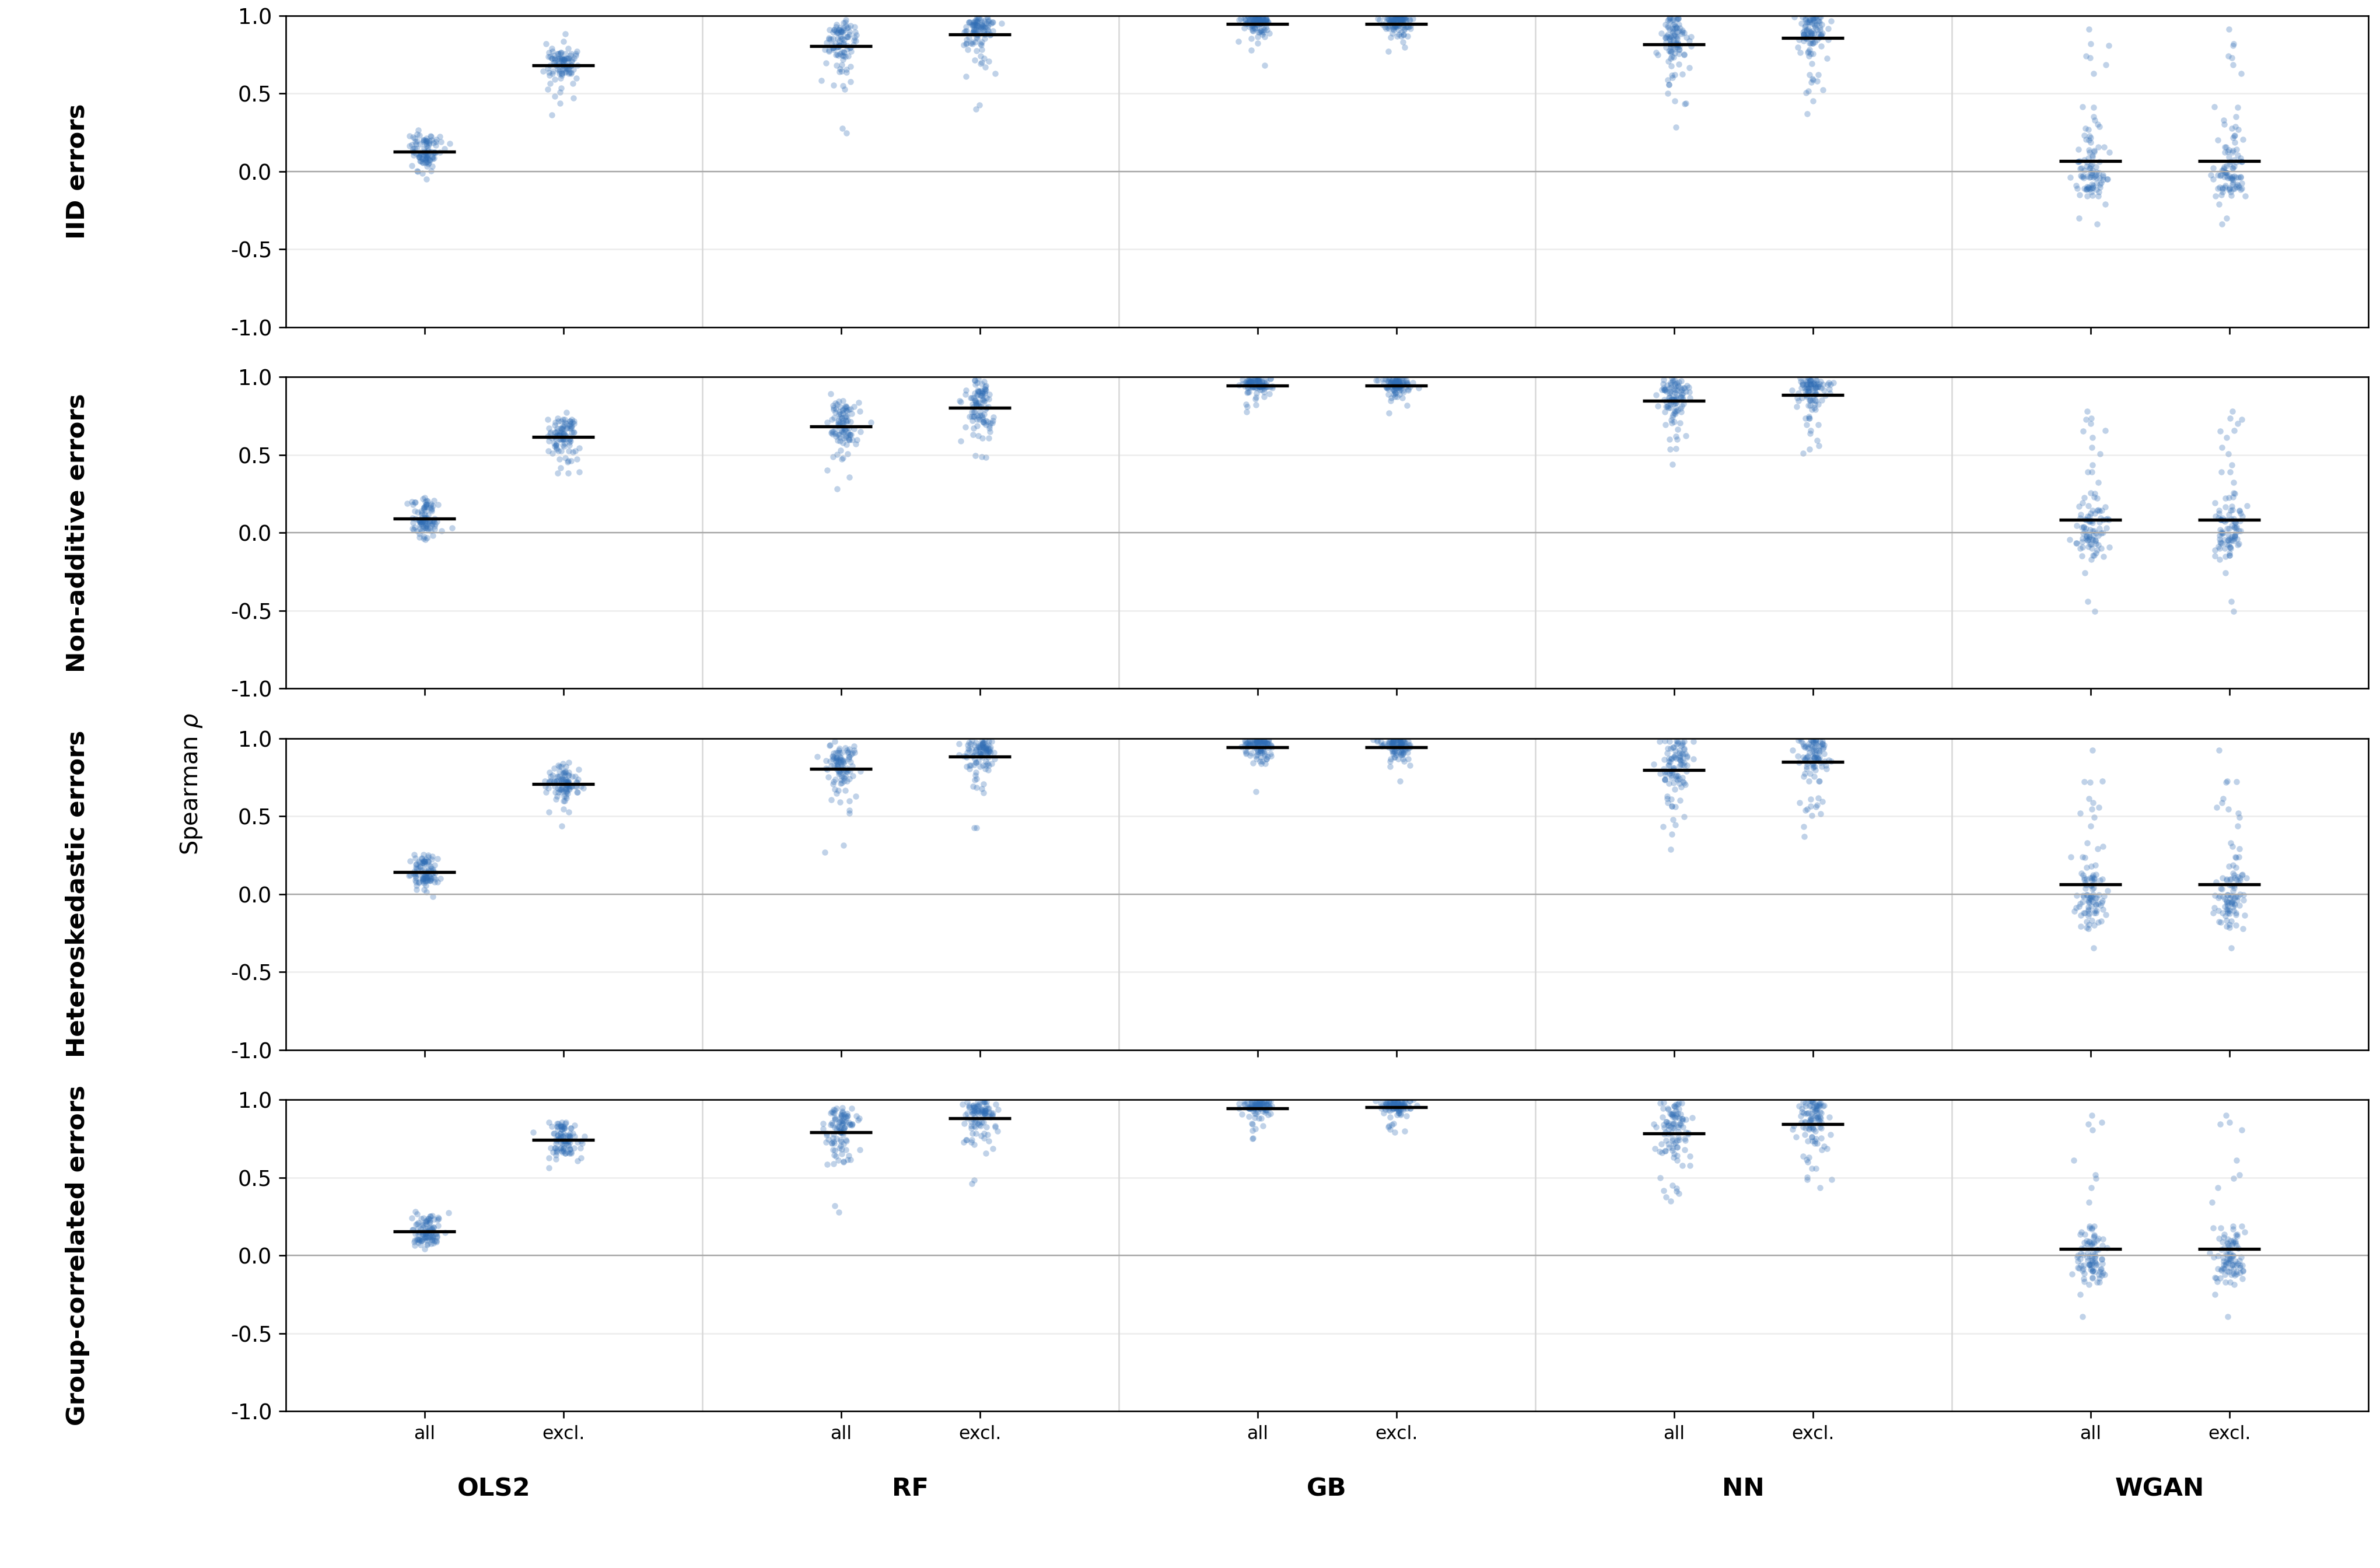
\includegraphics[width=\textwidth,height=0.445\textheight,keepaspectratio]{figures/acic_rhos_contiguous/acic_rhos_combined.png}
\par\smallskip

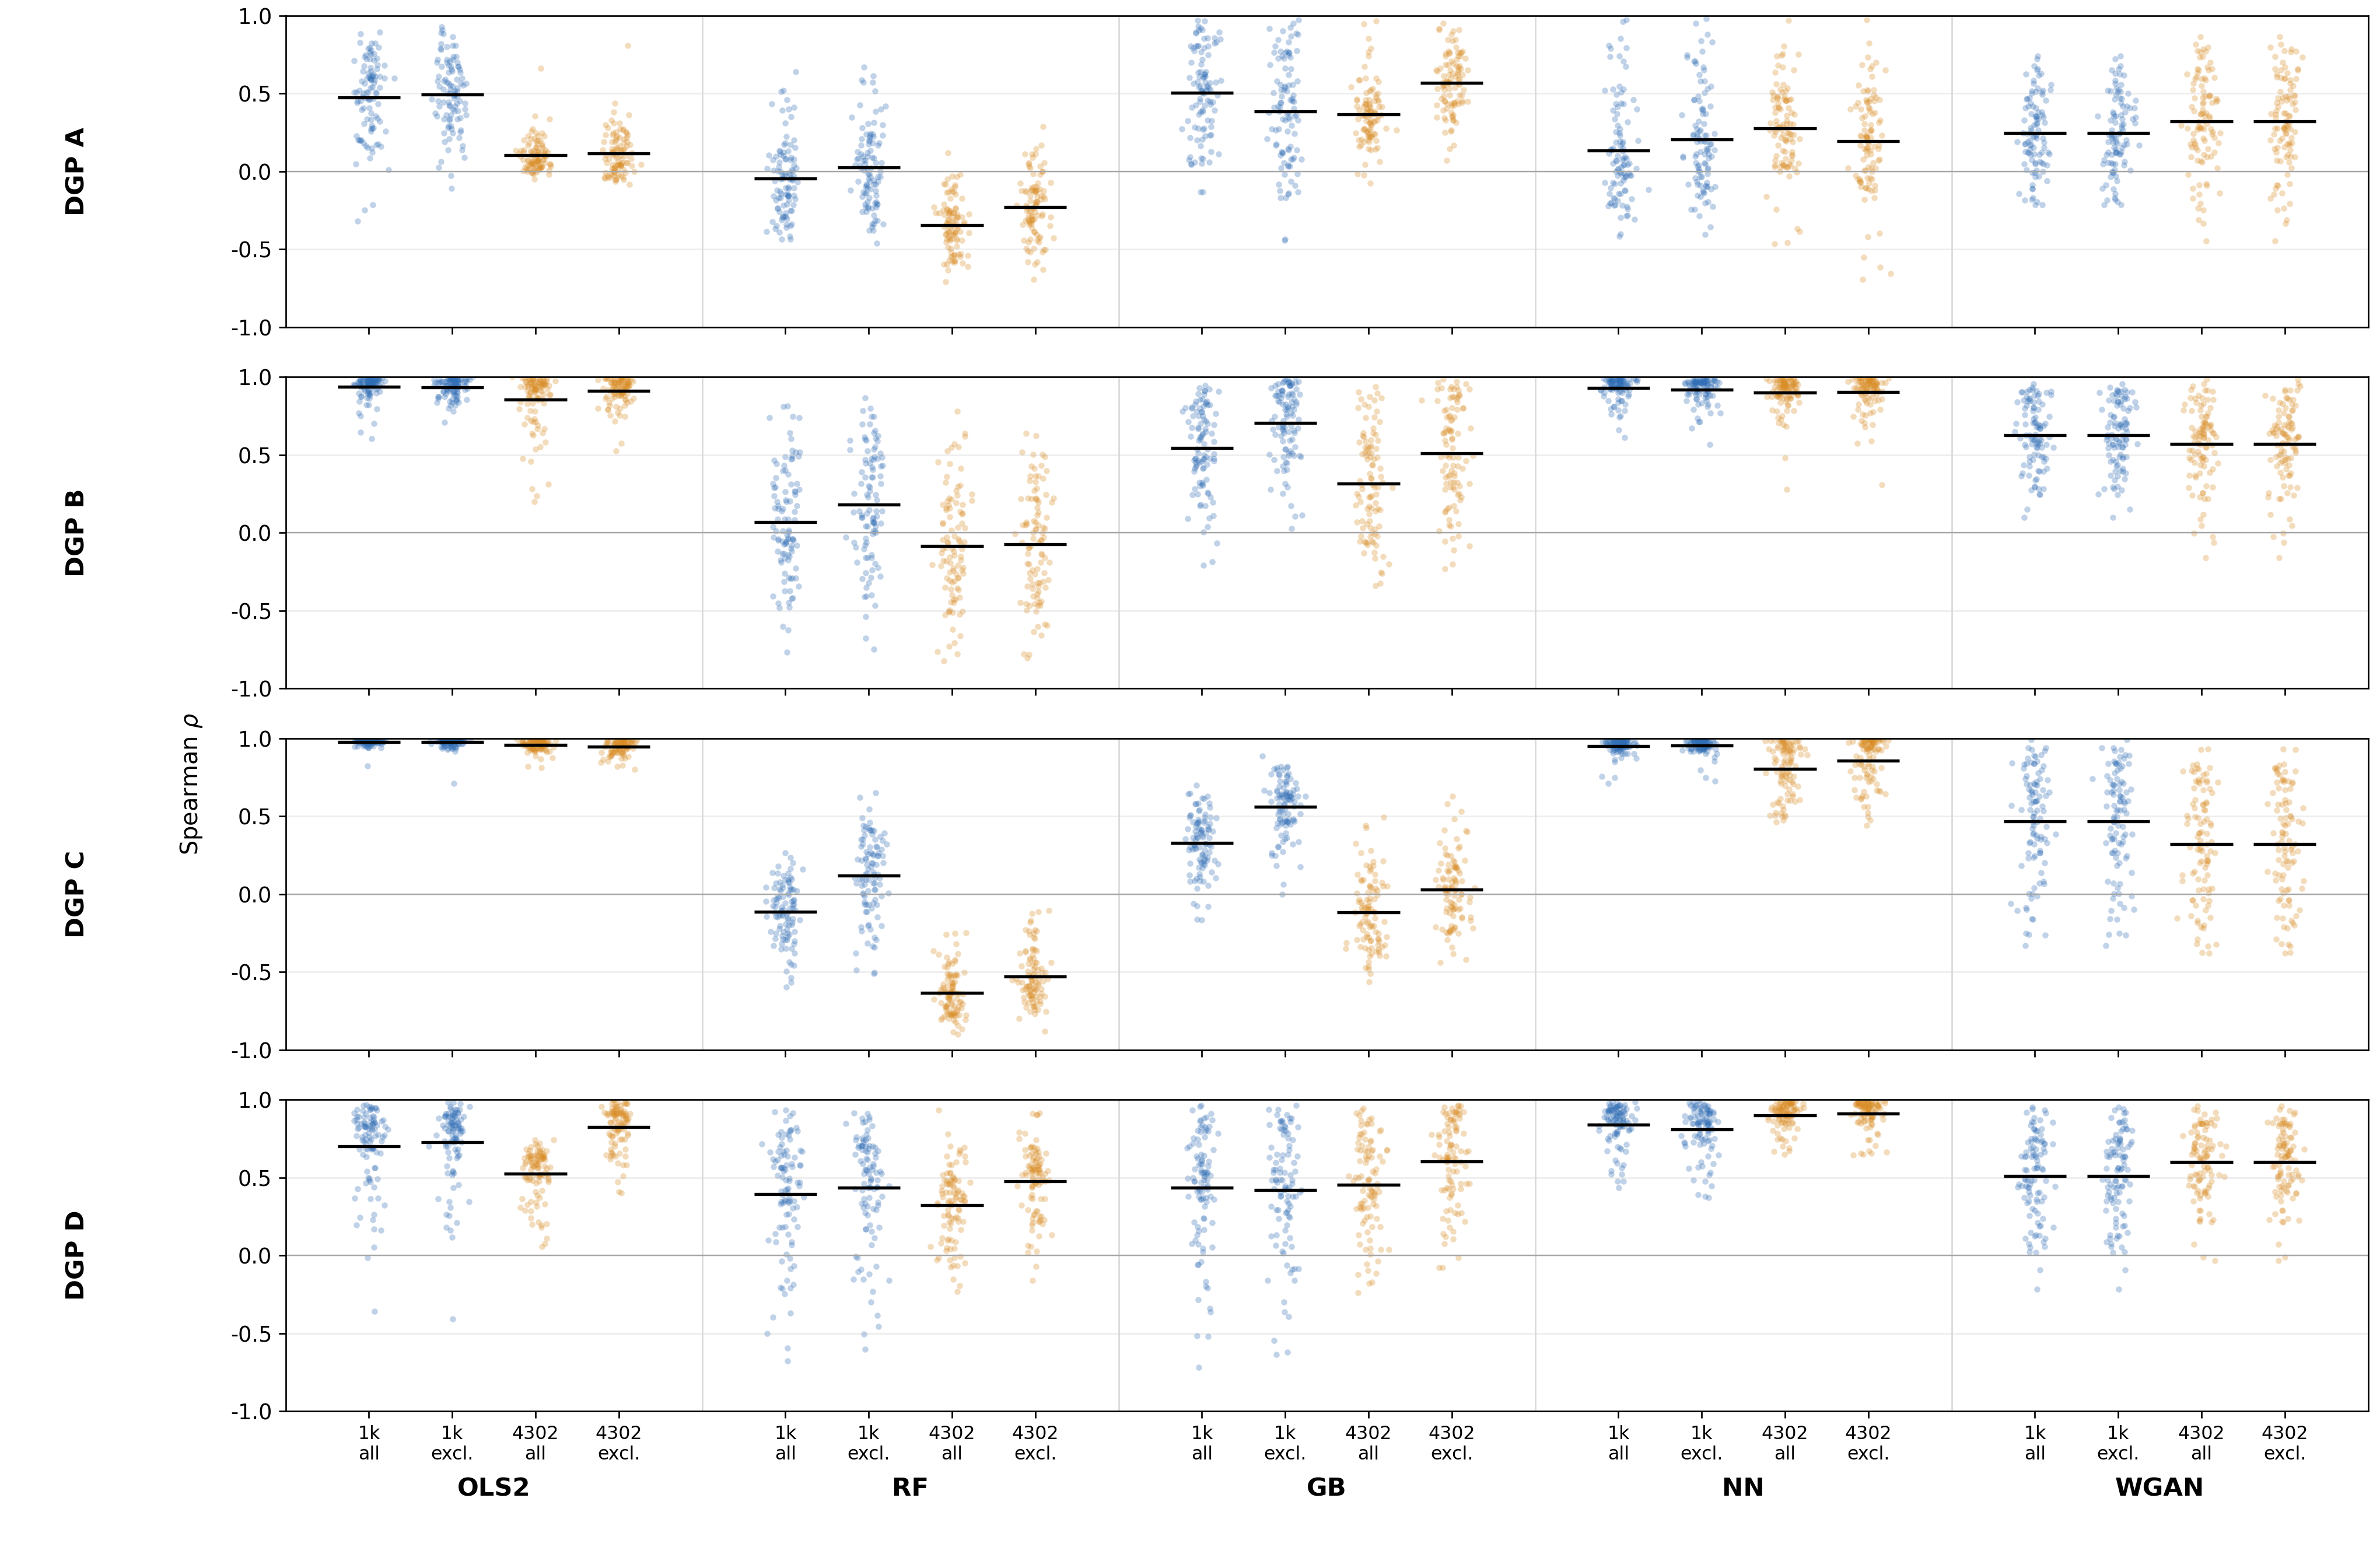
\includegraphics[width=\textwidth,height=0.445\textheight,keepaspectratio]{figures/nie_rhos_contiguous/nie_rhos_combined.png}
\caption{Per-dataset Spearman rank correlations across 100 reference datasets, using all estimators and excluding estimators sharing the simulator's outcome-model family. The upper panels show the four ACIC error structures; the lower panels show N\&W DGPs A--D, with blue and orange points denoting \(n=1000\) and \(n=4302\), respectively. Horizontal black segments indicate means.}
\label{fig:acic_rho}\label{fig:niea_rho}
\end{figure}
\FloatBarrier
\clearpage
\twocolumn
\section{Generators}
\label{app:generators}

This section describes the implementations of the original designs used to generate reference datasets before any simulator is fitted.

\subsection{ACIC 2017 designs}

The ACIC designs use the fixed \(n=4302\) covariate matrix from the Infant Health and Development Program data, available in the \href{https://github.com/vdorie/aciccomp/tree/master/2017}{ACIC 2017 repository}, with synthetic treatment and outcome mechanisms \cite{hahnAtlanticCausalInference2019}. We use the high-effect, high-noise, strong-confounding setting: \(\xi=2\), \(\eta=5/4\), and \((\kappa_1,\kappa_2)=(3,-1)\), corresponding to case 8 in their Table 2. The fitted models use eight covariates in ACIC and six in N\&W. \authorcite{hahnAtlanticCausalInference2019} distinguish the original covariate matrix from the transformed matrix used by the DGP (their Section 6.2). The formulas below use the design inputs, including indicator recodings of the cigarette-use and race variables, while retaining the original IHDP/ACIC numbering: \(X_1\) is mother's age, \(X_3\) cigarettes per day, \(X_{10}\), \(X_{14}\), and \(X_{15}\) are maternal binary health indicators, \(X_{21}\) is mother's place of birth, \(X_{24}\) is race, and \(X_{43}\) is the child's bilirubin level. Let
\[
\begin{aligned}
f(X)&=X_1+X_{43}+0.3(X_{10}-1),\\
e(X)&=\left[1+\exp\!\left\{\kappa_1f(X)+\kappa_2\right\}\right]^{-1},\\
\mu(X)&=-\sin\!\left\{F_{\!\mathcal N}^{-1}(e(X))\right\}+X_{43},\\
\tau(X)&=\xi\left\{X_3X_{24}+(X_{14}-1)-(X_{15}-1)\right\},\\
\sigma(X)&=0.4+\frac{X_{21}-1}{15},\\
\sigma_Y&=\eta\sqrt{\operatorname{Var}_n\!\left\{\mu(X)+e(X)\tau(X)\right\}},
\end{aligned}
\]
where \(F_{\!\mathcal N}^{-1}\) is the standard-normal quantile function and \(\operatorname{Var}_n\) is the variance over the fixed covariate sample. We use the quantile convention of the authors\textquotesingle{} R generator; the PDF instead prints a normal CDF in the definition of \(\mu\). For each reference dataset, treatment is redrawn independently as \(A_i\mid X_i\sim\operatorname{Bernoulli}\{e(X_i)\}\). With independent standard-normal \(\varepsilon_i\), the additive error schemes are
\[
\begin{aligned}
Y_i^{\mathrm{iid}}&=\mu(X_i)+A_i\tau(X_i)+\sigma_Y\varepsilon_i,\\
Y_i^{\mathrm{group}}&=\mu(X_i)+A_i\tau(X_i)+\sigma_Y\{0.9\varepsilon_i+0.1u_{X_{i,21}}\},\\
Y_i^{\mathrm{het}}&=\mu(X_i)+A_i\tau(X_i)+\sigma(X_i)\sigma_Y\varepsilon_i,
\end{aligned}
\]
where \(u_1,\ldots,u_{16}\) are independent standard-normal group shocks, independent of the unit-specific errors. For the non-additive design, first define
\[
\begin{aligned}
\widetilde Y_i&=\mu(X_i)+A_i\tau(X_i)+\sigma_Y\varepsilon_i,\\
a&=\frac1n\sum_{i=1}^n\{\mu(X_i)+e(X_i)\tau(X_i)\},\\
b&=1.25\sqrt{\sigma_Y^2+\operatorname{Var}_n\!\left\{\mu(X)+e(X)\tau(X)\right\}}.
\end{aligned}
\]
The observed outcome is the nonlinear transformation
\[
Y_i=13F_{\mathcal N(a,b^2)}(\widetilde Y_i)-6+\delta_i,
\qquad
\delta_i\sim\mathcal N(0,0.01^2),
\]
where \(F_{\mathcal N(a,b^2)}\) is the CDF of that normal distribution. The resulting conditional treatment effect is
\[
\begin{aligned}
\tau_{\mathrm{nonlin}}(x)
=13\Bigg[&
F_{\!\mathcal N}\!\left(
\frac{\mu(x)+\tau(x)-a}{\sqrt{\sigma_Y^2+b^2}}
\right)\\
&-F_{\!\mathcal N}\!\left(
\frac{\mu(x)-a}{\sqrt{\sigma_Y^2+b^2}}
\right)
\Bigg].
\end{aligned}
\]
\authorcite{hahnAtlanticCausalInference2019} report that the treatment-effect values accompanying the released heteroskedastic data were incorrectly calculated using the non-additive formula (their Section 6.1). Our heteroskedastic benchmark instead uses the additive outcome mechanism above and its conditional effect \(\tau(X)\), rather than those released treatment-effect values.

\subsection{N\&W designs}

For the N\&W designs \cite{nieQuasioracleEstimationHeterogeneous2021}, we use \(d=6\) covariates and generate a new \((X,A,Y)\) sample for each reference dataset. Write
\[
\begin{aligned}
Y&=b(X)+\{A-1/2\}\tau(X)+\varepsilon,\\
A\mid X&\sim\operatorname{Bernoulli}\{e(X)\},
\qquad \varepsilon\sim\mathcal N(0,1).
\end{aligned}
\]
Design A draws \(X_j\overset{\mathrm{iid}}{\sim}\operatorname{Uniform}(0,1)\); designs B--D draw \(X_j\overset{\mathrm{iid}}{\sim}\mathcal N(0,1)\). Covariates beyond \(X_5\) are noise covariates. Here \(\operatorname{trim}_{c}(u)=\min(1-c,\max(c,u))\). The functions are

\noindent\textbf{Design A}
\[
\begin{aligned}
e(X)&=\operatorname{trim}_{0.1}\!\left\{\sin(\pi X_1X_2)\right\},\\
\tau(X)&=(X_1+X_2)/2,\\
b(X)&=\sin(\pi X_1X_2)+2(X_3-0.5)^2\\
&\quad+X_4+0.5X_5.
\end{aligned}
\]
\noindent\textbf{Design B}
\[
\begin{aligned}
e(X)&=0.5,\\
\tau(X)&=X_1+\log(1+e^{X_2}),\\
b(X)&=\max\!\left\{\max(X_1+X_2,X_3),0\right\}\\
&\quad+\max(X_4+X_5,0).
\end{aligned}
\]
\noindent\textbf{Design C}
\[
\begin{aligned}
e(X)&=\{1+e^{X_2+X_3}\}^{-1},\\
\tau(X)&=1,\\
b(X)&=2\log\!\left(1+e^{X_1+X_2+X_3}\right).
\end{aligned}
\]
\noindent\textbf{Design D}
\[
\begin{aligned}
e(X)&=\{1+e^{-X_1}+e^{-X_2}\}^{-1},\\
b(X)&=\tfrac12\left[\max(X_1+X_2+X_3,0)+\max(X_4+X_5,0)\right],\\
\tau(X)&=\max(X_1+X_2+X_3,0)-\max(X_4+X_5,0).
\end{aligned}
\]

\clearpage
\section{Simulators}
\label{app:simulators}

This appendix describes the outcome models used to generate synthetic datasets within the empirical Monte Carlo design.
For generic model descriptions, we suppress the generator, reference-dataset, and Monte Carlo draw indices unless needed.

\subsection{Conditional mean--variance simulators}

Let \(\mathcal L=\{\mathrm{OLS2},\mathrm{GB},\mathrm{RF},\mathrm{NN}\}\), indexed by \(l\), be the conditional-mean outcome learners used both to construct simulators and to form causal estimators. Their conditional-mean specifications are reused for the corresponding causal estimators in Appendix~\ref{app:estimators}; the conditional-variance models below are used only to generate simulated outcomes.

The OLS2, gradient-boosting, random-forest, and neural-network simulators use a common location--scale representation that allows for heteroskedasticity,
\[
\widetilde Y_i
=
\widehat{\mu}_s(X_i,A_i)
+
\widehat{\sigma}_s(X_i,A_i)\varepsilon_i,
\]
where \(\varepsilon_i\overset{\mathrm{iid}}{\sim}\mathcal N(0,1)\). For each simulator, we obtain counterfactual conditional means
\[
\widehat{\mu}_{s,0}(X_i)
=
\widehat{\mu}_s(X_i,0),
\qquad
\widehat{\mu}_{s,1}(X_i)
=
\widehat{\mu}_s(X_i,1),
\]
and conditional standard deviations \(\widehat{\sigma}_{s,0}(X_i)\) and \(\widehat{\sigma}_{s,1}(X_i)\). A synthetic observed outcome is generated as
\[
\begin{aligned}
\widetilde Y_{i,s}^{g,m,k}
={}&
A_i^{g,m}
\left\{
\widehat{\mu}_{s,1}^{\,g,m}(X_i^{g,m})
+
\widehat{\sigma}_{s,1}^{\,g,m}(X_i^{g,m})\varepsilon_{i1}^{(k)}
\right\}\\
&+
\left(1-A_i^{g,m}\right)
\left\{
\widehat{\mu}_{s,0}^{\,g,m}(X_i^{g,m})
+
\widehat{\sigma}_{s,0}^{\,g,m}(X_i^{g,m})\varepsilon_{i0}^{(k)}
\right\}.
\end{aligned}
\]

\subsubsection{OLS2 simulator}

The OLS2 simulator fits the conditional mean as a second-order polynomial in covariates and treatment, including linear terms, squares, and all pairwise interactions. This expansion produces 54 predictor columns in ACIC and 35 in N\&W; accounting for perfect collinearities leaves 48 and 34 independent predictors, respectively, plus an intercept. The conditional variance is estimated by regressing \(\log\{(r_i^{\mathrm{OOF}})^2+\epsilon\}\) on the same terms, where \(r_i^{\mathrm{OOF}}=Y_i-\widehat\mu_{-k(i)}(X_i,A_i)\) are five-fold out-of-fold residuals and \(\epsilon=10^{-6}\widehat{\operatorname{Var}}(r^{\mathrm{OOF}})+10^{-12}\). Exponentiated predictions are rescaled so their average equals the mean squared out-of-fold residual.

\subsubsection{Gradient-boosting simulator}

The GB simulator uses \texttt{HistGradientBoostingRegressor} from Python's scikit-learn library to estimate the conditional mean of \(Y\) given \((X,A)\). Starting from \(f_0(x,a)=\overline Y\), squared-error boosting fits each regression tree \(h_b\) to the current residuals and updates the prediction:
\[
\begin{aligned}
r_{ib} &= Y_i-f_{b-1}(X_i,A_i),\\
f_b(x,a) &= f_{b-1}(x,a)+\eta h_b(x,a).
\end{aligned}
\]
Here \(\eta\) is the learning rate, and after \(B\) trees the fitted mean is \(\widehat\mu_{\mathrm{GB}}=f_B\). Both GB models use \(\eta=0.05\), at most 500 trees, and a maximum tree depth of 6, without hyperparameter tuning. Tree splits capture nonlinear effects and interactions, including interactions with treatment. Histogram binning speeds up the search for splits.

For the variance, let \(r_i^{\mathrm{OOF}}=Y_i-\widehat\mu_{-k(i)}(X_i,A_i)\) denote five-fold out-of-fold residuals, where \(-k(i)\) excludes the fold containing unit \(i\). A second GB model \(\widehat g\) predicts the log-squared residual target:
\[
\begin{aligned}
v_i &= \log\!\left[(r_i^{\mathrm{OOF}})^2+\epsilon\right],\\
\widehat\sigma_{\mathrm{GB}}^2(x,a) &= c\exp\!\left\{\widehat g(x,a)\right\}.
\end{aligned}
\]
We set \(\epsilon=10^{-6}\widehat{\operatorname{Var}}(r^{\mathrm{OOF}})+10^{-12}\), using the empirical residual variance with divisor \(n\), to keep the logarithm finite. The multiplier \(c\) makes the average predicted variance equal to the average squared out-of-fold residual.

\subsubsection{Random-forest simulator}

The RF simulator uses \texttt{RandomForestRegressor} from Python's scikit-learn library to estimate the conditional mean of \(Y\) given \((X,A)\). Each regression tree \(h_t\) is fitted to a bootstrap sample, choosing splits to reduce squared error. The forest averages the predictions of \(T\) trees:
\[
\widehat\mu_{\mathrm{RF}}(x,a)
=\frac{1}{T}\sum_{t=1}^{T}h_t(x,a).
\]
Here \(h_t(x,a)\) is the mean outcome in the leaf containing \((x,a)\). Both RF models use \(T=800\) trees, all predictors at each split, a minimum leaf size of one, and no maximum depth, without hyperparameter tuning. Tree splits capture nonlinear effects and interactions, while averaging reduces the variability of individual trees.

For the variance, let \(r_i^{\mathrm{OOB}}=Y_i-\widehat\mu_{\mathrm{OOB}}(X_i,A_i)\) denote out-of-bag residuals, where \(\widehat\mu_{\mathrm{OOB}}\) averages only trees whose bootstrap samples exclude unit \(i\). A second RF model \(\widehat g\) predicts the log-squared residual target:
\[
\begin{aligned}
v_i &= \log\!\left[(r_i^{\mathrm{OOB}})^2+\epsilon\right],\\
\widehat\sigma_{\mathrm{RF}}^2(x,a) &= c\exp\!\left\{\widehat g(x,a)\right\}.
\end{aligned}
\]
We set \(\epsilon=10^{-6}\widehat{\operatorname{Var}}(r^{\mathrm{OOB}})+10^{-12}\), using the empirical residual variance with divisor \(n\), to keep the logarithm finite. The multiplier \(c\) makes the average predicted variance equal to the average squared out-of-bag residual.

\subsubsection{Neural-network simulator}

The NN simulator uses \texttt{MLPRegressor} from Python's scikit-learn library to estimate the conditional mean of \(Y\) given \((X,A)\). After standardizing the predictors with \texttt{StandardScaler}, the network applies two hidden layers and a linear output:
\[
\begin{aligned}
h_\ell &= \operatorname{ReLU}(W_\ell h_{\ell-1}+b_\ell),\qquad \ell=1,2,\\
\widehat\mu_{\mathrm{NN}}(x,a) &= w_3^{\mathsf T}h_2+b_3.
\end{aligned}
\]
Here \(h_0\) is the standardized vector \((x,a)\), \(\operatorname{ReLU}(u)=\max(0,u)\) acts elementwise, and the weights and biases are fitted by minimizing squared-error loss with an L2 penalty. Both NN models use hidden layers of 64 and 32 units, Adam with initial learning rate \(10^{-3}\), penalty parameter \(\alpha=10^{-4}\), batch size 256, and at most 400 epochs, without hyperparameter tuning. Early stopping uses a 10\% validation split, patience of 25 epochs, and tolerance \(10^{-3}\) in validation \(R^2\). The nonlinear layers capture covariate effects and interactions.

For the variance, let \(r_i^{\mathrm{OOF}}=Y_i-\widehat\mu_{-k(i)}(X_i,A_i)\) denote five-fold out-of-fold residuals, where \(-k(i)\) excludes the fold containing unit \(i\). A second NN model \(\widehat g\) predicts the log-squared residual target:
\[
\begin{aligned}
v_i &= \log\!\left[(r_i^{\mathrm{OOF}})^2+\epsilon\right],\\
\widehat\sigma_{\mathrm{NN}}^2(x,a) &= c\exp\!\left\{\widehat g(x,a)\right\}.
\end{aligned}
\]
We set \(\epsilon=10^{-6}\widehat{\operatorname{Var}}(r^{\mathrm{OOF}})+10^{-12}\), using the empirical residual variance with divisor \(n\), to keep the logarithm finite. The multiplier \(c\) makes the average predicted variance equal to the average squared out-of-fold residual.

\subsection{Conditional generative simulator}

\noindent\textbf{Conditional Wasserstein generative adversarial network.}

We use the WGAN with gradient penalty developed by \authorcite{gulrajaniImprovedTrainingWasserstein2017}, following \authorcite{atheyUsingWassersteinGenerative2024} in fitting separate conditional models for the two treatment arms. Separate generators and critics are fitted in the control and treated groups. For treatment arm \(a\), the generator represents the conditional outcome distribution as
\[
\widetilde Y
=
G_{\theta,a}(Z,X),
\qquad
Z\sim\mathcal N(0,I).
\]
Each generator takes standardized covariates and a 10-dimensional standard-normal noise vector as inputs and has three hidden layers of 128 units with layer normalization and leaky-ReLU activations. The critic has three hidden layers of 128 units with leaky-ReLU activations and maps an outcome--covariate pair to a scalar score.

For each minibatch, the critic is updated five times to assign higher scores to observed outcomes than to generated outcomes, while the generator is updated to increase its generated outcomes' critic scores. We enforce the critic's Lipschitz constraint with the WGAN gradient penalty. Writing \(Y^G=G_{\theta,a}(Z,X)\), the losses are
\[
\begin{aligned}
\mathcal L_D
&=
\mathbb E\!\left[D_{\omega,a}(Y^G,X)\right]
-\mathbb E\!\left[D_{\omega,a}(Y,X)\right]\\
&\quad+\lambda\,
\mathbb E\!\left[\left(\left\lVert\nabla_{\bar Y}D_{\omega,a}(\bar Y,X)\right\rVert_2-1\right)^2\right],\\
\mathcal L_G
&=-\mathbb E\!\left[D_{\omega,a}(Y^G,X)\right],
\end{aligned}
\]
where \(\bar Y\) interpolates between observed and generated outcomes and \(\lambda=10\). We train each arm for 5000 epochs with batch size 512, using Adam with \((\beta_1,\beta_2)=(0,0.9)\) and learning rates \(5\times10^{-5}\) for the generator and \(2\times10^{-4}\) for the critic.

Adversarial losses do not provide a conventional convergence criterion. We therefore retain the checkpoint with the smallest average exact one-dimensional Wasserstein-1 distance between observed and generated standardized outcomes, averaged over five draws for each treatment arm. The distance is computed at the first epoch, every 200 epochs, and the final epoch.

After training, synthetic outcomes are generated by drawing new values of \(Z\) while keeping \(X_i^{g,m}\) and \(A_i^{g,m}\) fixed,
\[
\widetilde Y_{i,s}^{g,m,k}
=
G_{\widehat{\theta},A_i^{g,m}}
\left(
Z_i^{(k)},X_i^{g,m}
\right).
\]
Although the WGAN learns the full conditional distribution, its counterfactual means are needed to compute the estimand. We approximate them with \(B=10{,}000\) Monte Carlo draws per treatment and reference covariate vector,
\[
\widehat{\mu}_{s,a}^{\,g,m}(X_i^{g,m})
\approx
\frac{1}{B}
\sum_{b=1}^{B}
G_{\widehat{\theta},a}
\left(
Z_i^{(b)},X_i^{g,m}
\right).
\]

\clearpage
\section{Estimators}
\label{app:estimators}

This appendix complements the simulator description by detailing the causal estimators used in the benchmark comparison. Here \((X_i,A_i,Y_i)\) denotes unit \(i\) in the dataset to which the estimator is applied; generator, reference-dataset, simulator, and draw indices are suppressed. The outcome models that are used by some of the estimators intentionally follow the same conditional-mean specifications as the learners used to construct the simulators, \(\mathcal L=\{\mathrm{OLS2},\mathrm{GB},\mathrm{RF},\mathrm{NN}\}\). See Appendix~\ref{app:simulators} for more details.

\subsection{G-computation estimators}

For each outcome learner \(l\) in \(\mathcal L\), we estimate
\[
\widehat{\mu}_{l,a}(x)
\approx
\mathbb E[Y\mid A=a,X=x].
\]
Throughout the formulas below, \(\widehat\mu_{l,a}(X_i)\) denotes an out-of-fold prediction from a model fitted without the fold containing unit \(i\); fold indices are suppressed.
The G-computation estimator is
\[
\widehat{\Phi}_{l,\mathrm{Gcomp}}
=
\frac{1}{n}
\sum_{i=1}^{n}
\left\{
\widehat{\mu}_{l,1}(X_i)
-
\widehat{\mu}_{l,0}(X_i)
\right\}.
\]

OLS1 is a pooled additive linear regression of the outcome on treatment and covariates; its reported estimate is the treatment coefficient.

\subsection{Inverse probability weighting}
\label{app:ipw}

We estimate the propensity score, \mbox{\(e(x)=\Pr(A=1\mid X=x)\)}, using a five-fold cross-fitted \texttt{GradientBoostingClassifier} from scikit-learn, following \authorcite{chernozhukovDoubleDebiasedMachine2018}. We denote the fitted score by \(\widehat e(x)\). The classifier sequentially combines shallow trees to predict treatment status by minimizing logistic loss. We use the normalized IPW estimator \cite{luncefordStratificationWeightingPropensity2004},
\[
\widehat{\Phi}_{\mathrm{IPW}}
=
\frac{
\sum_{i=1}^{n}
A_iY_i/\widehat e(X_i)
}{
\sum_{i=1}^{n}
A_i/\widehat e(X_i)
}
-
\frac{
\sum_{i=1}^{n}
(1-A_i)Y_i/\{1-\widehat e(X_i)\}
}{
\sum_{i=1}^{n}
(1-A_i)/\{1-\widehat e(X_i)\}
}.
\]
Estimated propensity scores are truncated to \([0.01,0.99]\), corresponding to a trimming threshold of \(\delta=0.01\).

\subsection{Augmented inverse probability weighting}

For each of the outcome learners \(l\) in \(\mathcal L\), and using the same estimated propensity scores as for the IPW estimator, the AIPW estimator \cite{bangDoublyRobustEstimation2005} is
\[
\begin{aligned}
\widehat{\Phi}_{l,\mathrm{AIPW}}
={}&
\frac{1}{n}
\sum_{i=1}^{n}
\left[
\widehat{\mu}_{l,1}(X_i)
-
\widehat{\mu}_{l,0}(X_i)
\right.\\
&\left.
+
\frac{
A_i\{Y_i-\widehat{\mu}_{l,1}(X_i)\}
}{
\widehat e(X_i)
}
-
\frac{
(1-A_i)\{Y_i-\widehat{\mu}_{l,0}(X_i)\}
}{
1-\widehat e(X_i)
}
\right].
\end{aligned}
\]

\subsection{Targeted maximum likelihood estimation}

TMLE \cite{vanderlaanTargetedMaximumLikelihood2006} starts from initial estimates \(\widehat{\mu}_{l,0}(X_i)\) and \(\widehat{\mu}_{l,1}(X_i)\), for each \(l\) in \(\mathcal L\), and updates them using the estimated propensity score from the IPW estimator. For the continuous outcome considered here, define the clever covariate
\[
H_{\widehat e}(A_i,X_i)
=
\frac{A_i}{\widehat e(X_i)}
-
\frac{1-A_i}{1-\widehat e(X_i)}.
\]

The fluctuation parameter is estimated as
\[
\widehat{\varepsilon}
=
\frac{
\sum_{i=1}^{n}
H_{\widehat e}(A_i,X_i)
\left\{
Y_i-\widehat{\mu}_{l,A_i}(X_i)
\right\}
}{
\sum_{i=1}^{n}
H_{\widehat e}(A_i,X_i)^2
}.
\]
The targeted predictions are
\[
\begin{aligned}
\widehat{\mu}^{\star}_{l,1}(X_i)
&=\widehat{\mu}_{l,1}(X_i)+\frac{\widehat{\varepsilon}}{\widehat e(X_i)},\\
\widehat{\mu}^{\star}_{l,0}(X_i)
&=\widehat{\mu}_{l,0}(X_i)-\frac{\widehat{\varepsilon}}{1-\widehat e(X_i)}.
\end{aligned}
\]
The TMLE estimator is then
\[
\widehat{\Phi}_{l,\mathrm{TMLE}}
=
\frac{1}{n}
\sum_{i=1}^{n}
\left\{
\widehat{\mu}^{\star}_{l,1}(X_i)
-
\widehat{\mu}^{\star}_{l,0}(X_i)
\right\}.
\]

\subsection{Bayesian causal forest}

Bayesian causal forest (BCF) \cite{hahnBayesianRegressionTree2020} separates the outcome surface into a baseline component and a treatment-effect component:
\[
\mathbb E[Y\mid X=x,A=a]
=
\mu\{x,\widehat e(x)\}
+
a\,\tau(x).
\]
The fitted propensity score \(\widehat e(x)\) enters the baseline component. For BCF, we fit the gradient-boosting propensity model in sample, trim its predictions to the interval \([0.01,0.99]\), and standardize the outcome before fitting.

The \texttt{stochtree} algorithm represents \(\mu\) and \(\tau\) as separate sums of trees. It first performs 10 grow-from-root iterations, which construct an initial pair of tree ensembles from the data. It then runs an MCMC backfitting procedure. Conditional on the current treatment-effect forest, the baseline forest is updated using the remaining outcome residuals; conditional on the current baseline forest, the treatment-effect forest is updated using the remaining treatment-associated residuals. Thus, the trees in the two ensembles are repeatedly modified while accounting for the other component. After 20 burn-in iterations, we retain 30 posterior draws; posterior-mean potential-outcome predictions average over those draws.

We use 250 trees for the baseline forest and 50 for the treatment-effect forest. The treatment-effect forest has a shallower-tree prior (\(\alpha=0.25,\beta=3\)) than the baseline forest (\(\alpha=0.95,\beta=2\)), which shrinks effect heterogeneity more strongly than baseline outcome variation. We use the homoskedastic version of the model.

For each covariate vector, we obtain posterior-mean predictions under both treatment values, \(\widehat m(x,1)\) and \(\widehat m(x,0)\), and form
\[
\widehat\tau(x)=\widehat m(x,1)-\widehat m(x,0).
\]
The BCF G-computation estimator averages these predicted effects over the observed covariates:
\[
\widehat{\Phi}_{\mathrm{BCF}}
=
\frac{1}{n}
\sum_{i=1}^{n}
\widehat\tau(X_i).
\]

\clearpage
\section{Outcome-distribution distances}
\label{app:distances}

For each original reference dataset, let \(Y_i^0\) denote the observed outcome for unit \(i\) and \(\widetilde Y_i^{(k)}\) the outcome for that unit in the \(k\)-th dataset generated by simulator \(s\). We calculate each metric from the full samples \(\{Y_i^0\}_{i=1}^n\) and \(\{\widetilde Y_i^{(k)}\}_{i=1}^n\), then average it over the \(K\) Monte Carlo outcome draws:
\[
d_\ell^{g,m,s}=\frac{1}{K}\sum_{k=1}^{K}D_\ell\!\left(\{Y_i^0\}_{i=1}^n,\{\widetilde Y_i^{(k)}\}_{i=1}^n\right).
\]
We report three distributional distances. Writing \(F\) and \(\widetilde F\) for the two empirical CDFs, and \(Y^0_{(j)}\) and \(\widetilde Y_{(j)}\) for their ordered values, we define the distances as
\[
\begin{aligned}
W_1&=\frac{1}{n}\sum_{j=1}^{n}\left|Y^0_{(j)}-\widetilde Y_{(j)}\right|,\\
\mathrm{KS}&=\sup_y\left|F(y)-\widetilde F(y)\right|,\\
\mathrm{Energy}&=\left\{2\int_{-\infty}^{\infty}\left[F(y)-\widetilde F(y)\right]^2\,dy\right\}^{1/2}.
\end{aligned}
\]
These distances compare the full marginal outcome distributions.

Finally, within each reference dataset \(m\) and setting \(g\), we compute the Pearson correlation across the five simulators between \(d_\ell^{g,m,s}\) and their Spearman ranking fidelity \(\rho^{g,m,s}\). We report the mean of these correlations over the 100 reference datasets in each setting. Thus, simulators are compared on the same reference dataset rather than pooled across reference datasets. The alignment-excluded columns use \(\rho_{\mathrm{excl}}^{g,m,s}\), excluding estimators aligned with each simulator.

\end{document}
